\documentclass[]{mwart}

\usepackage{polski}
\usepackage[utf8]{inputenc}

\usepackage{amsthm}
\usepackage{amsmath}
\usepackage{amssymb}

\usepackage{mdframed}
\usepackage{hyperref}
\usepackage[draft%      % dla obrazkow zakomentowac draft
]{graphicx}  
\usepackage{url}
\usepackage{enumitem}
\usepackage{verbatim}



\usepackage{caption}    
\usepackage{float}      



\usepackage{fancyhdr}
\pagestyle{fancy}
\fancyhf{}

\fancyhead[L]{
\includegraphics[height=0.666cm]{wspolne_dla_wszystkich/logo_projektu.png}}
\fancyhead[C]{\textit{Poprawa jakości zdjęć}}
\fancyhead[R]{
\includegraphics[height=0.9cm]{wspolne_dla_wszystkich/logo_uczelni.png}}
\fancyfoot[C]{\thepage}

\setlength{\headheight}{20pt}  



\usepackage{listings}
\usepackage{xcolor} 

% \makeatletter
% \@addtoreset{section}{part}
% \makeatother

\begin{document}








\thispagestyle{empty}

\begin{figure}[h]
    \centering
    
\includegraphics[width=1\textwidth]{wspolne_dla_wszystkich/logo_uczelni.png}
\end{figure}


\begin{center}
    {\LARGE \textbf{Poprawa jakości skanów zdjęć wykonanych techniką analogową
        }} \\[0.3cm]
    {\large \textbf{Raport II}} \\[0.2cm]
    \textit{projekt realizowany pod opieką prof. dr hab. inż. Artura Przelaskowskiego}

\end{center}

\begin{figure}[h]
    \centering
    
\includegraphics[width=1\textwidth]{wspolne_dla_wszystkich/logo_projektu.png}
\end{figure}

\vfill
\begin{abstract}
    Zbiór raportów projektu poprawy jakości cyfrowych skanów zdjęć wykonanych techniką
    analogową przez grupę nr 9 (wtorkową z godziny 18)
    w składzie:  Bartosz Wójcik, Katarzyna Szwed, Natalia Szymańska,
    Patrycja Szałajko, Aleksandra Wójcik, Karol Sęk, Michał Juszkiewicz, Filip Sajko.
\end{abstract}


\newpage
\tableofcontents
\newpage





























































\part{}
\thispagestyle{empty}

\begin{figure}[h]
    \centering
    
\includegraphics[width=1\textwidth]{wspolne_dla_wszystkich/logo_uczelni.png}
\end{figure}

%    \title{Projekt poprawy jakości zdjęć \\ \large{Raport 1}}
%    \date{\today}
%    %\author{\textit{Pod opieką: prof. dr hab. inż. Artura Przylaskowskiego}}
%    \maketitle
%    \begin{center}
%        \textit{Pod opieką: prof. dr hab. inż. Artura Przylaskowskiego}
%    \end{center}

\begin{center}
    {\LARGE \textbf{Projekt poprawy jakości zdjęć analogowych i cyfrowych o skrajnej jasności}} \\[0.3cm]
    {\large \textbf{Raport I}} \\[0.2cm]
    \textit{projekt realizowany pod opieką prof. dr hab. inż. Artura Przelaskowskiego}

\end{center}

\begin{figure}[h]
    \centering
    
\includegraphics[width=1\textwidth]{wspolne_dla_wszystkich/logo_projektu.png}
\end{figure}

\vfill
\begin{abstract}
    Raport 1 projektu poprawy jakości zdjęć wykonanych analogowych przez grupę wtorkową z godziny 18
    w składzie:  Bartosz Wójcik, Katarzyna Szwed, Natalia Szymańska,
    Patrycja Szałajko, Aleksandra Wójcik, Karol Sęk, Michał Juszkiewicz, Filip Sajko.

    W tym raporcie skupimy się na opisie procesu wyboru tematu projektu, jego definiowaniu
    i planach jego analizy i rozwiązania. Ponadto wykonamy zdjęcia i zaczniemy je analizować.
\end{abstract}



\newpage



\section{Wstęp}
\subsection{Wybór problemu}
Podczas wyboru tematu projektu kierowaliśmy się użytecznością
i ponadczasowością naszej pracy oraz tym, żeby nasz program
rozwiązywał problem,  który zauważamy na co dzień. Zebraliśmy
kilka naszych najlepszych pomysłów.

Były to: silnik szachowy, inteligentne
rekomendacje muzyki, wydobywanie detali ze zdjęć o ekstremalnej
jasności, opracowywanie wykresów związków chemicznych.
Dodatkowo przeprowadziliśmy ankietę wśród wybranych 27
studentów naszej uczelni. Zapytaliśmy ich, rozwiązanie
którego z powyższych problemów chcieliby zobaczyć.

Wyniki ankiety przedstawiamy poniżej:


\begin{figure}[H]
    \centering
    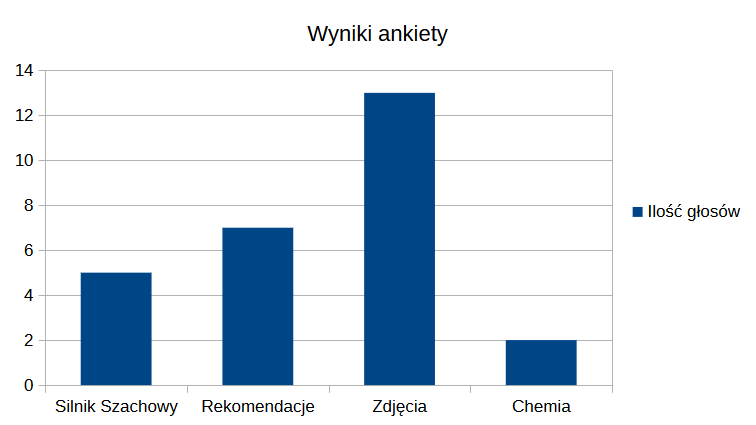
\includegraphics[width=1\textwidth]{Photos1/wyniki_ankiety.png}
\end{figure}




Jak widać zdecydowanie największą popularnością
cieszył się pomysł stworzenia programu poprawiającego jakość zdjęć.

\subsection{Cel projektu}
W ramach tego projektu skoncentrujemy się na opracowaniu metod
umożliwiających stworzenie algorytmu, który normalizuje jasność
zdjęć charakteryzujących się niedoświetleniem lub
prześwietleniem. Na podstawie tego algorytmu planujemy opracować
przyjazną użytkownikowi aplikację, dedykowaną poprawie jakości
amatorskich fotografii. Odbiorcami naszego projektu są zarówno
miłośnicy fotografii analogowej, jak i entuzjaści, którzy nie
dysponują zaawansowanym sprzętem fotograficznym, a także
wszyscy ci, którzy chcą wydobyć z archiwów rodzinnych
nową jakość.

Fotografia analogowa, w przeciwieństwie do fotografii cyfrowej,
nie pozwala na weryfikację efektów pracy tuż po wykonaniu zdjęcia.
O błędach technicznych fotograf dowiaduje się dopiero po wywołaniu
kliszy, co nie pozwala na wprowadzanie poprawek na bieżąco.
Kluczowym aspektem wykonania poprawnej fotografii jest odpowiednie
naświetlenie zdjęcia -- aby uniknąć utraty detali w światłach i cieniach.

Naszym celem jest poprawianie jakości i wyciąganie szczegółów
z zdjęć, w których te szczegóły zostały ukryte i utracone w wyniku
niedoświetlenia i prześwietlenia.

\subsection{Wykorzystywane materiały}
Badania będziemy przeprowadzać z wykorzystaniem zdjęć zrobionych
zarówno przy użyciu aparatu analogowego, jak i cyfrowego. Problemy,
które dotykają fotografii analogowej łatwo powtórzyć na aparacie cyfrowym
ustawiając korektę ekspozycji.
Celowo zrobimy zdjęcia jednego ujęcia o różnym poziomie naświetlenia tak,
abyśmy mogli na nich testować algorytm wiedząc, jakich wyników powinniśmy
się spodziewać. Dodatkowo zależy nam na pozyskaniu informacji w jaki sposób zdjęcia doświetlone niepoprawnie odstają od poprawnej ekspozycji.
Zależy nam, aby zdjęcia były o różnorodnej tematyce -- od zdjęć
natury przez portrety po zdjęcia architektury tak, aby mieć pewność, że nasza
metoda ma szerokie zastosowanie w życiu codziennym.


\subsection{Dobór zdjęć}
Będziemy pracować na wysokiej jakości cyfrowych skanach filmu zdjęć
analogowych, a także na typowych dla nas cyfrowych zdjęciach.
Posłużymy się archiwalnymi zdjęciami znalezionymi w
rodzinnych albumach, naszych własnych kolekcjach i wykonanymi
celowo na potrzeby tego projektu.

W tym celu kilkoro członków naszego zespołu chwyciło
za aparaty, i ruszyło fotografować świat!

\newpage
\section{Zdjęcia!}
Kilka przykładowych zdjęć spośród zebranych przez nas, które obrazują problem
utraty szczegółów zdjęć analogowych w przypadku ich niedoświetlenia. \newline

Dalej znajdują się także porównania kilku wybranych zdjęć wykonanych
aparatem cyfrowym przy różnych ustawieniach ekspozycji. Dla zdjęć
cyfrowych najwięcej detali traconych jest w prześwietlonych punktach.











\begin{figure}[H]
    \centering
    \includegraphics[angle=90, width=\linewidth, keepaspectratio]{Photos1/photos/analog6.jpg}
    \caption{Zdjęcie niedoświetlone}
\end{figure}
\begin{figure}[H]
    \centering
    \includegraphics[angle=90, width=\linewidth, keepaspectratio]{Photos1/photos/analog7.jpg}
    \caption{Zdjęcie doświetlone}
\end{figure}



\begin{figure}[H]
    \centering
    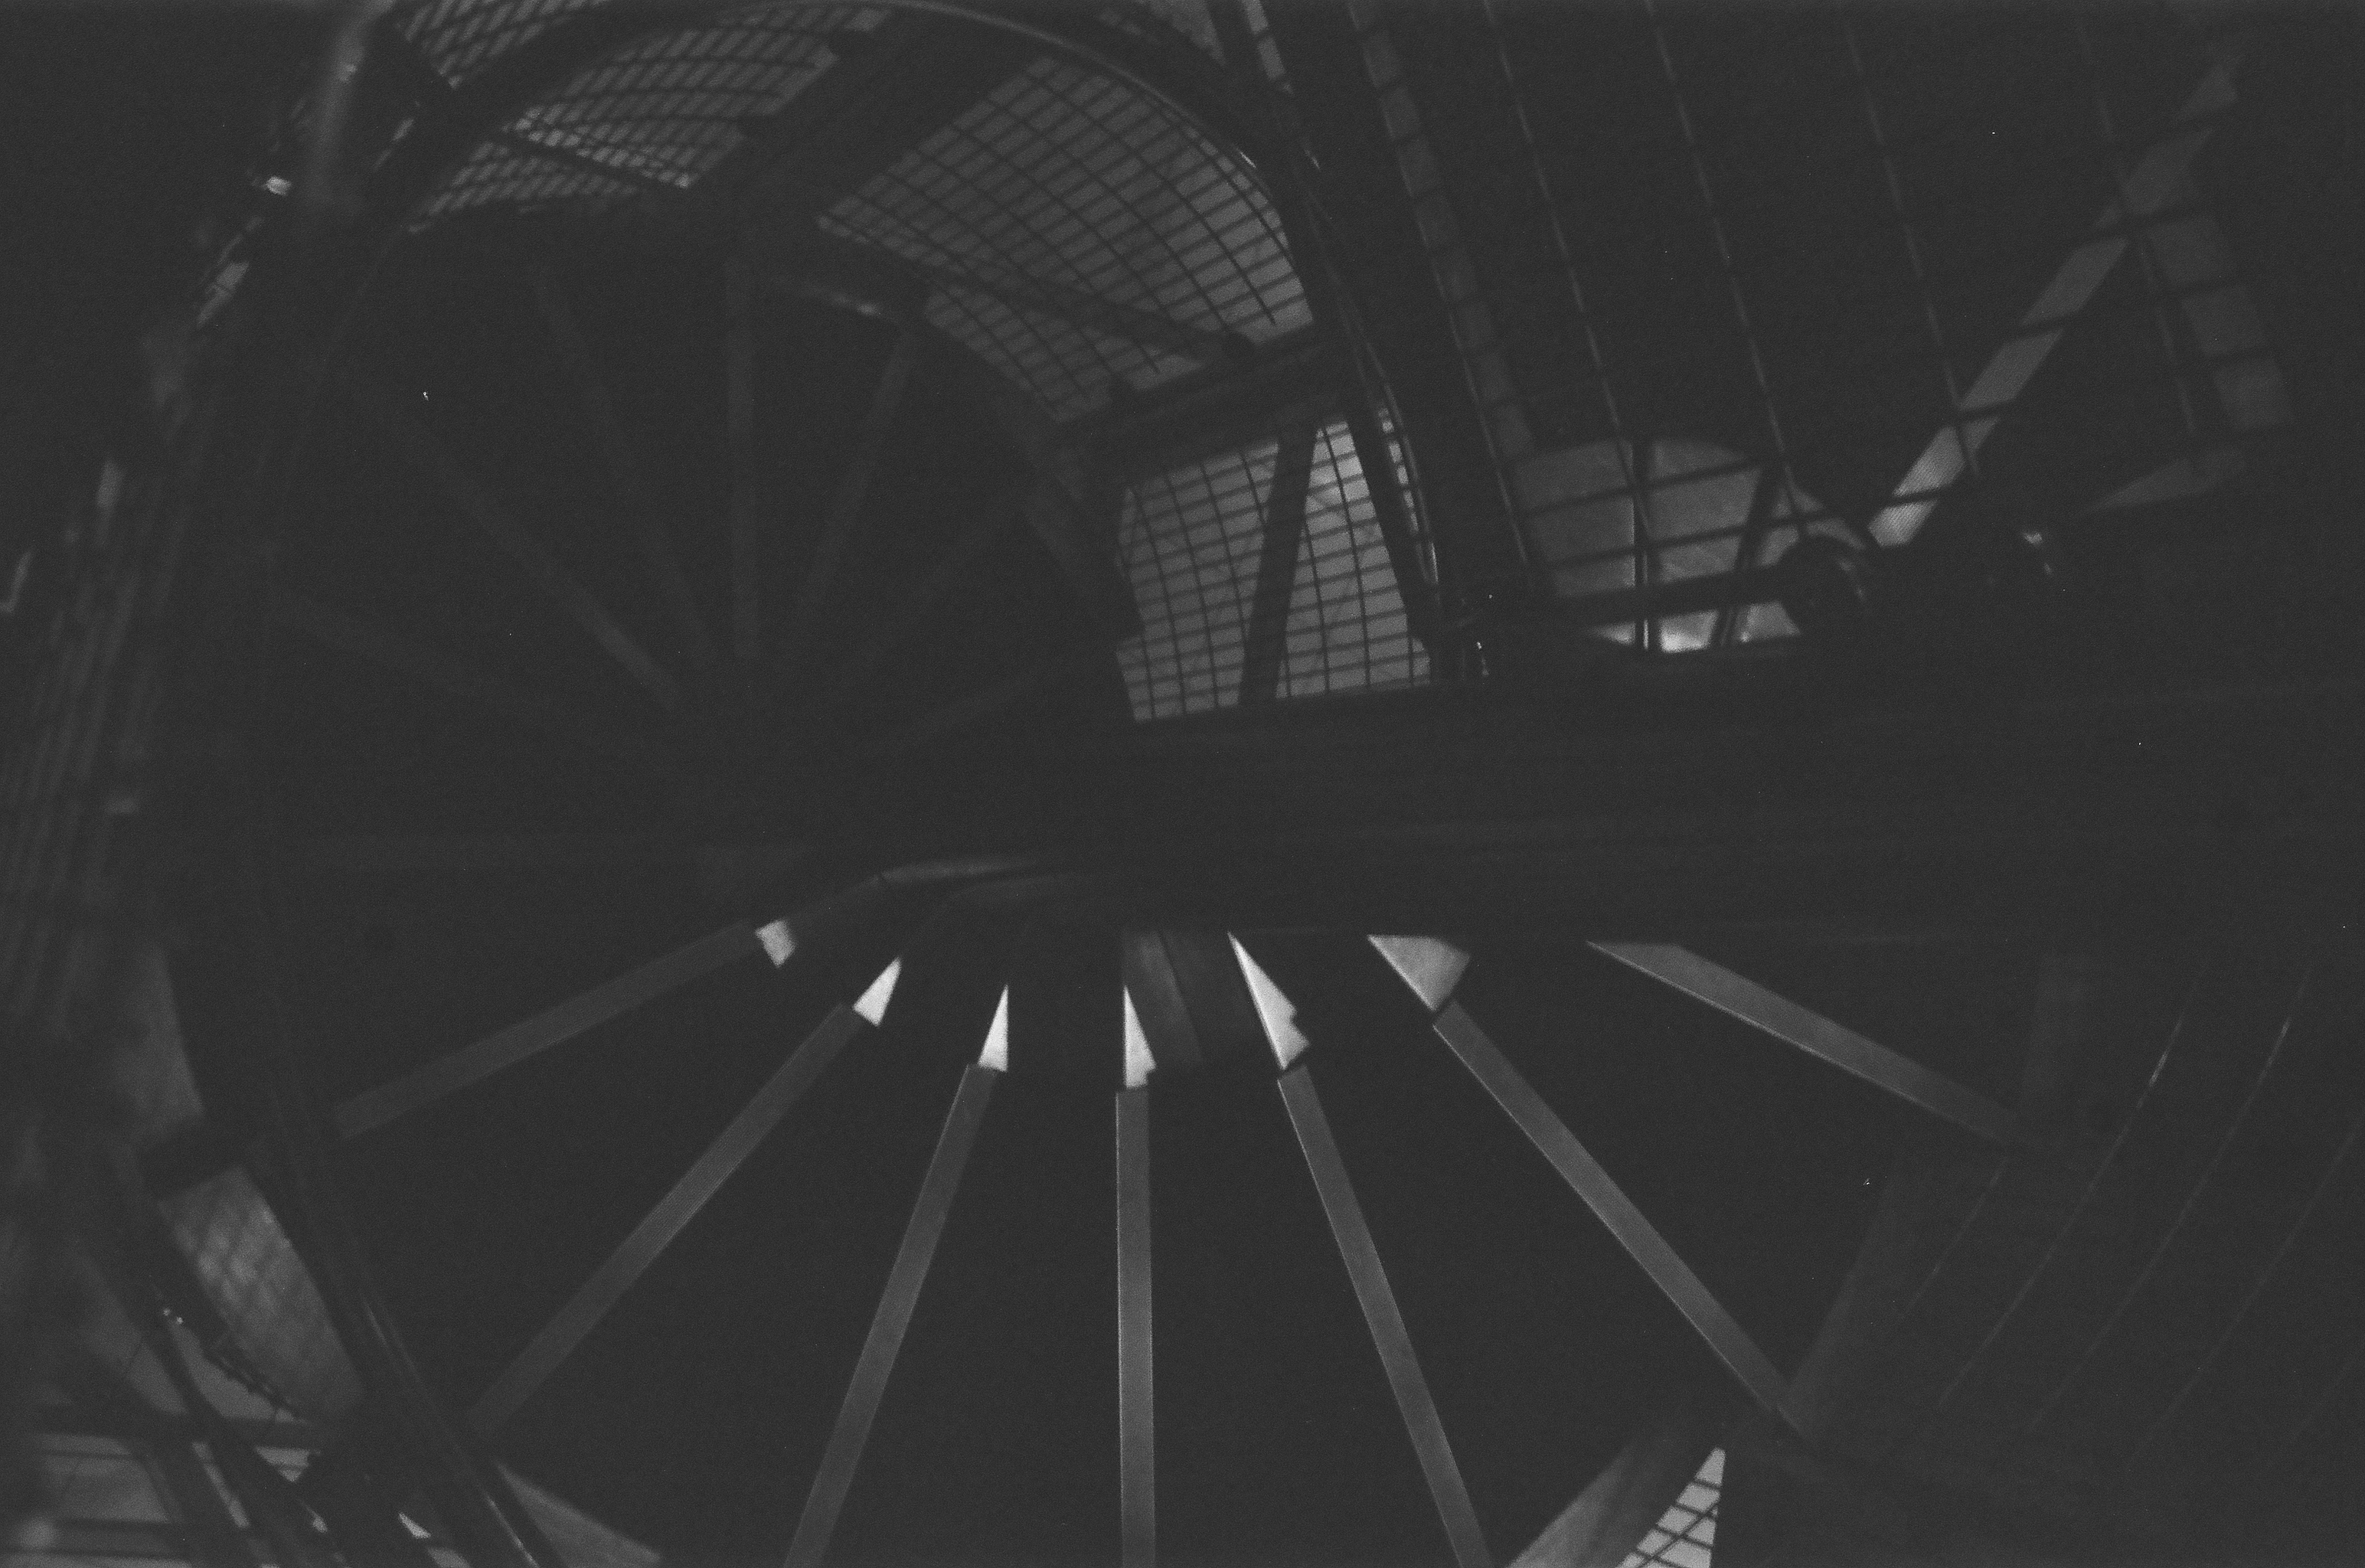
\includegraphics[angle=90, width=\linewidth, keepaspectratio]{Photos1/photos/analog11.jpg}
    \caption{Zdjęcie niedoświetlone}
\end{figure}
\begin{figure}[H]
    \centering
    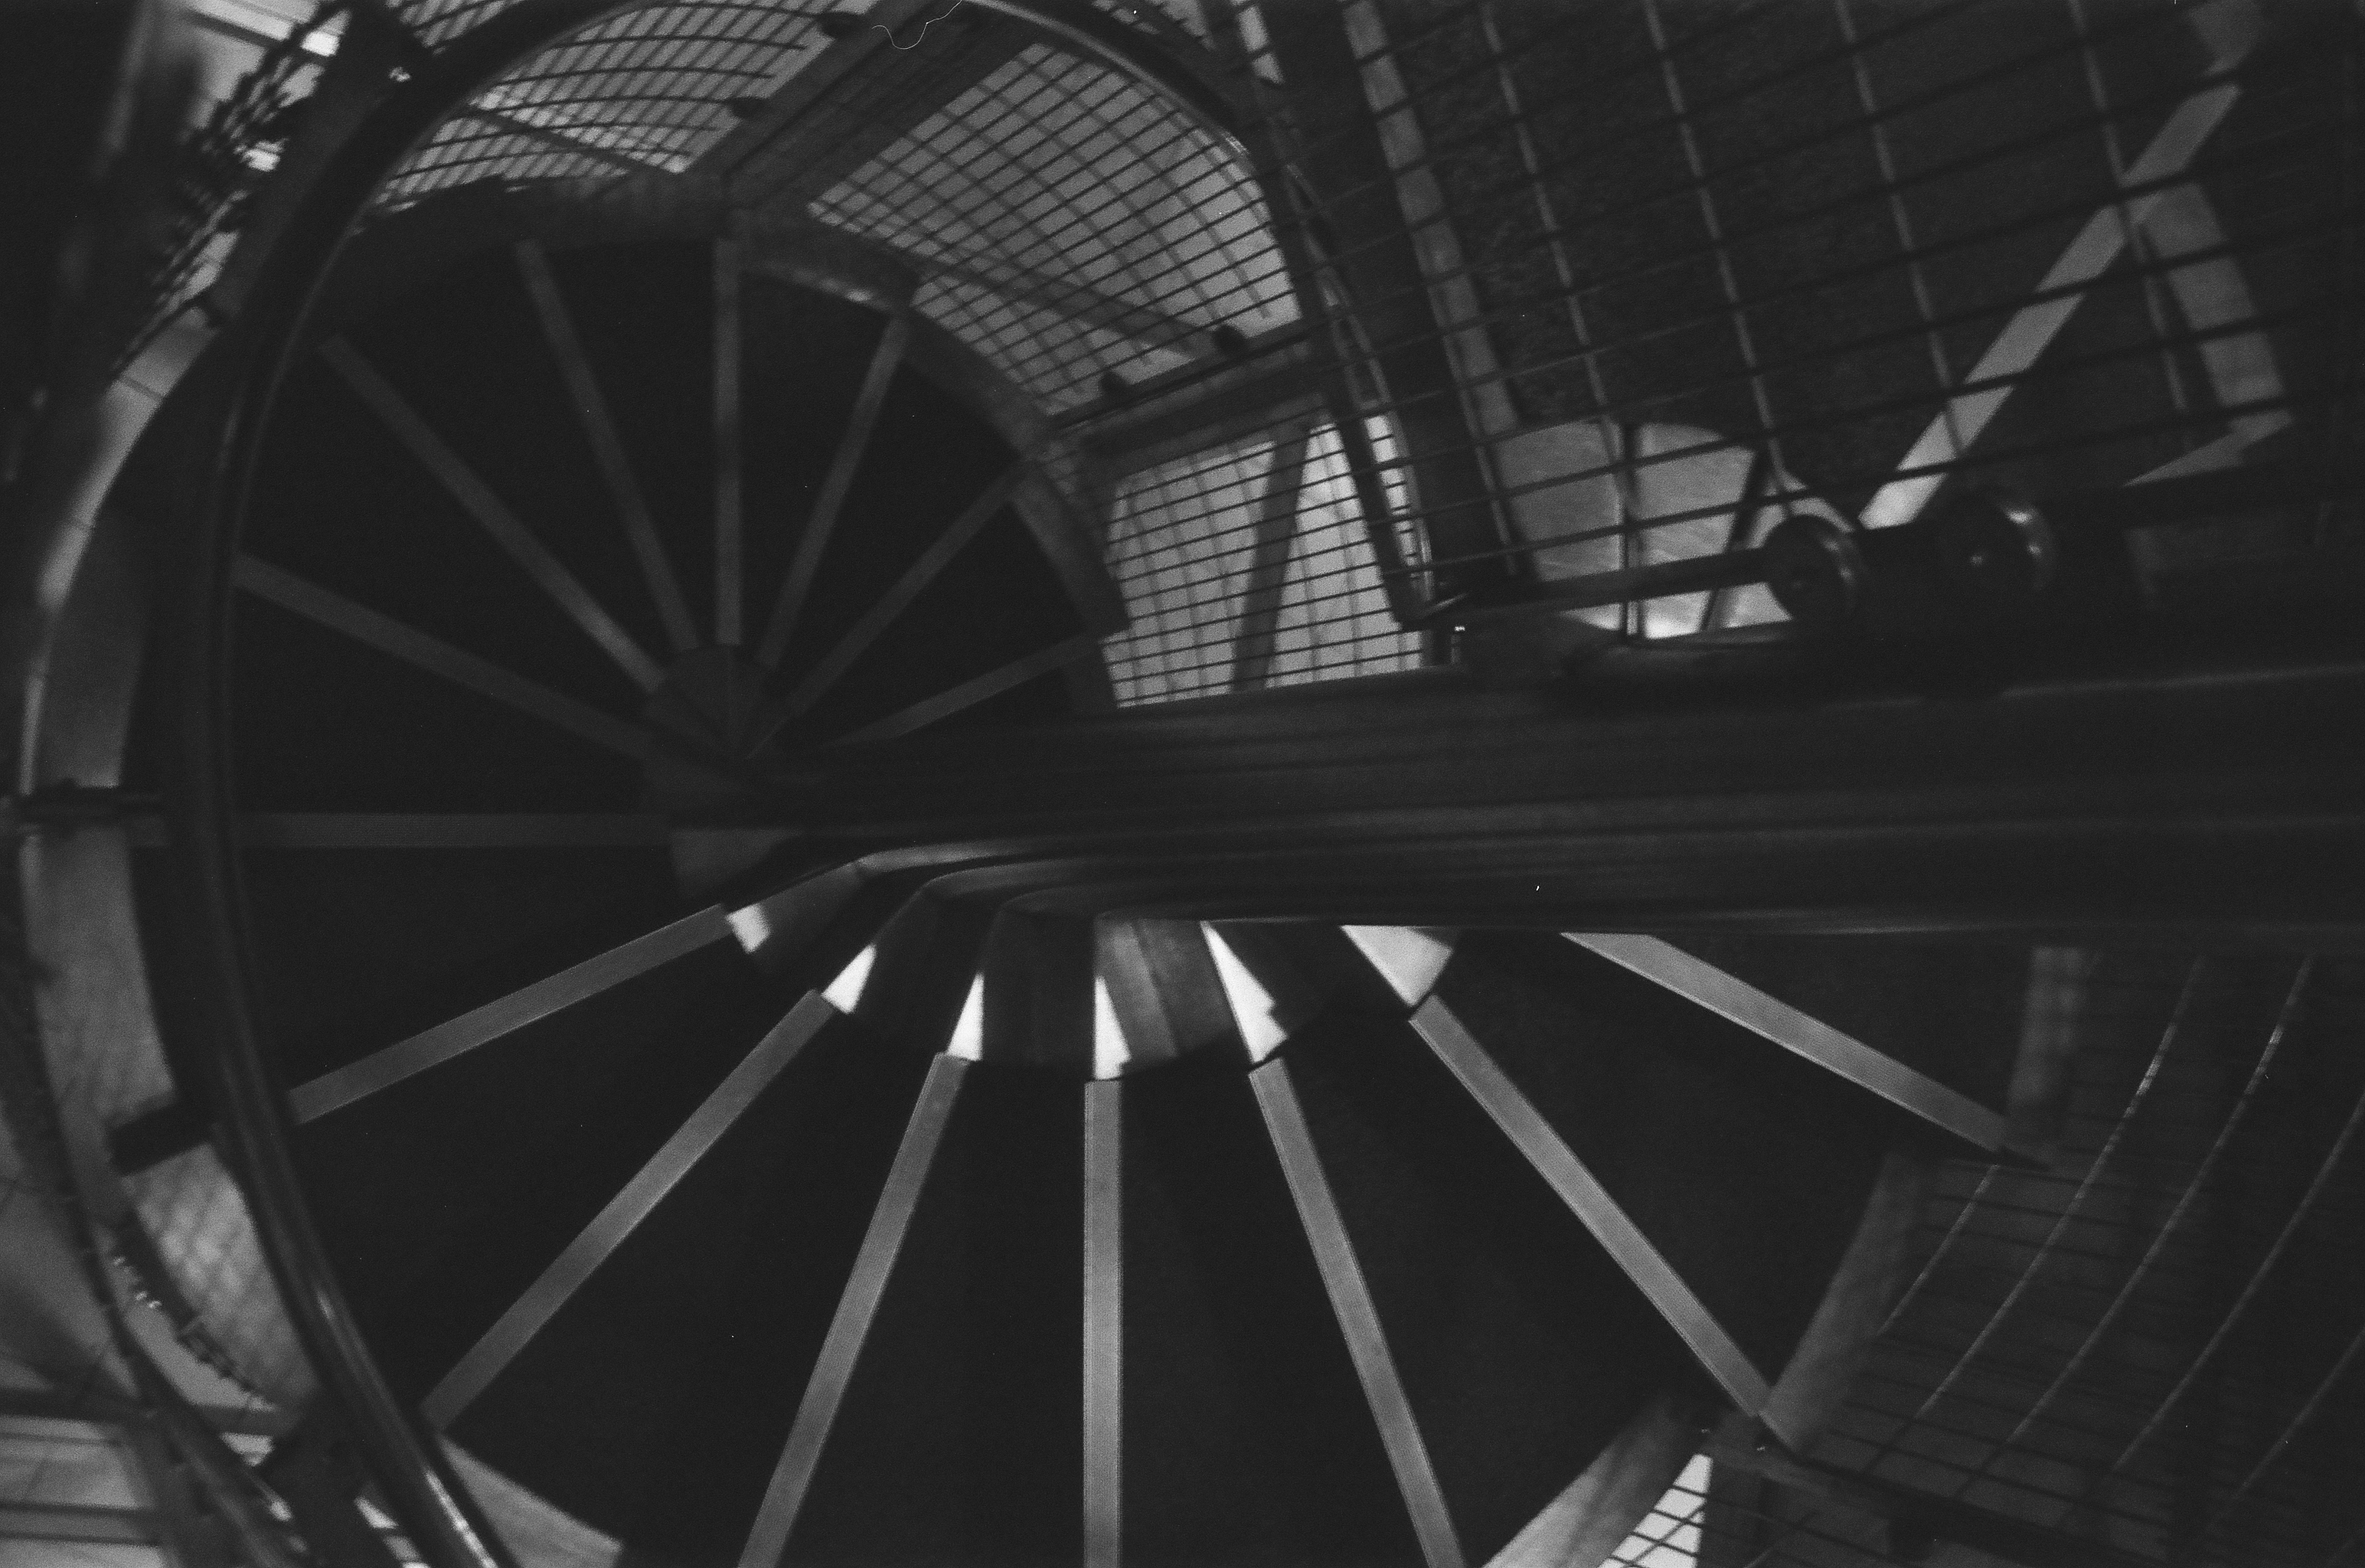
\includegraphics[angle=90, width=\linewidth, keepaspectratio]{Photos1/photos/analog14.jpg}
    \caption{Zdjęcie doświetlone}
\end{figure}



\begin{figure}[H]
    \centering
    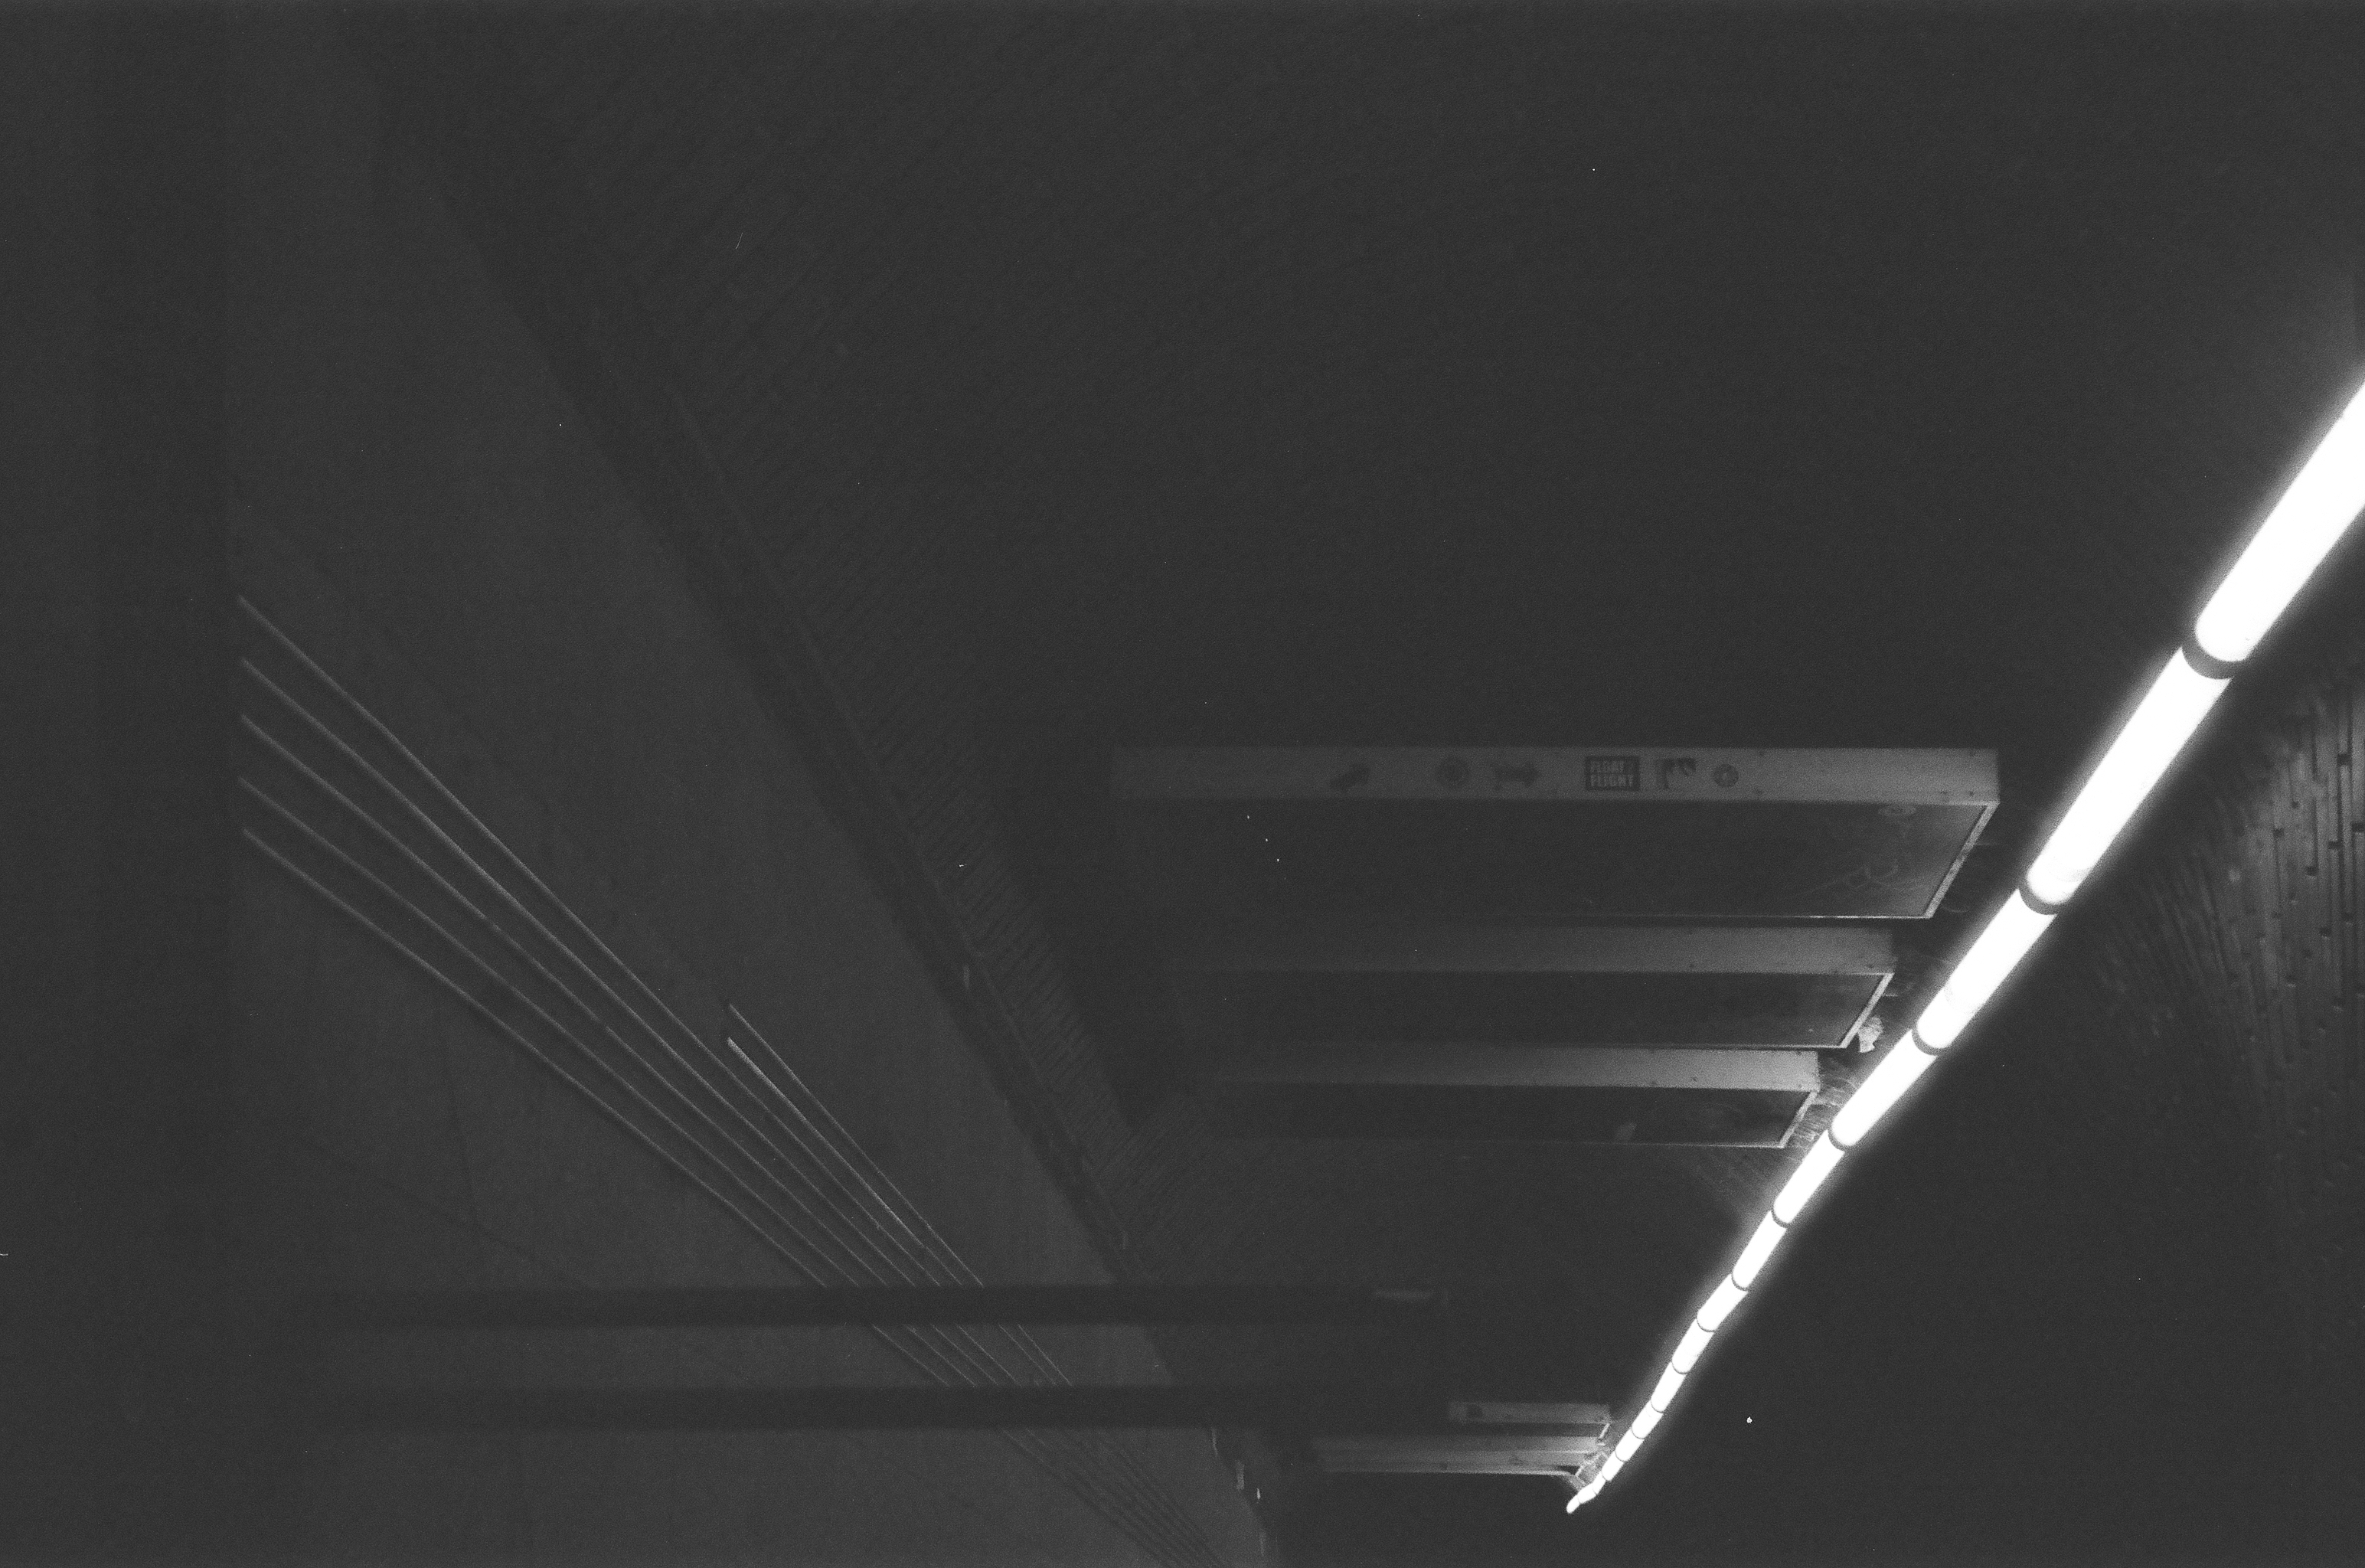
\includegraphics[angle=90, width=\linewidth, keepaspectratio]{Photos1/photos/analog23.jpg}
    \caption{Zdjęcie niedoświetlone}
\end{figure}
\begin{figure}[H]
    \centering
    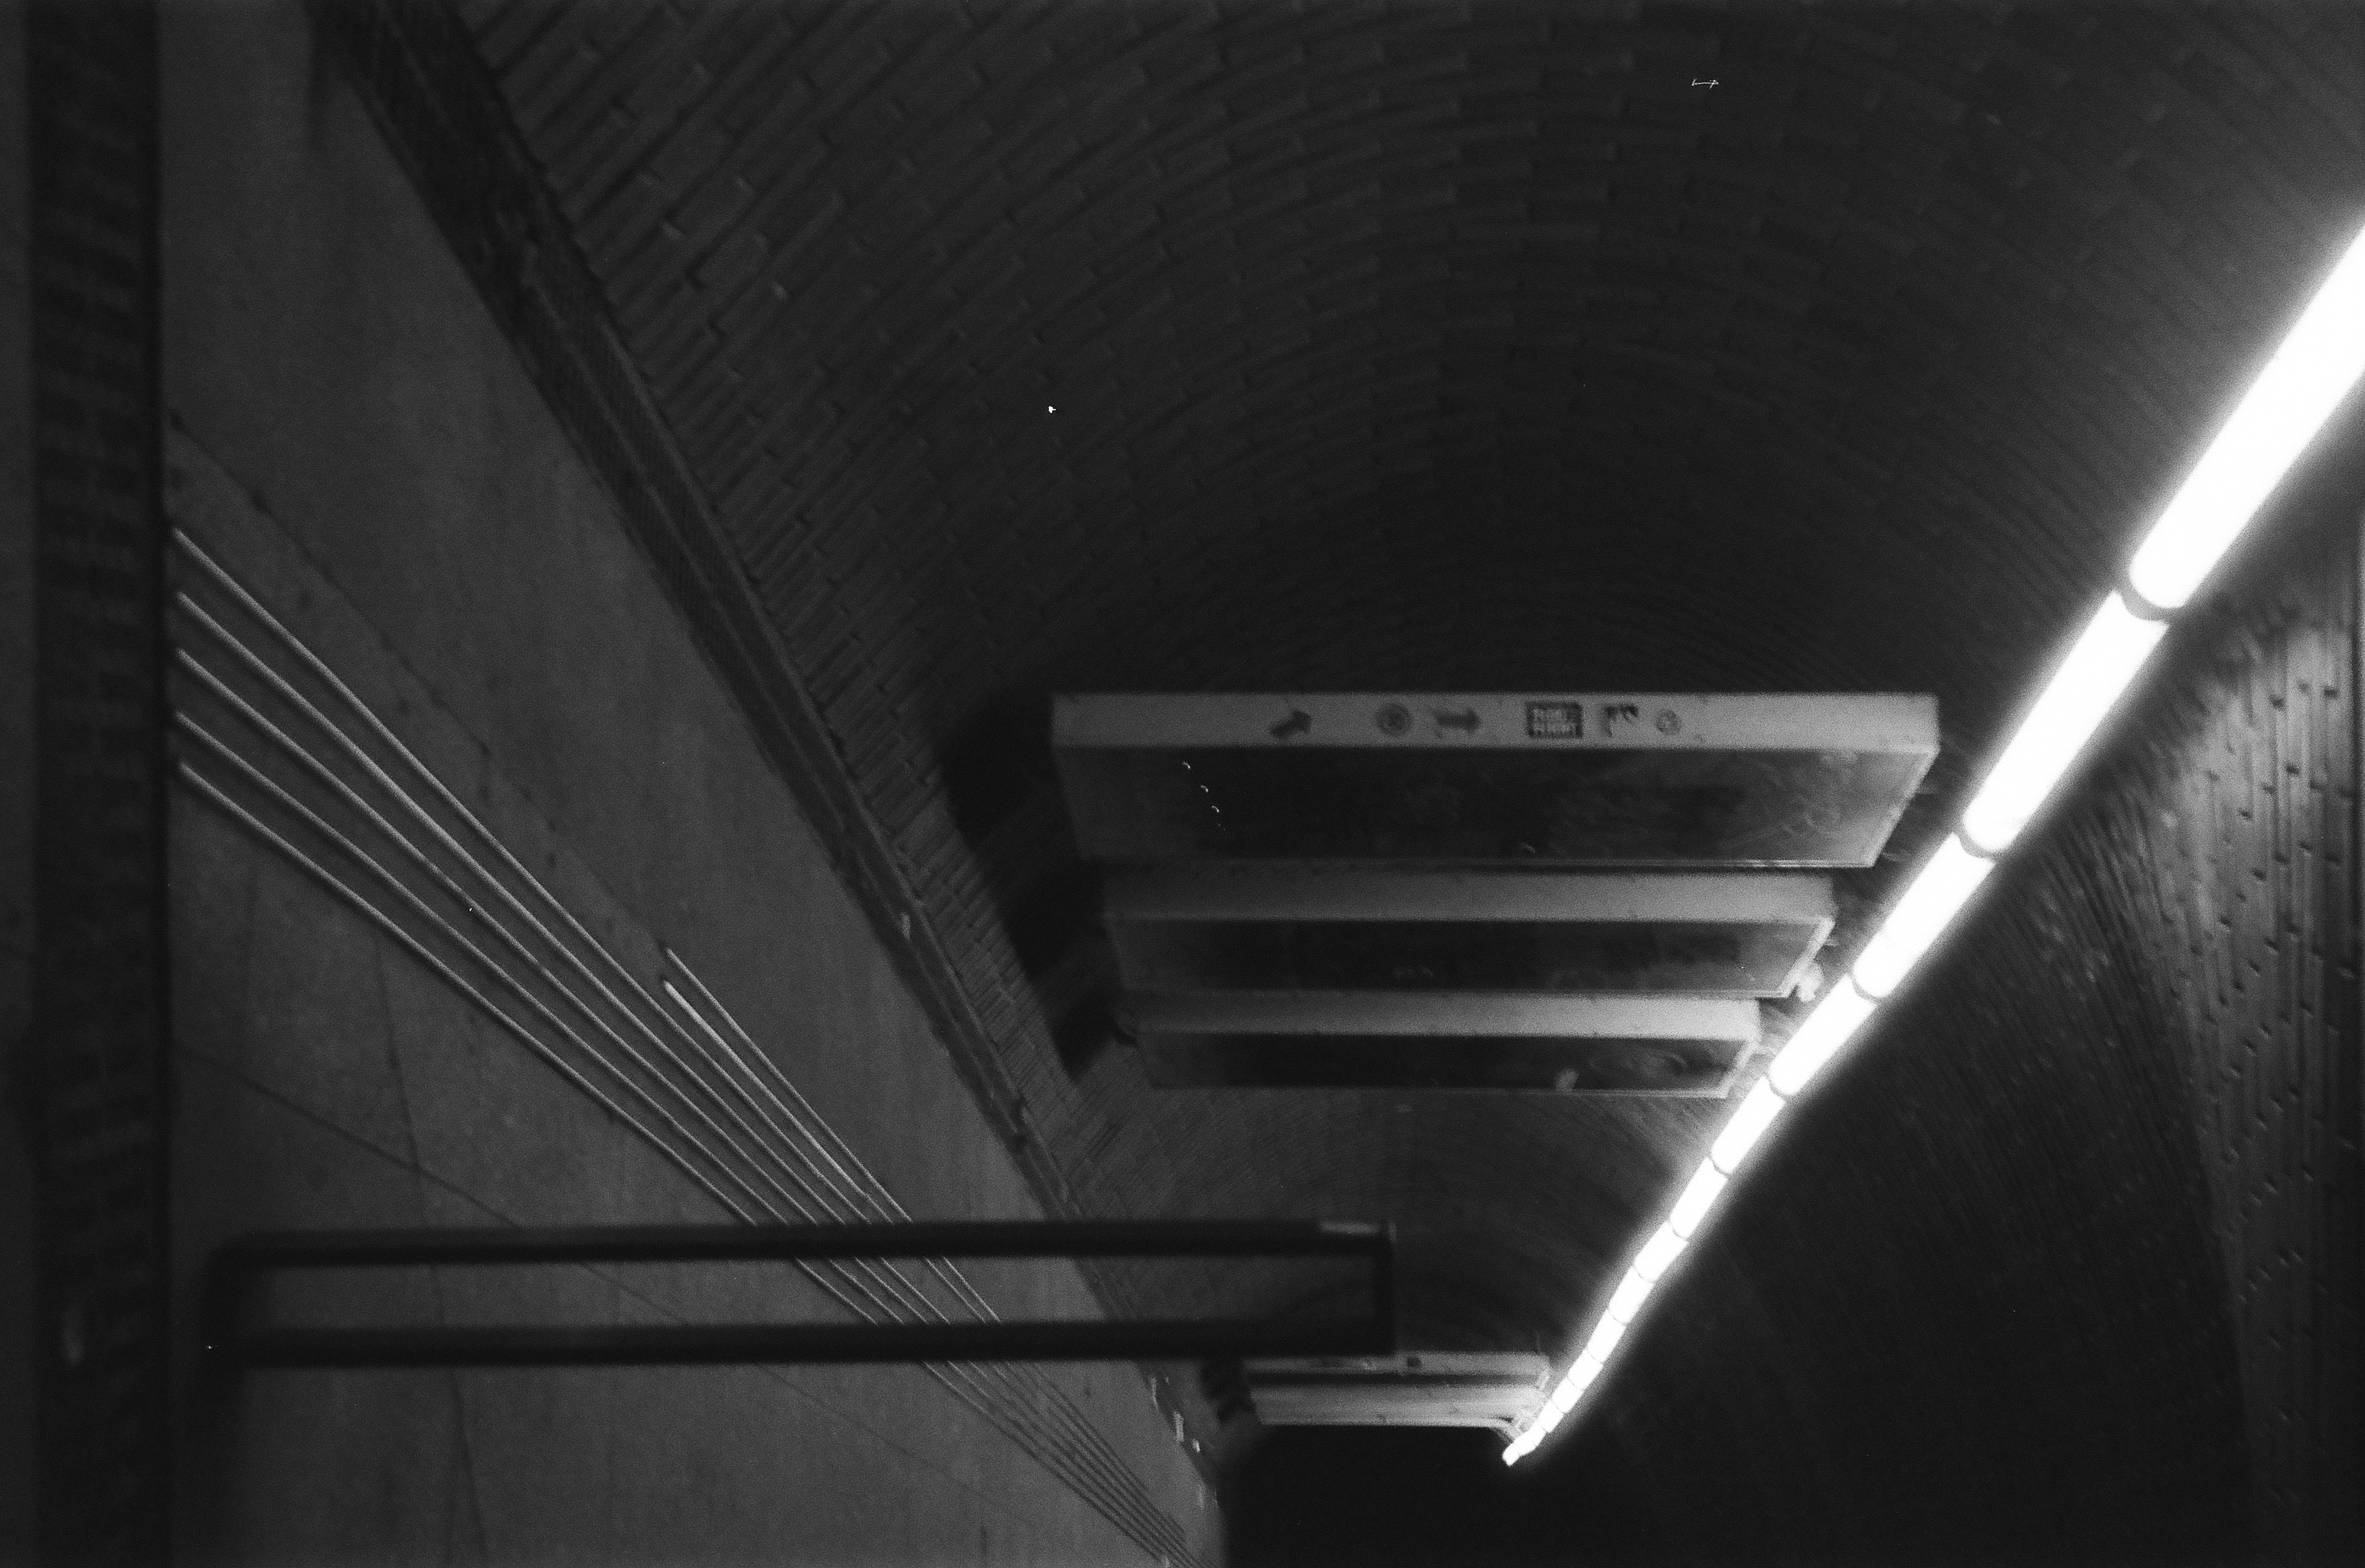
\includegraphics[angle=90, width=\linewidth, keepaspectratio]{Photos1/photos/analog22.jpg}
    \caption{Zdjęcie doświetlone}
\end{figure}


\begin{figure}[H]
    \centering
    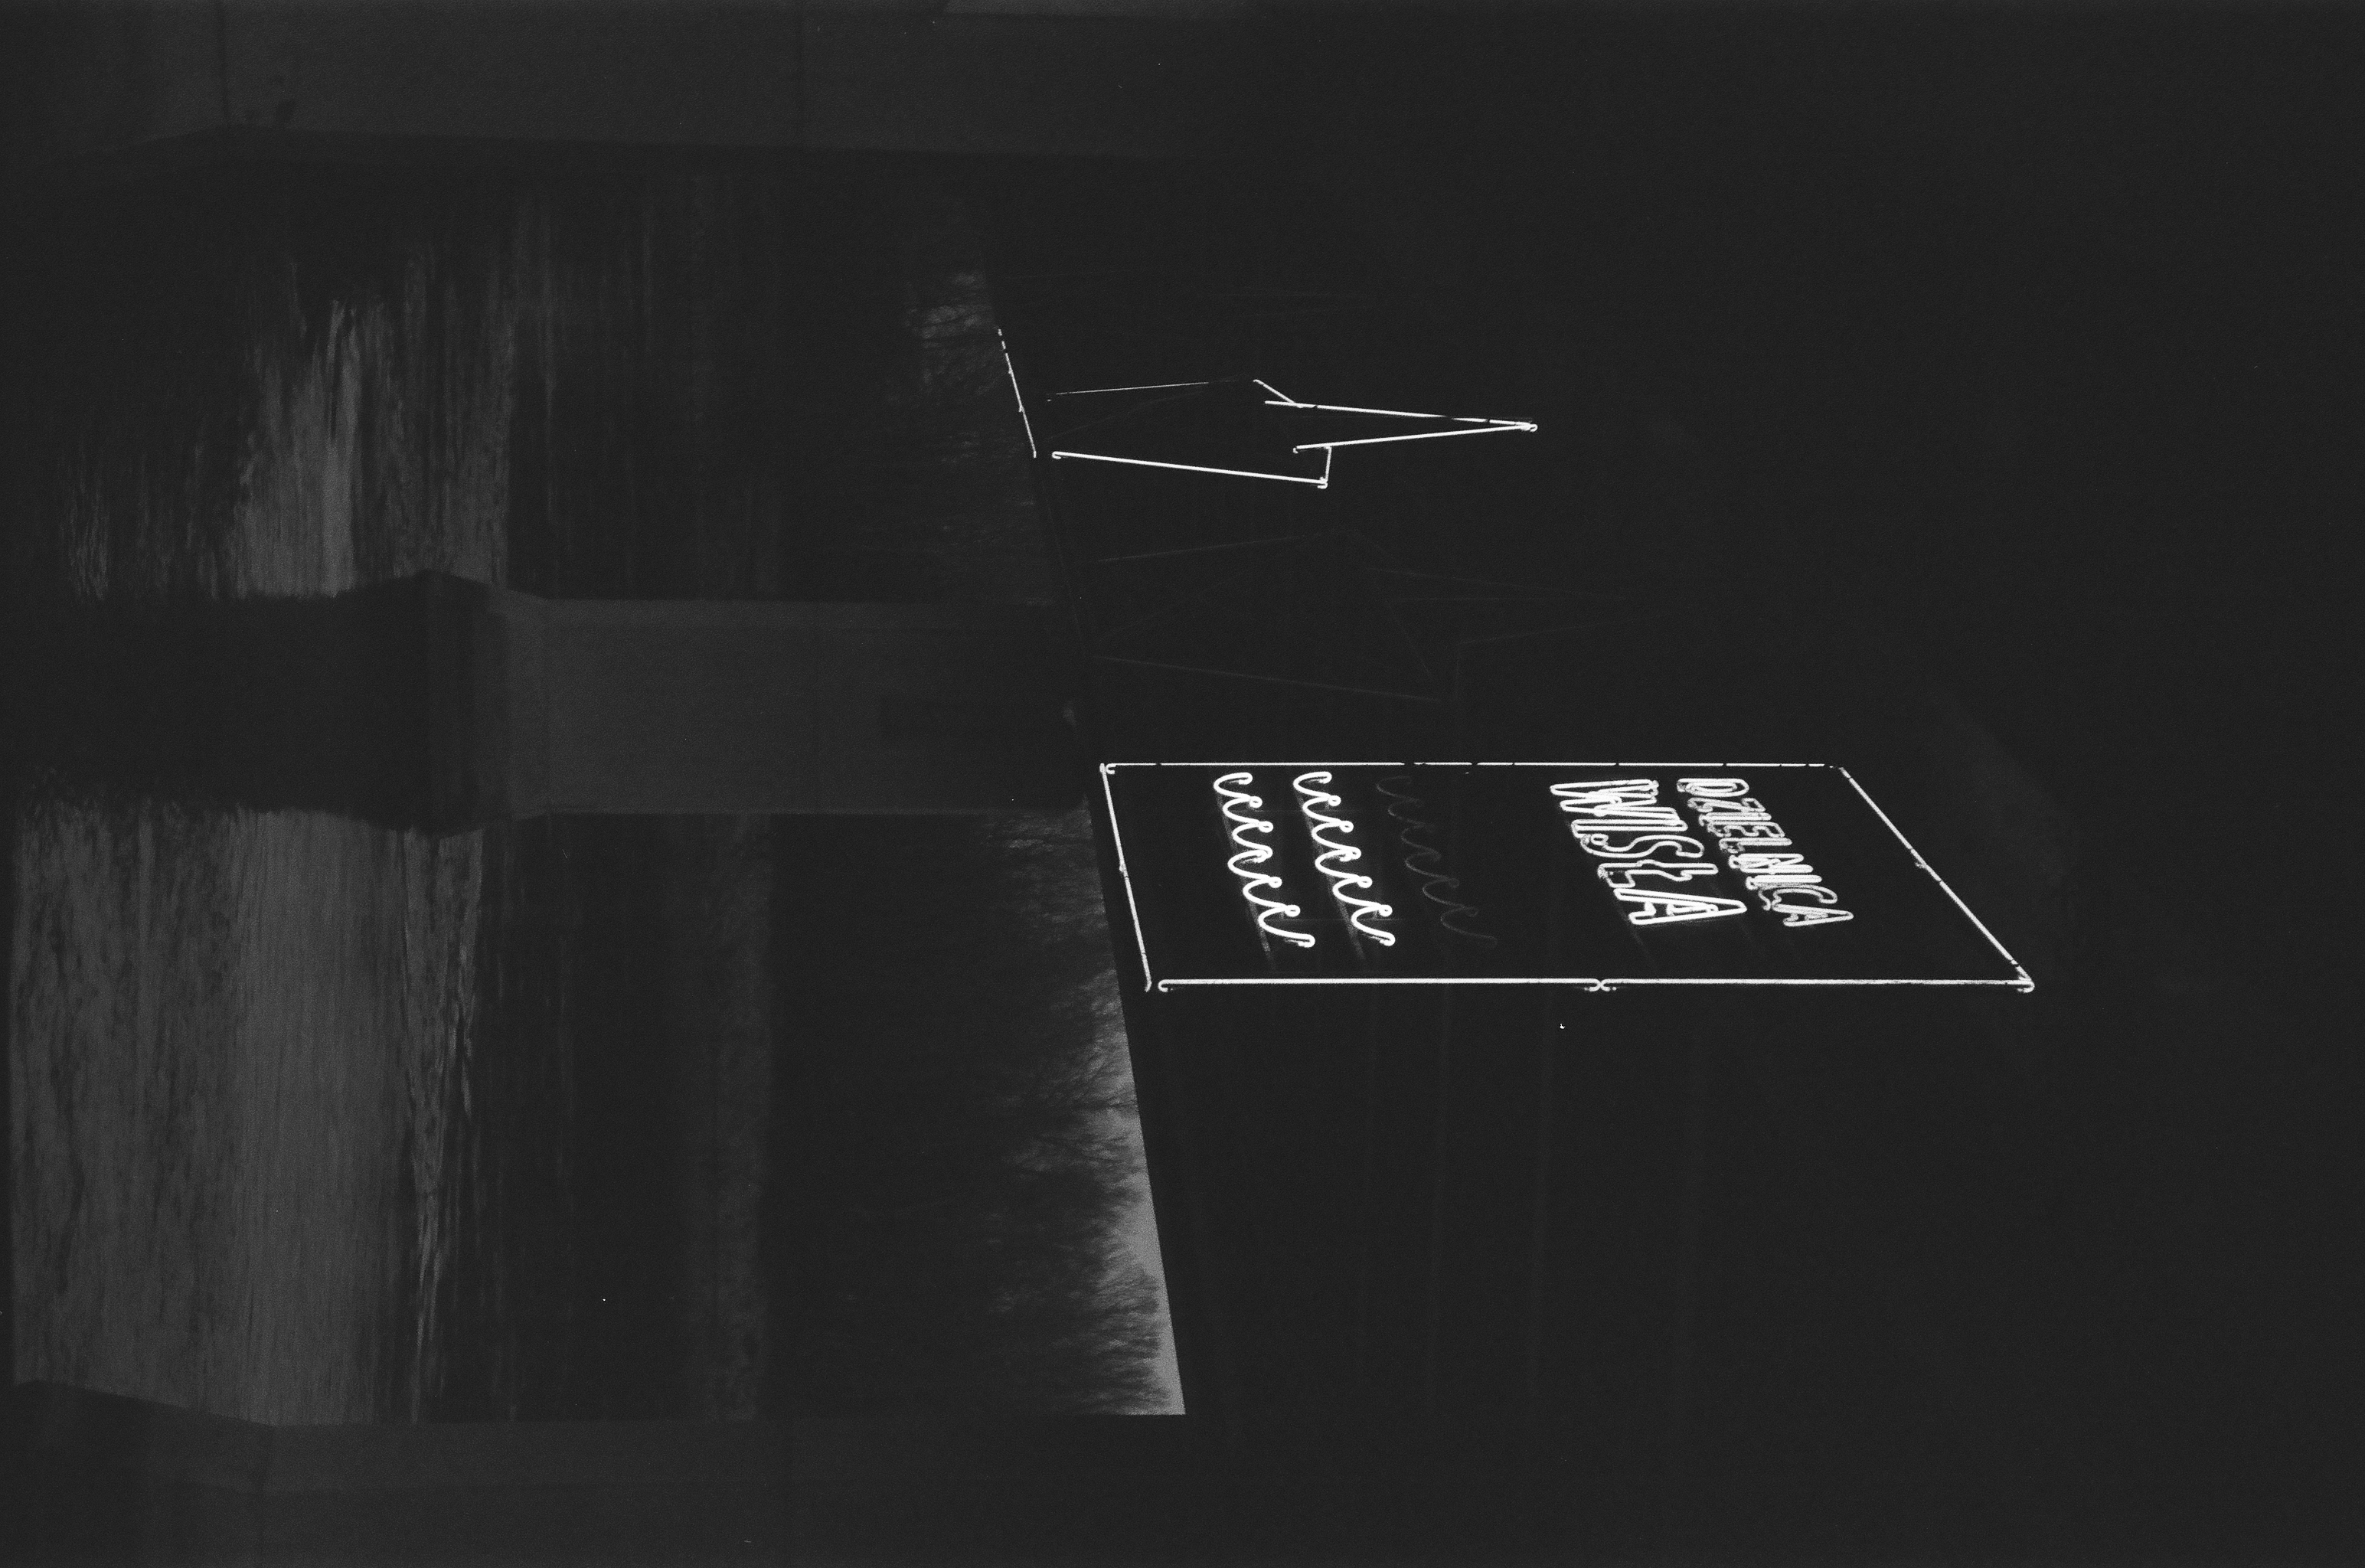
\includegraphics[angle=90, width=\linewidth, keepaspectratio]{Photos1/photos/analog35.jpg}
    \caption{Zdjęcie niedoświetlone}
\end{figure}
\begin{figure}[H]
    \centering
    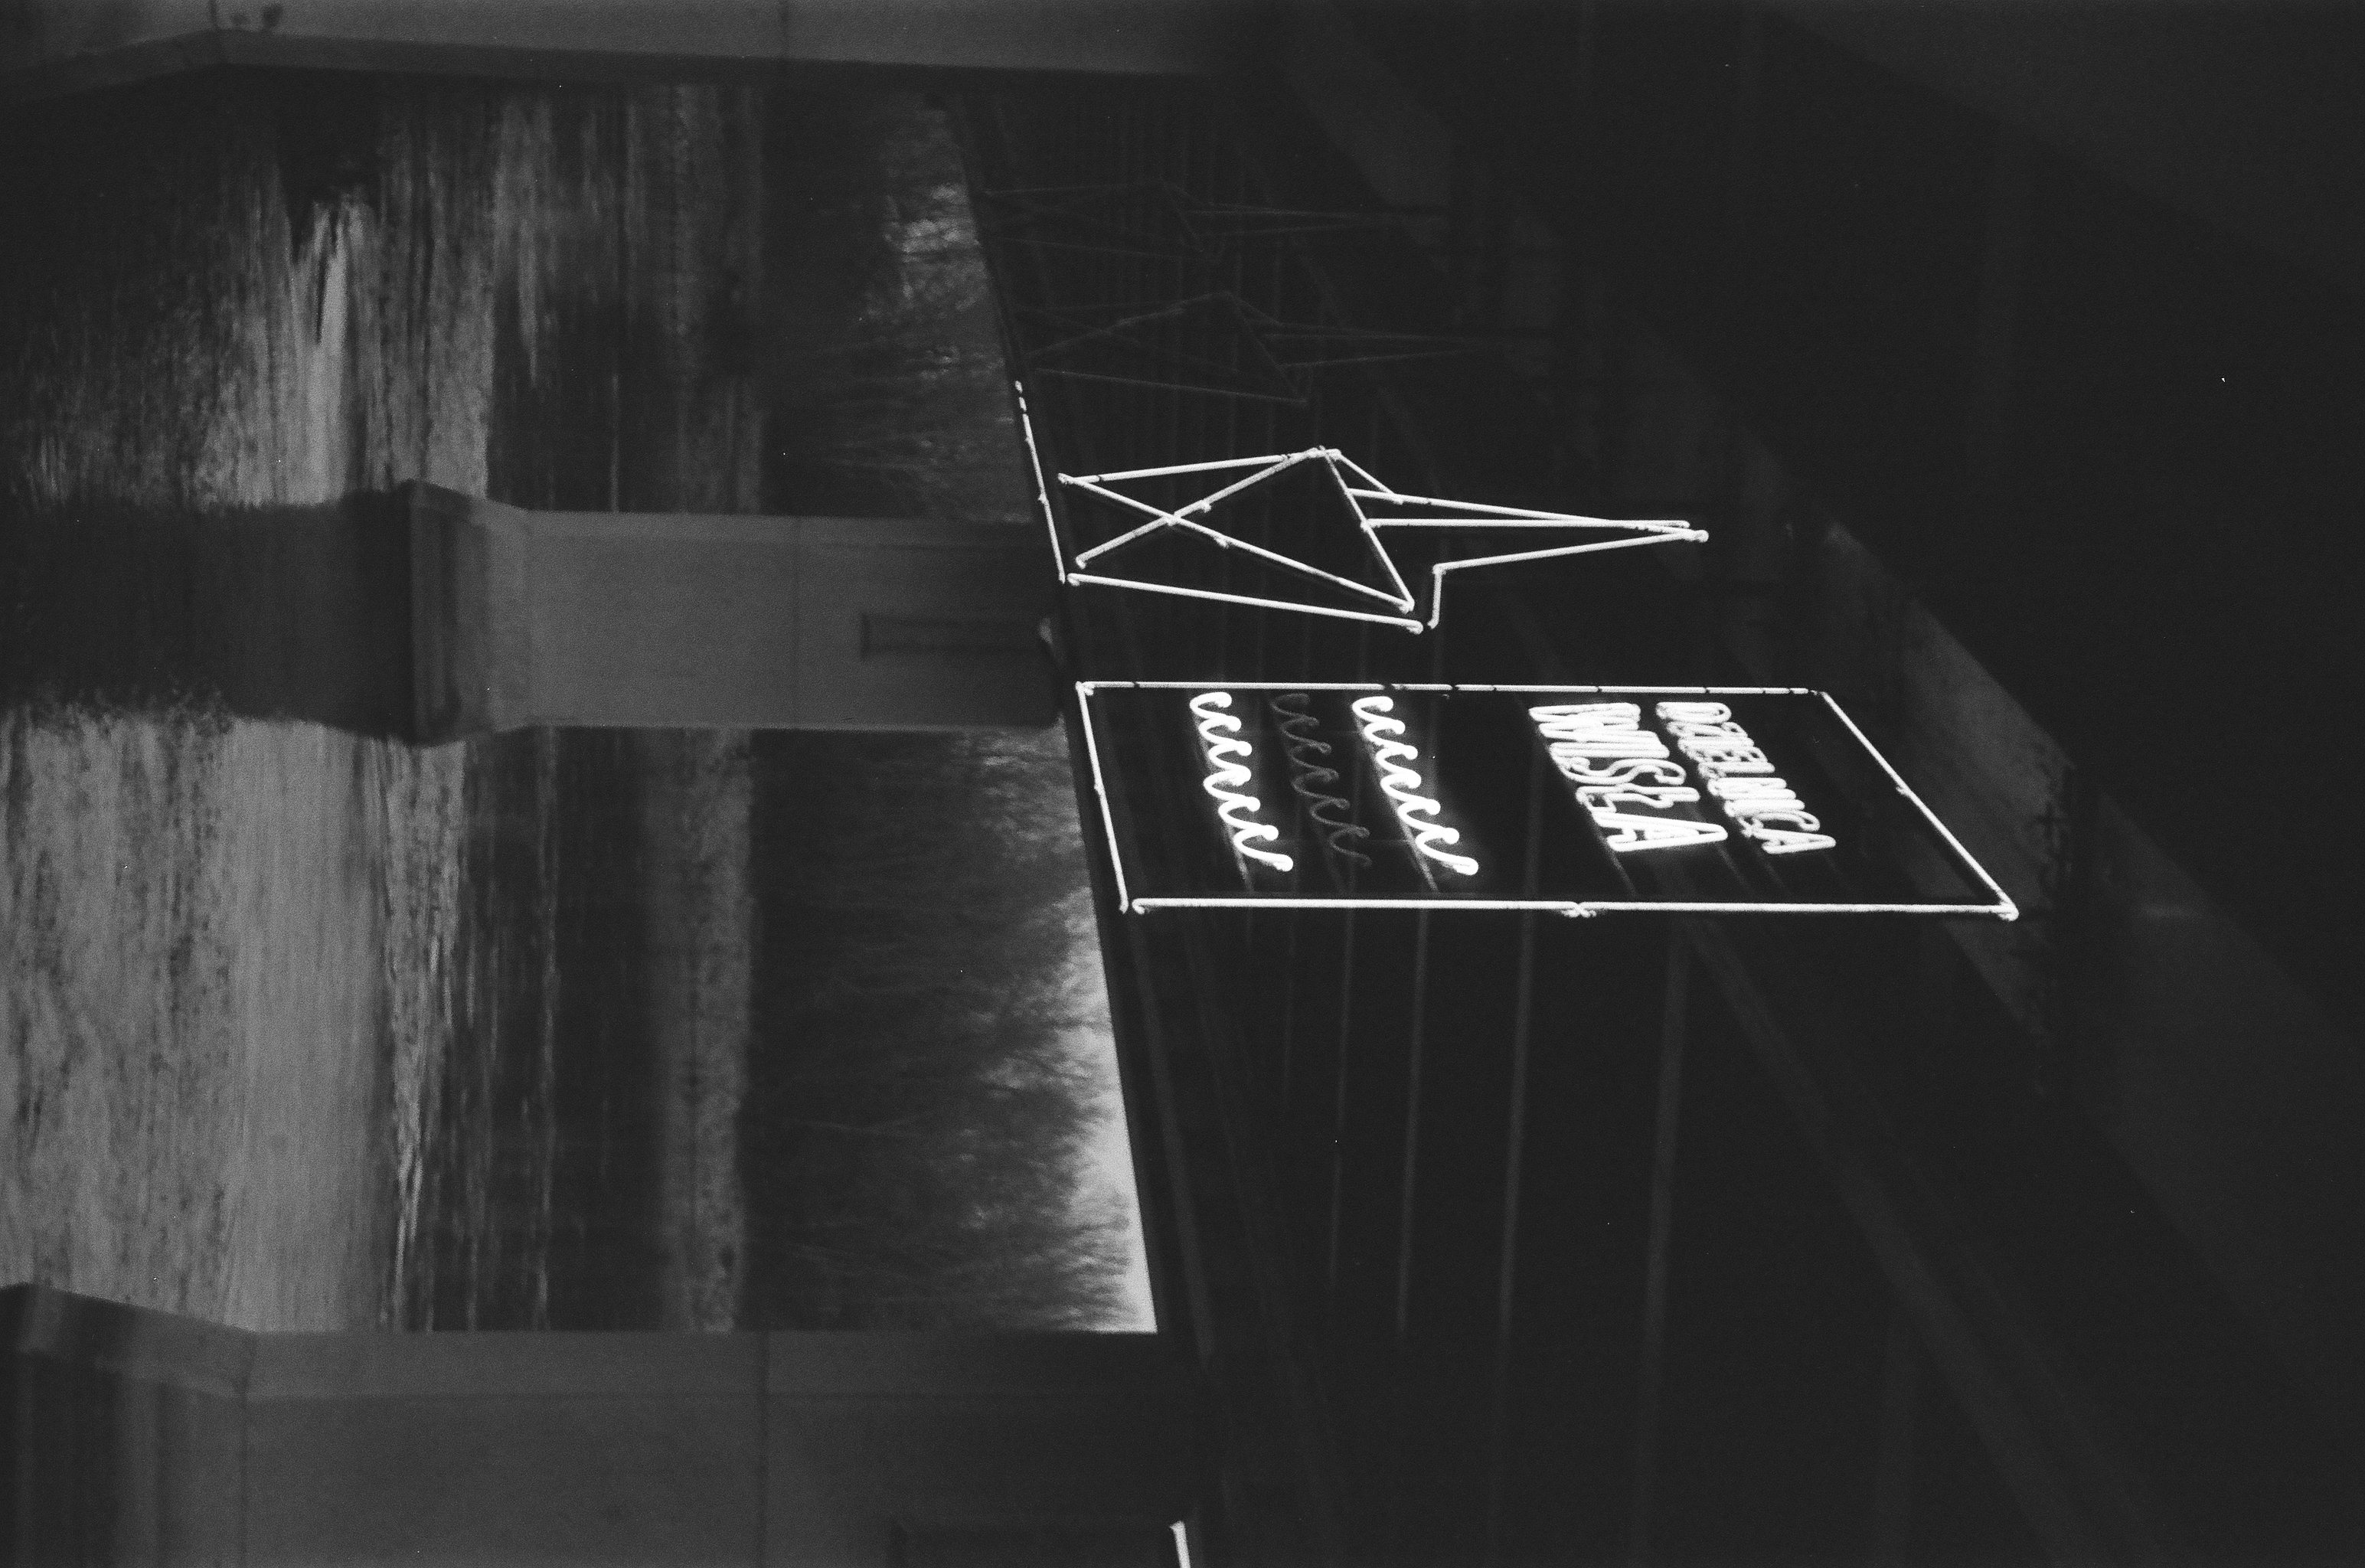
\includegraphics[angle=90, width=\linewidth, keepaspectratio]{Photos1/photos/analog36.jpg}
    \caption{Zdjęcie doświetlone}
\end{figure}


\newpage
A także w przypadku fotografii cyfrowej:

\begin{figure}[H]
    \centering
    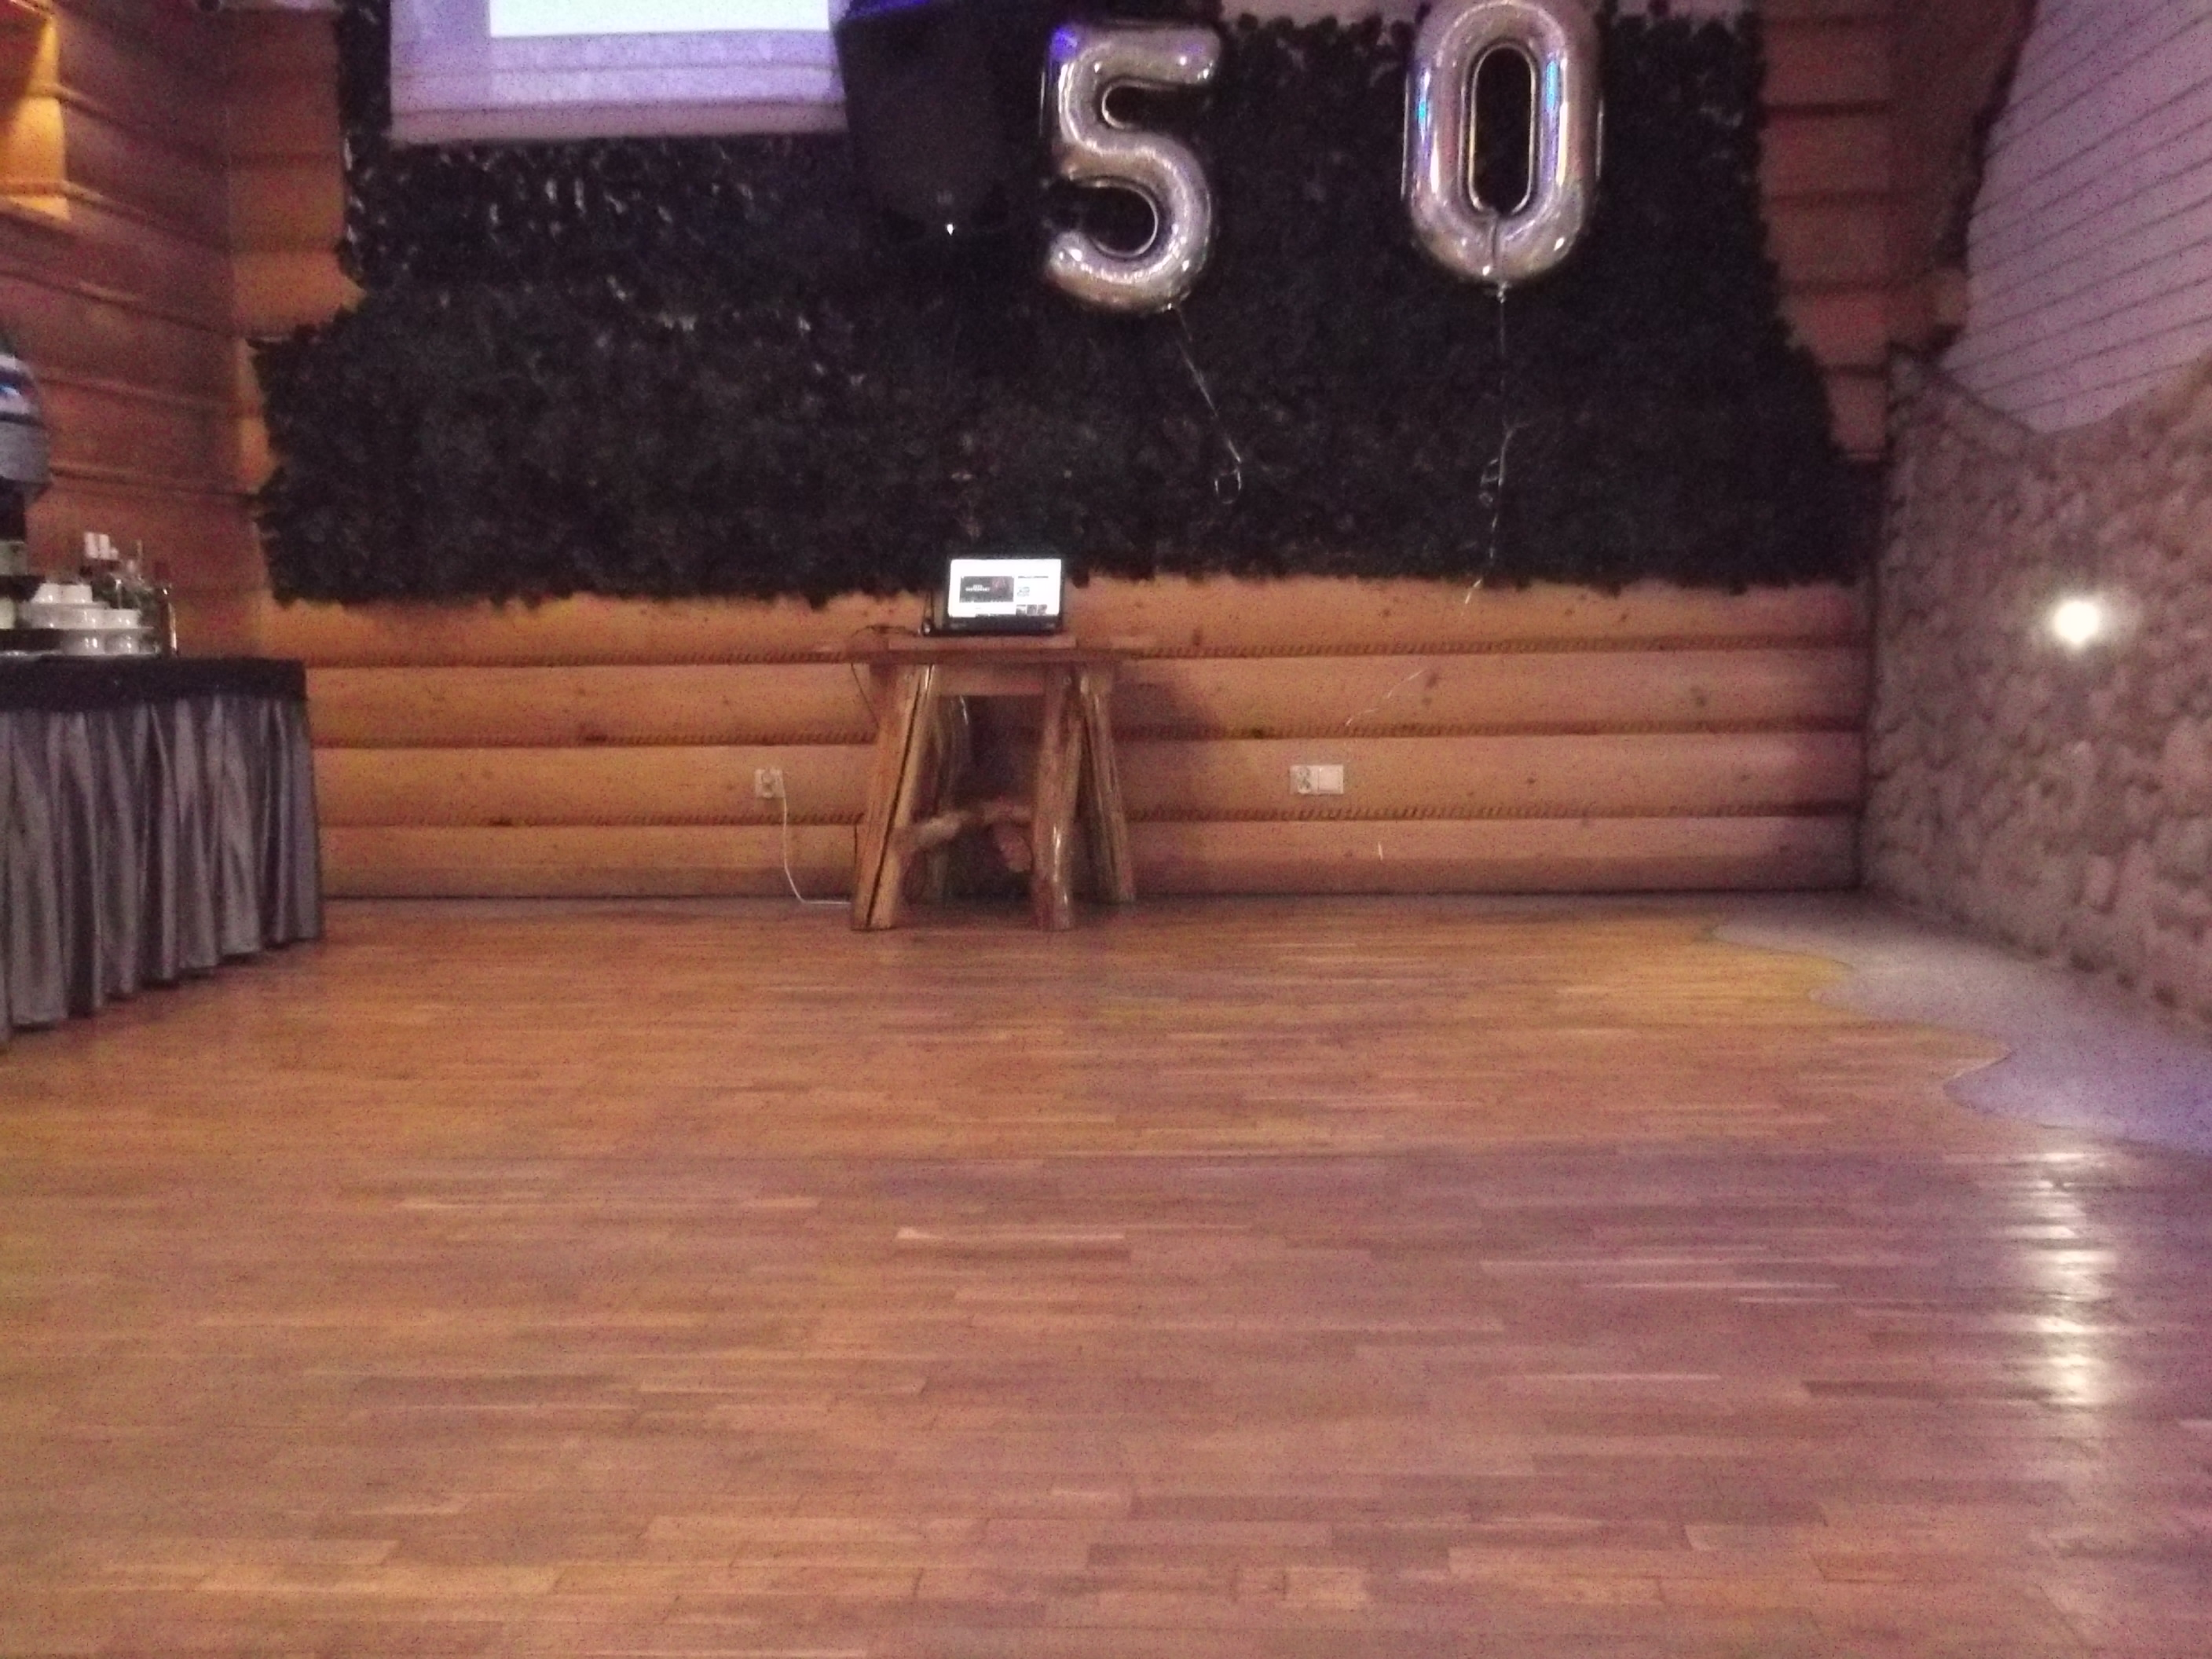
\includegraphics[width=\linewidth, keepaspectratio]{Photos1/photos/balony3.jpg}
    \caption{Zdjęcie niedoświetlone}
\end{figure}
\begin{figure}[H]
    \centering
    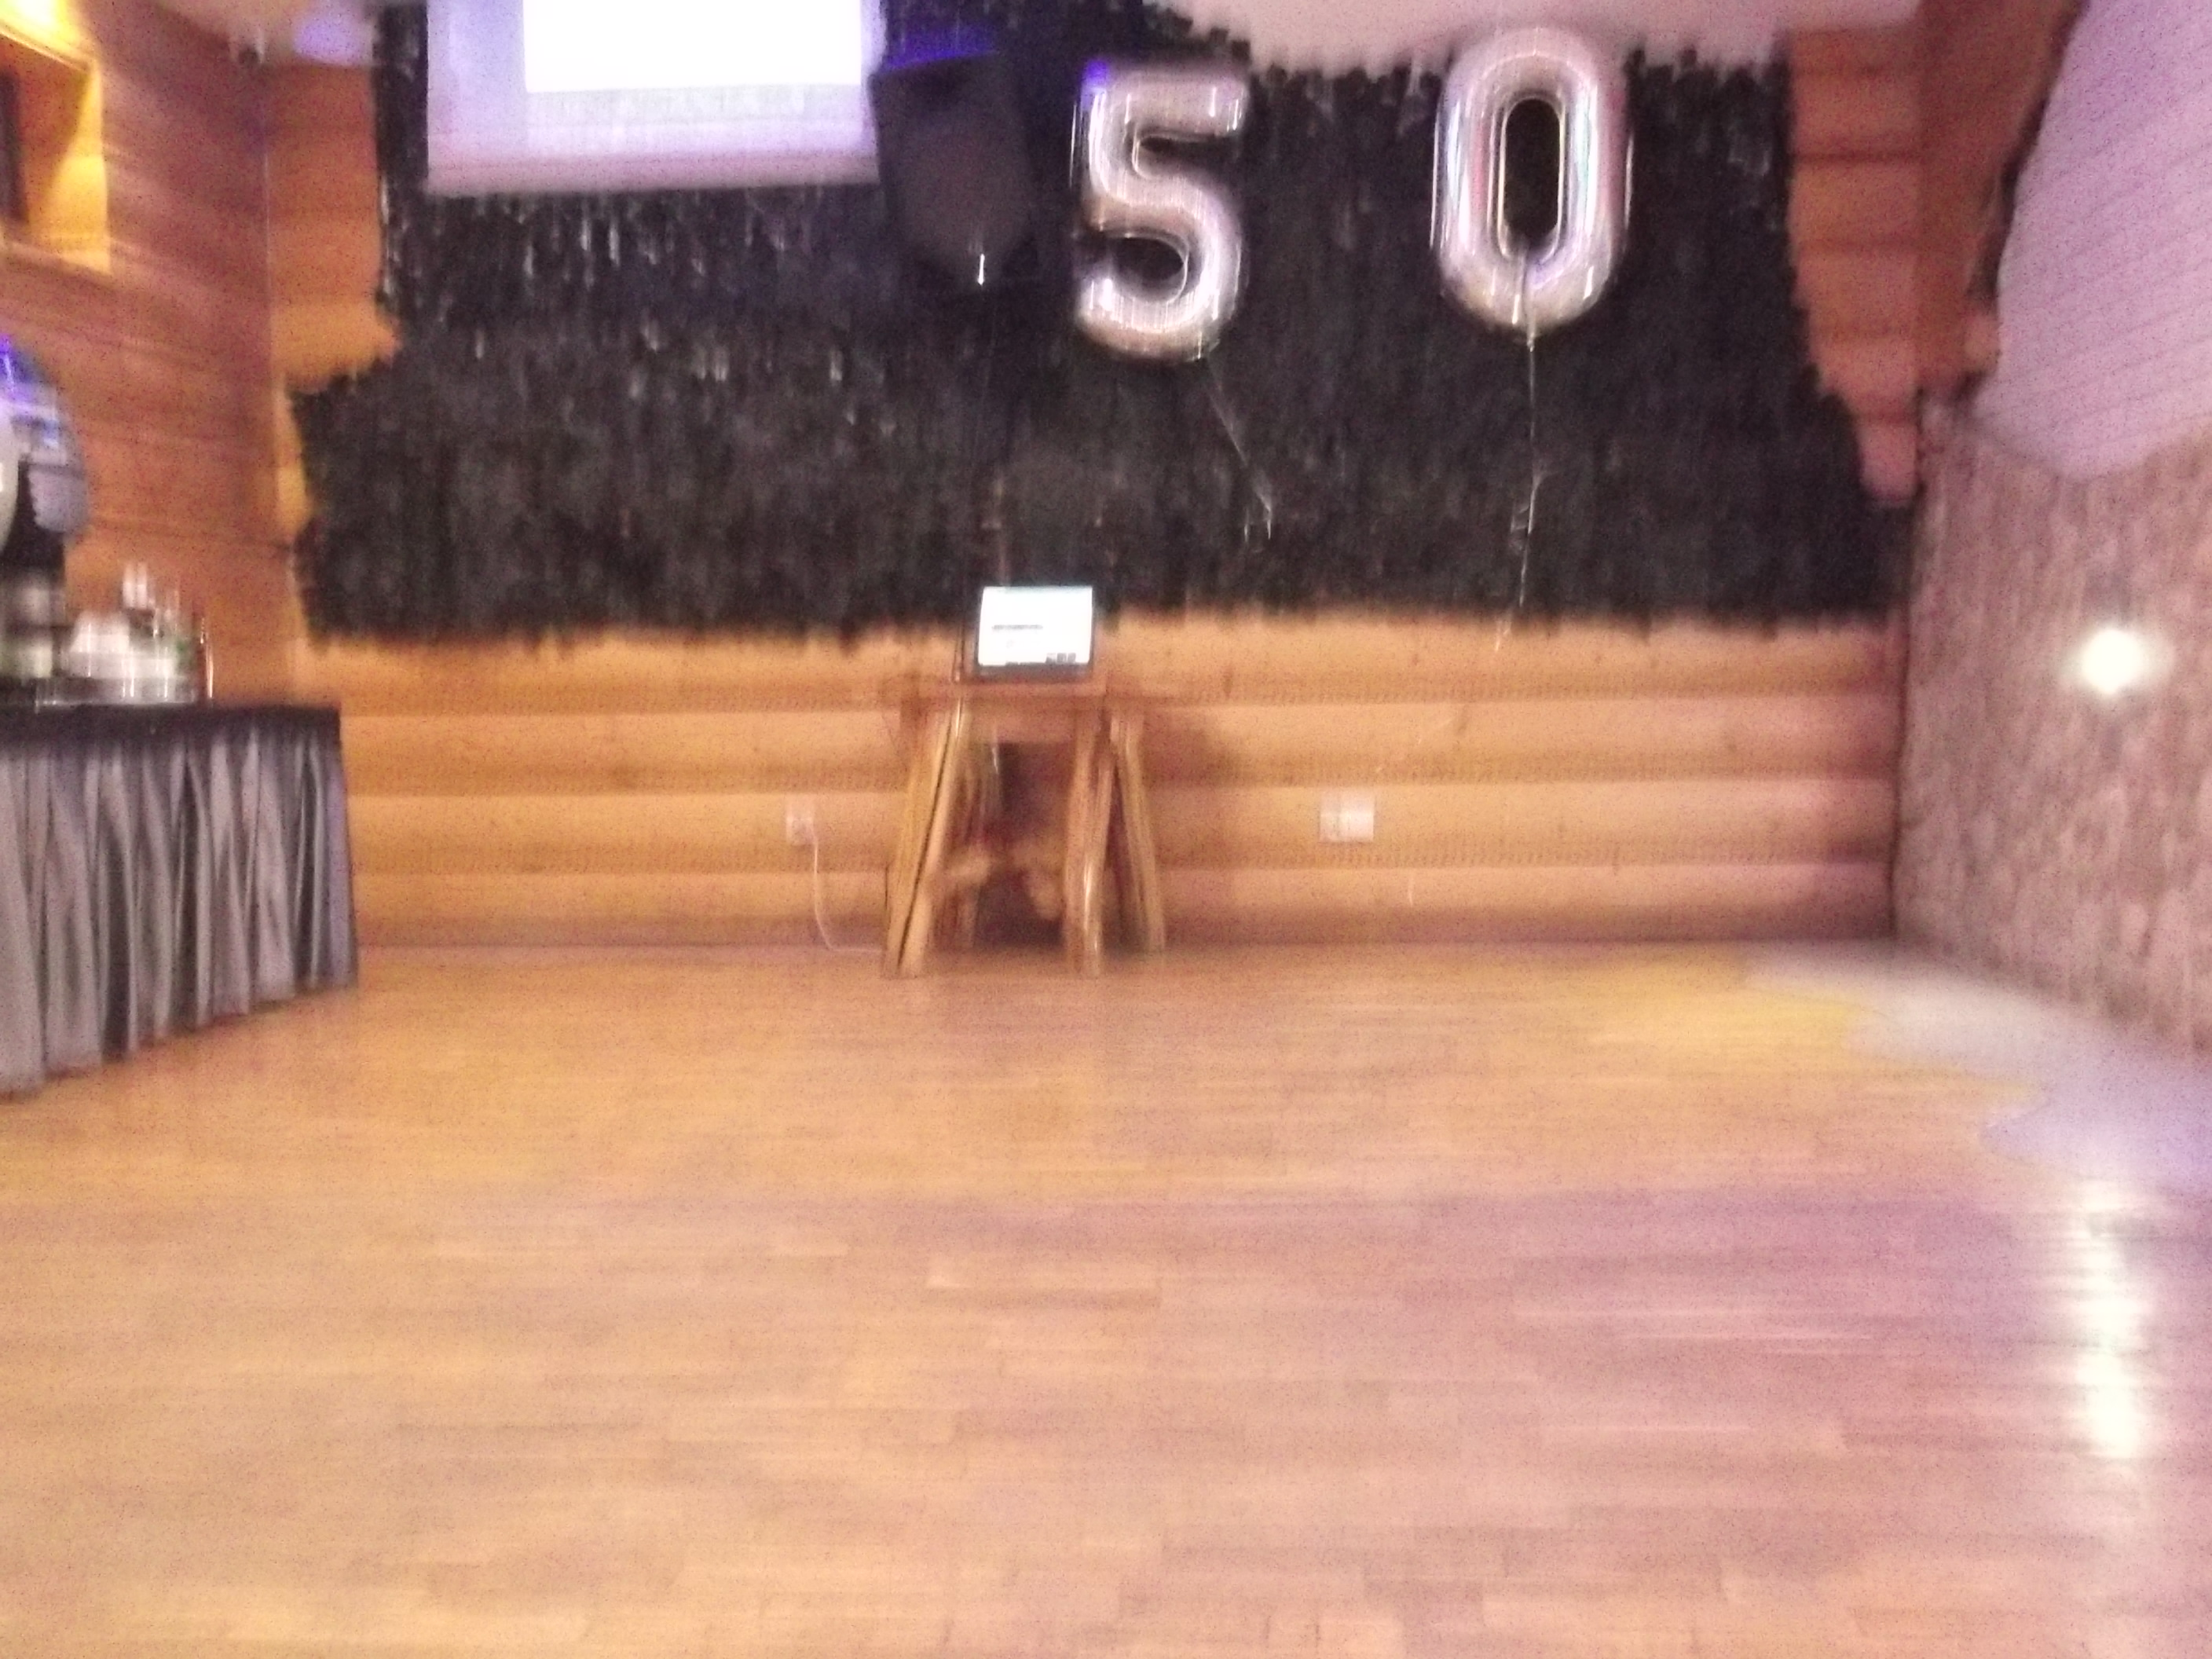
\includegraphics[width=\linewidth, keepaspectratio]{Photos1/photos/balony2.jpg}
    \caption{Zdjęcie doświetlone}
\end{figure}
\begin{figure}[H]
    \centering
    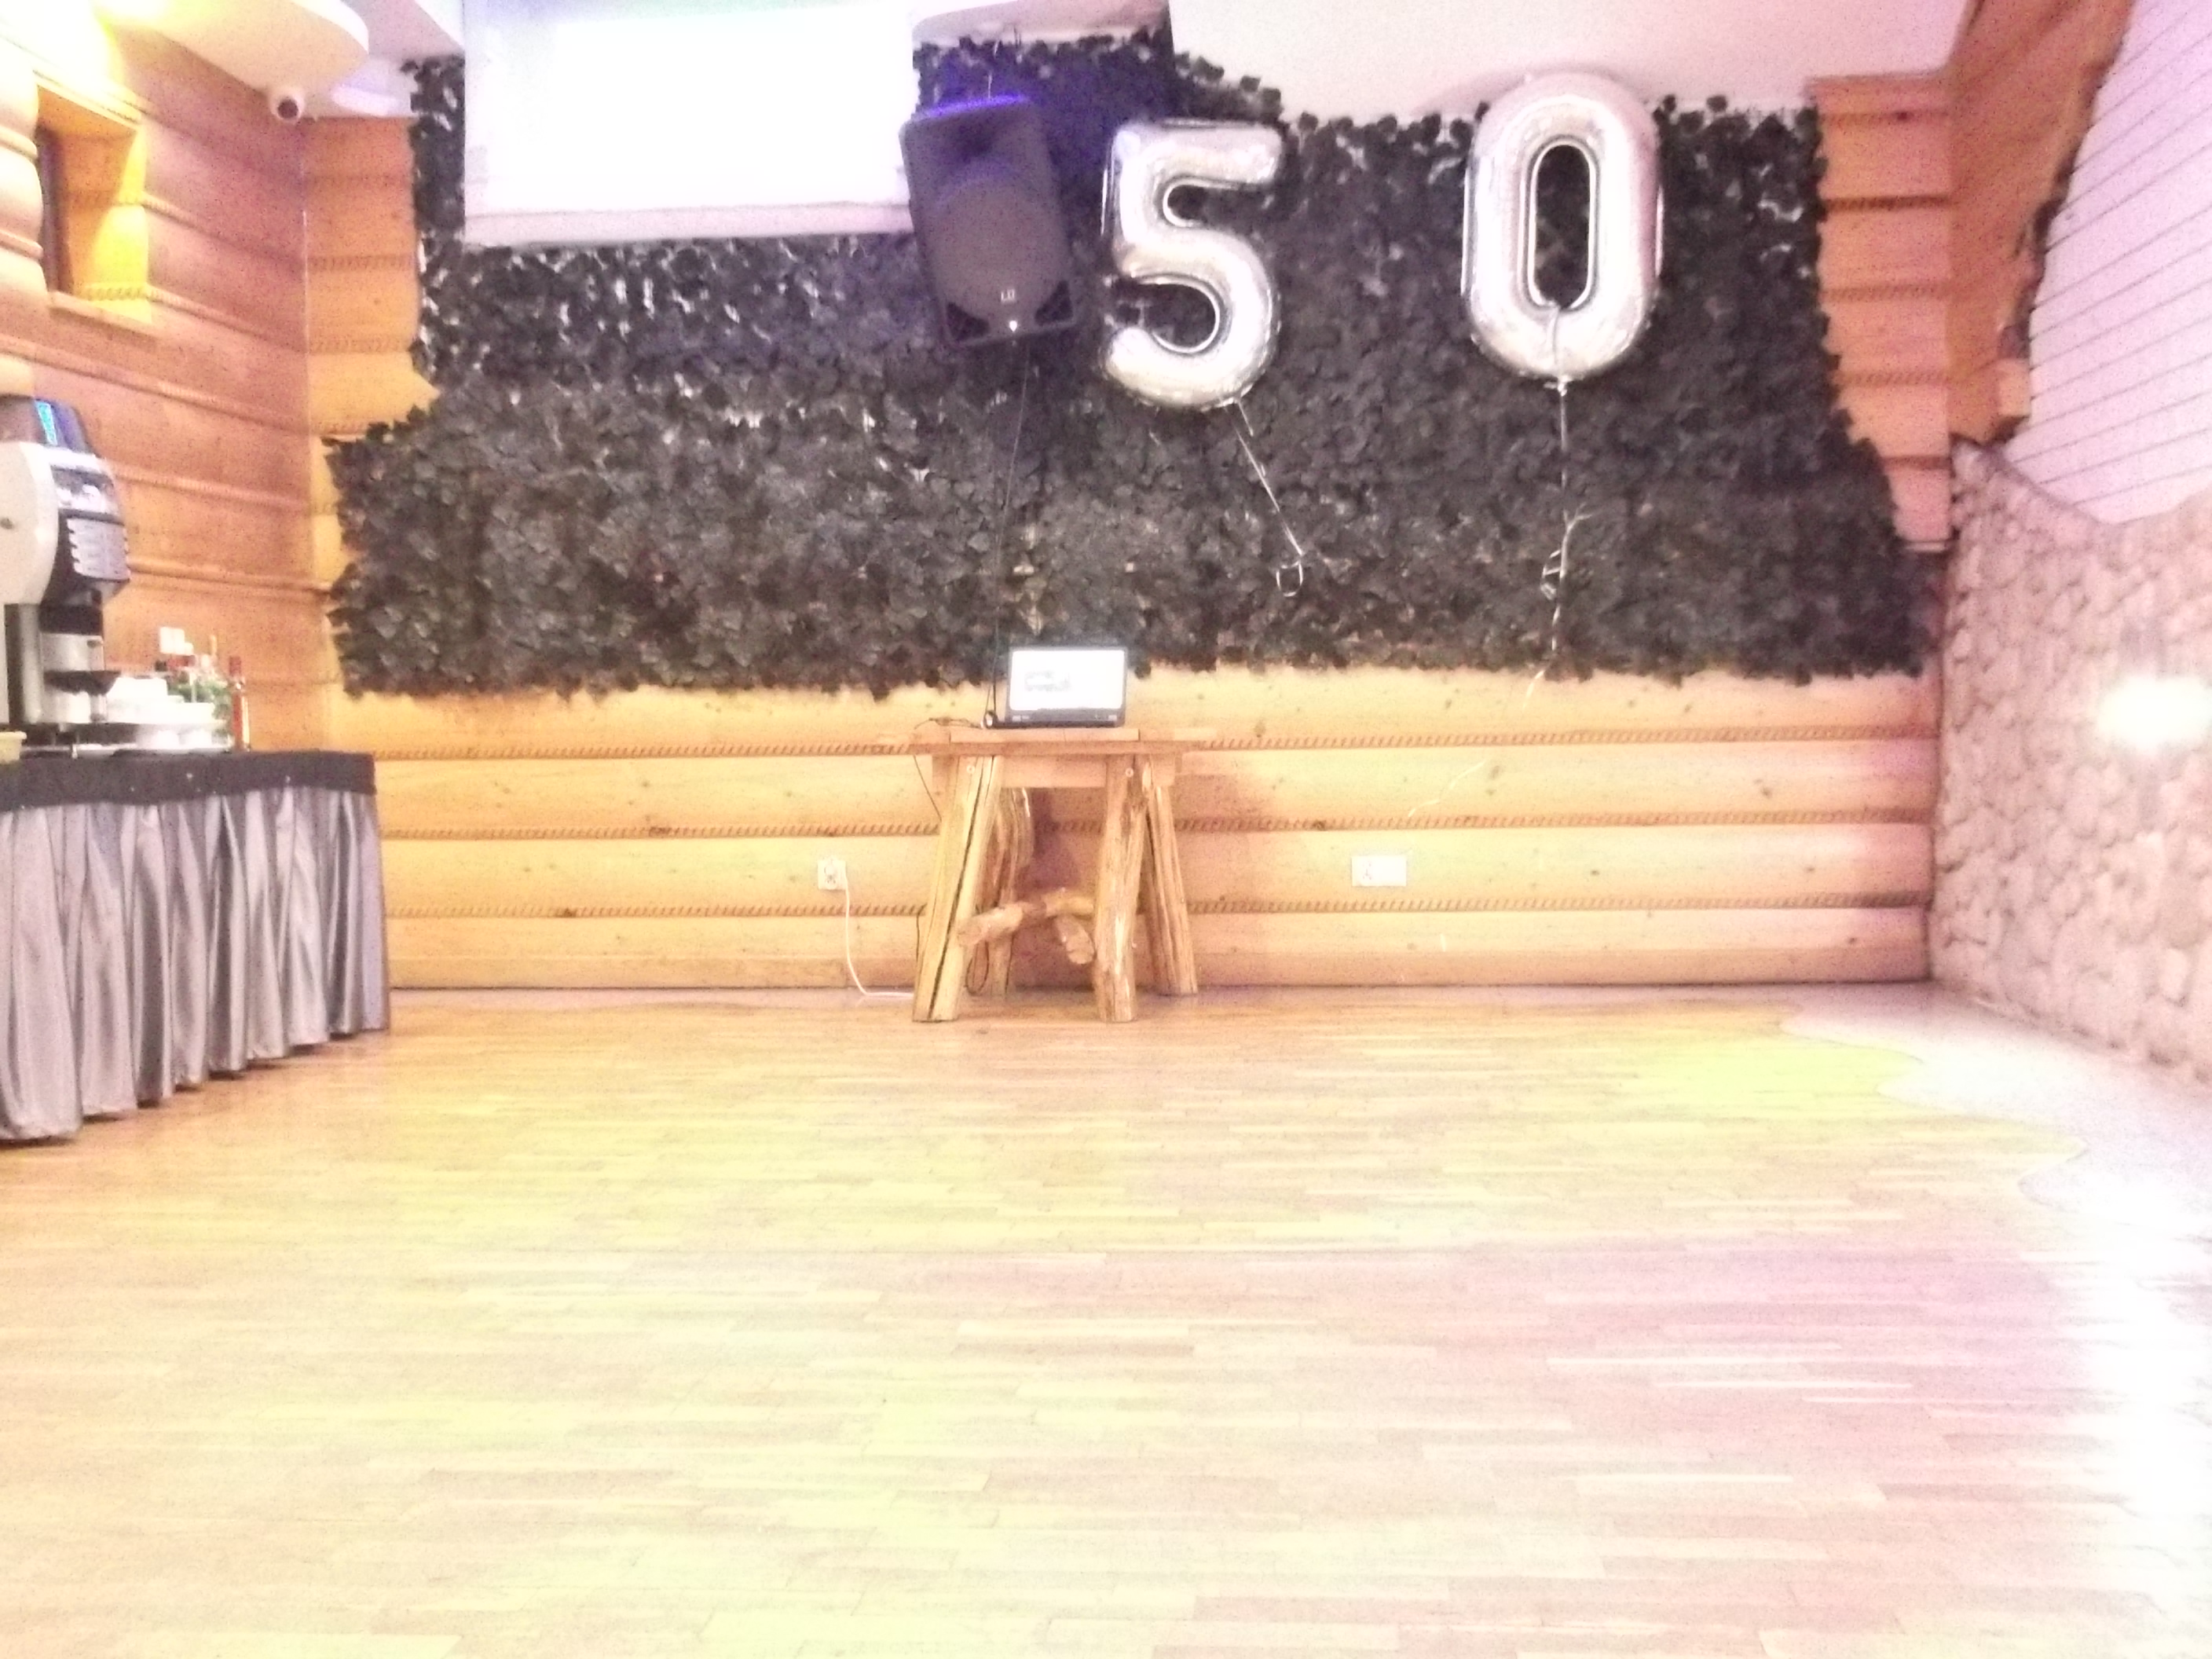
\includegraphics[width=\linewidth, keepaspectratio]{Photos1/photos/balony1.jpg}
    \caption{Zdjęcie prześwietlone}
\end{figure}


\begin{figure}[H]
    \centering
    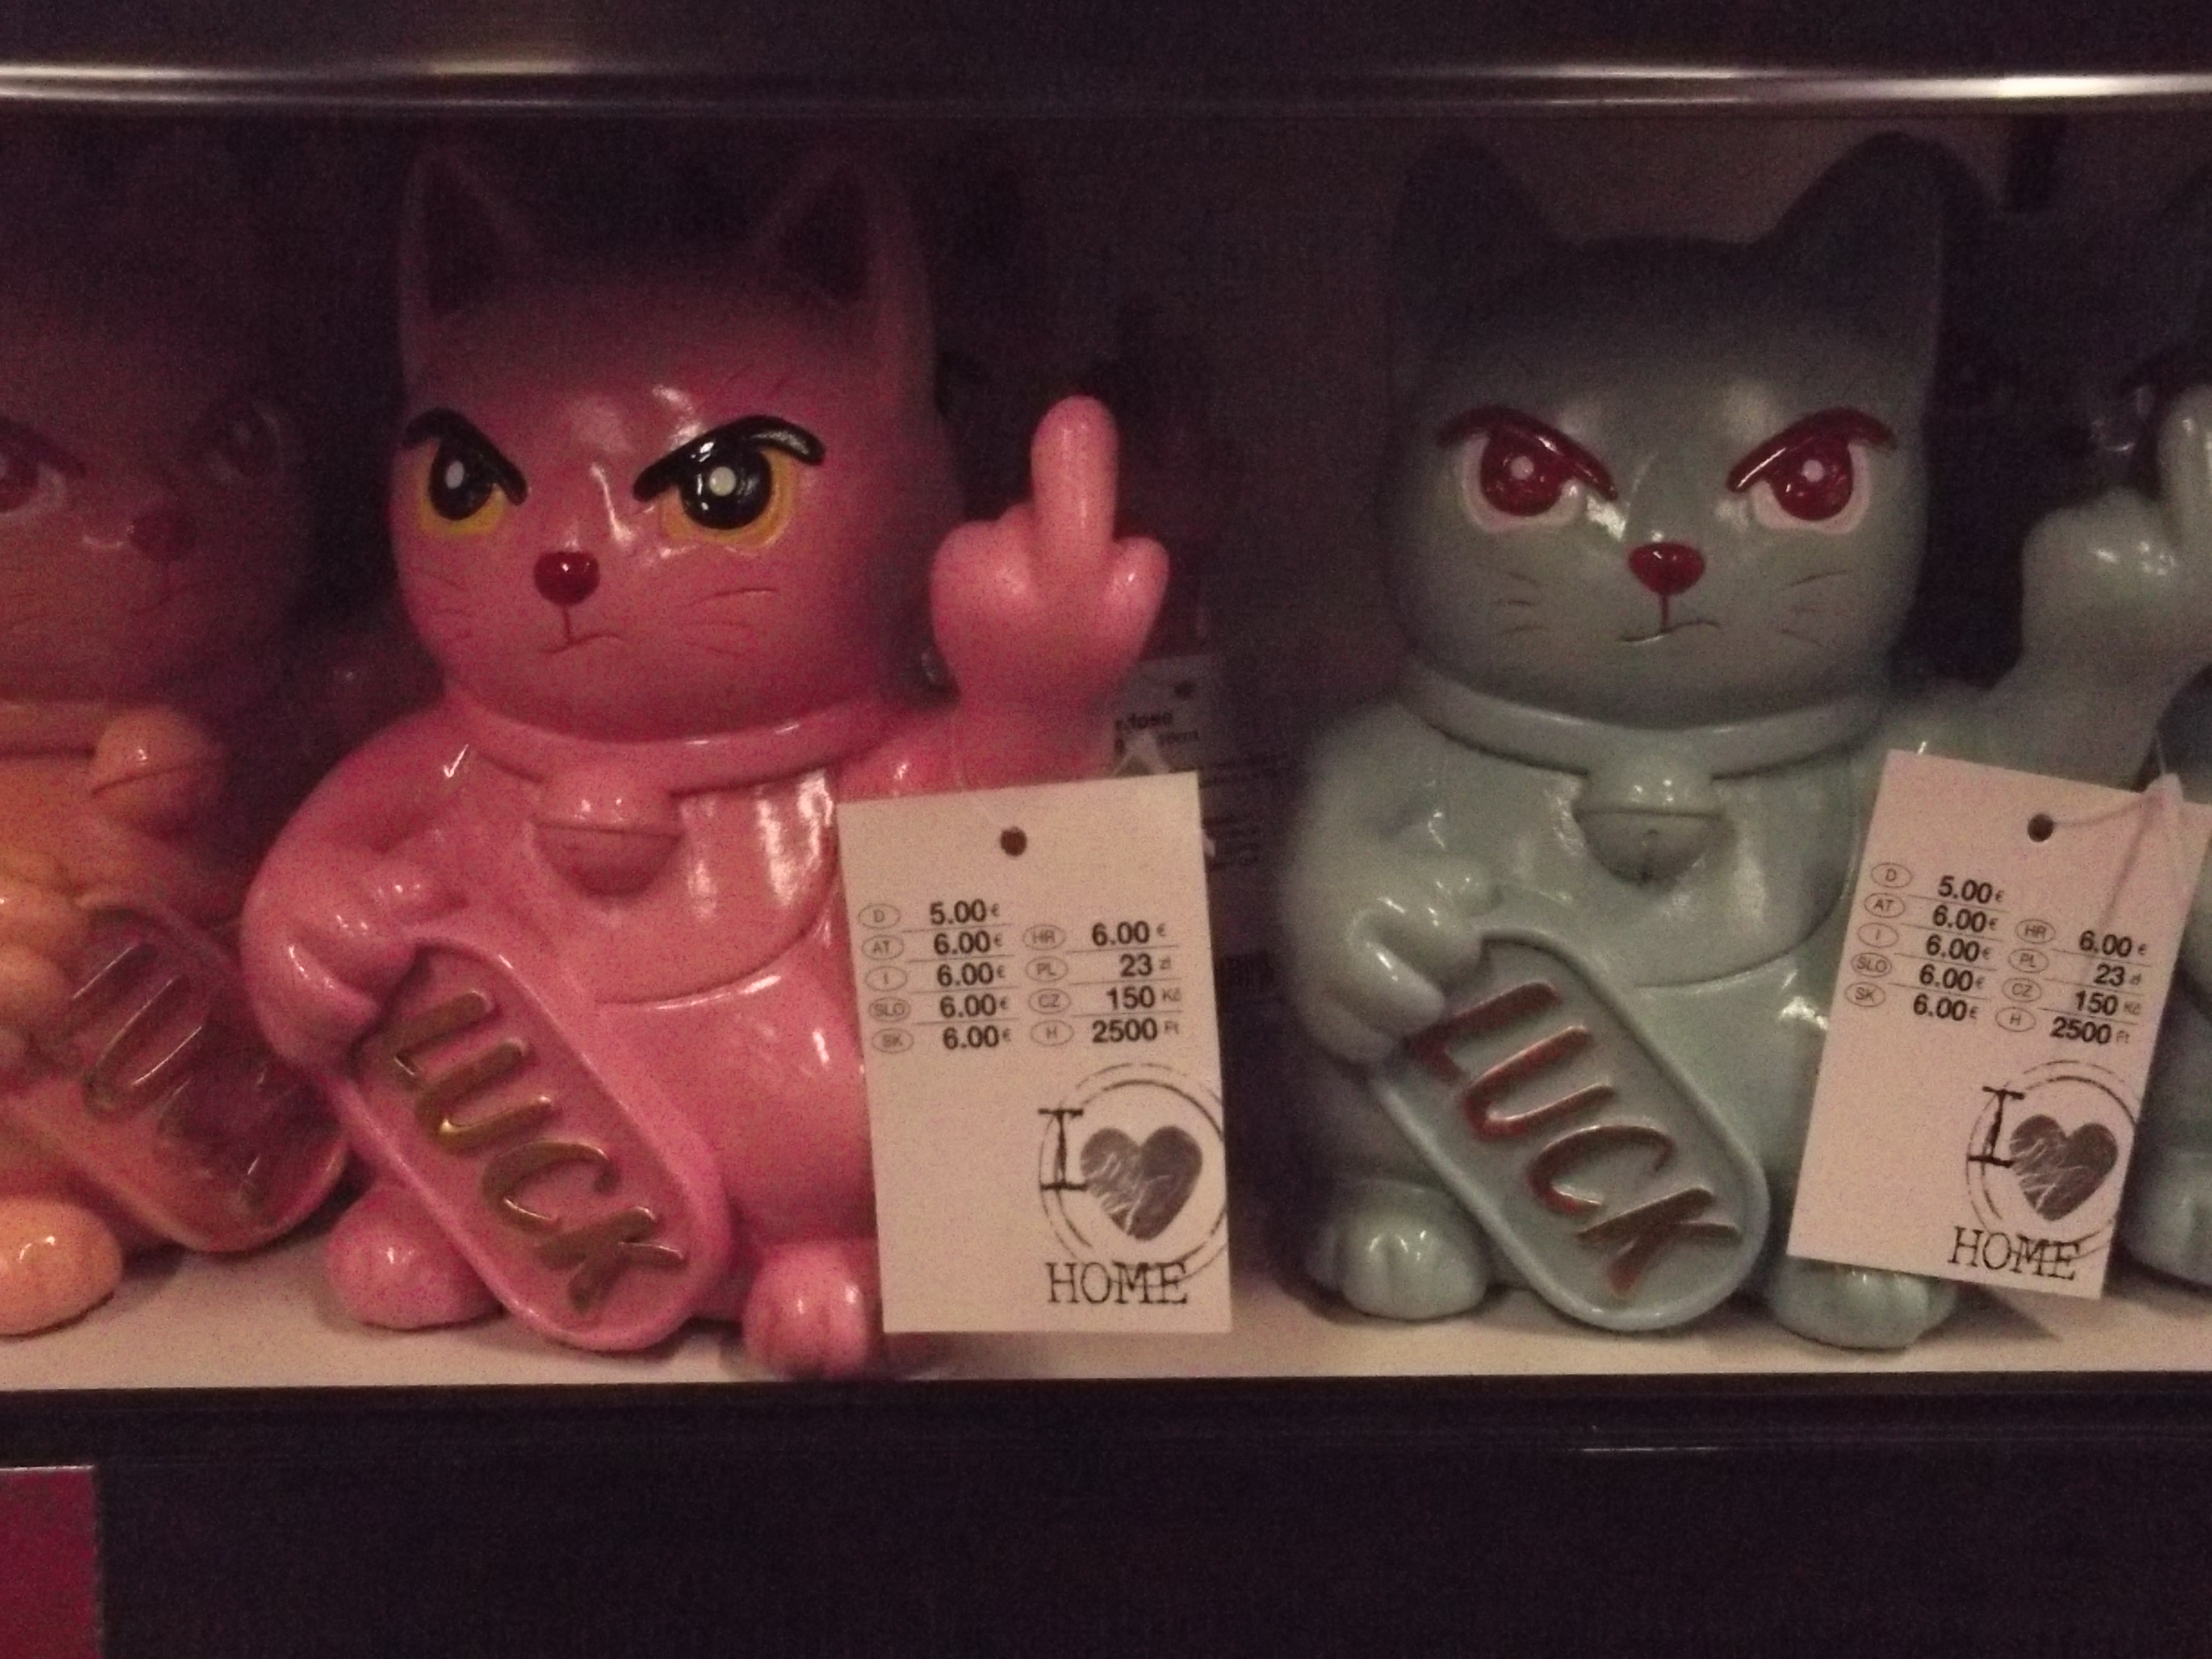
\includegraphics[width=\linewidth, keepaspectratio]{Photos1/photos/kot3.jpg}
    \caption{Zdjęcie niedoświetlone}
\end{figure}
\begin{figure}[H]
    \centering
    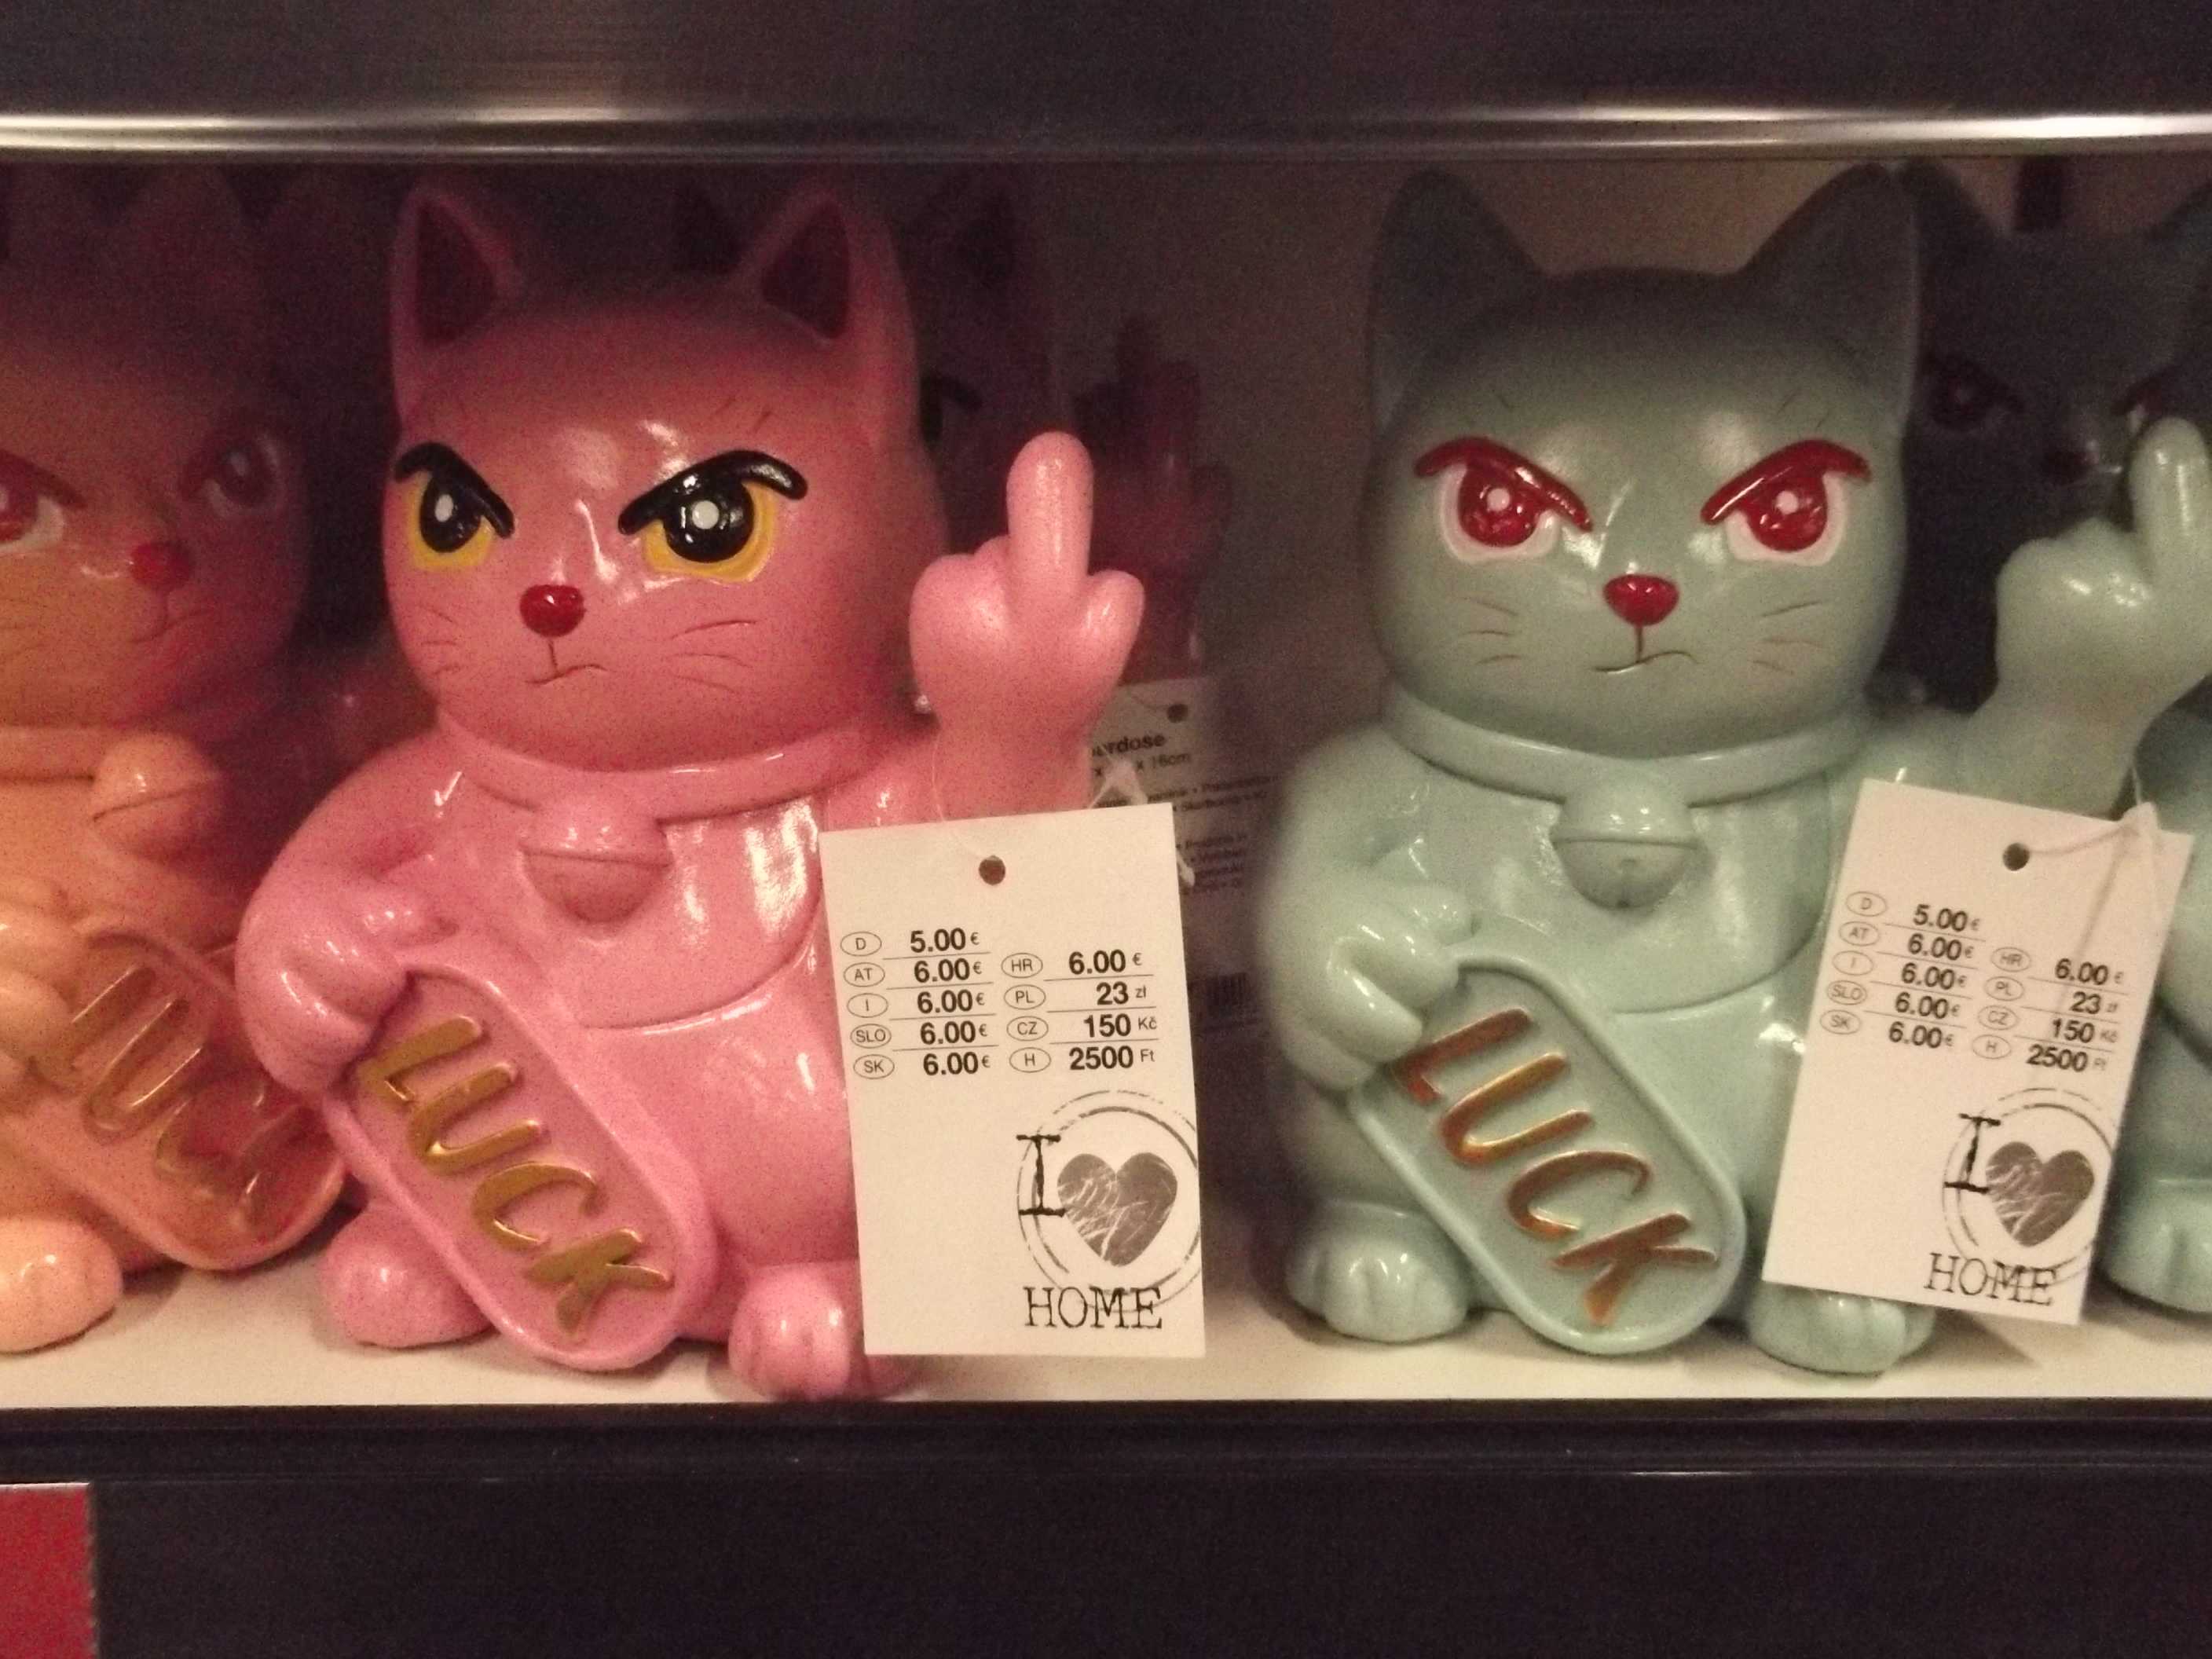
\includegraphics[width=\linewidth, keepaspectratio]{Photos1/photos/kot2.jpg}
    \caption{Zdjęcie doświetlone}
\end{figure}
\begin{figure}[H]
    \centering
    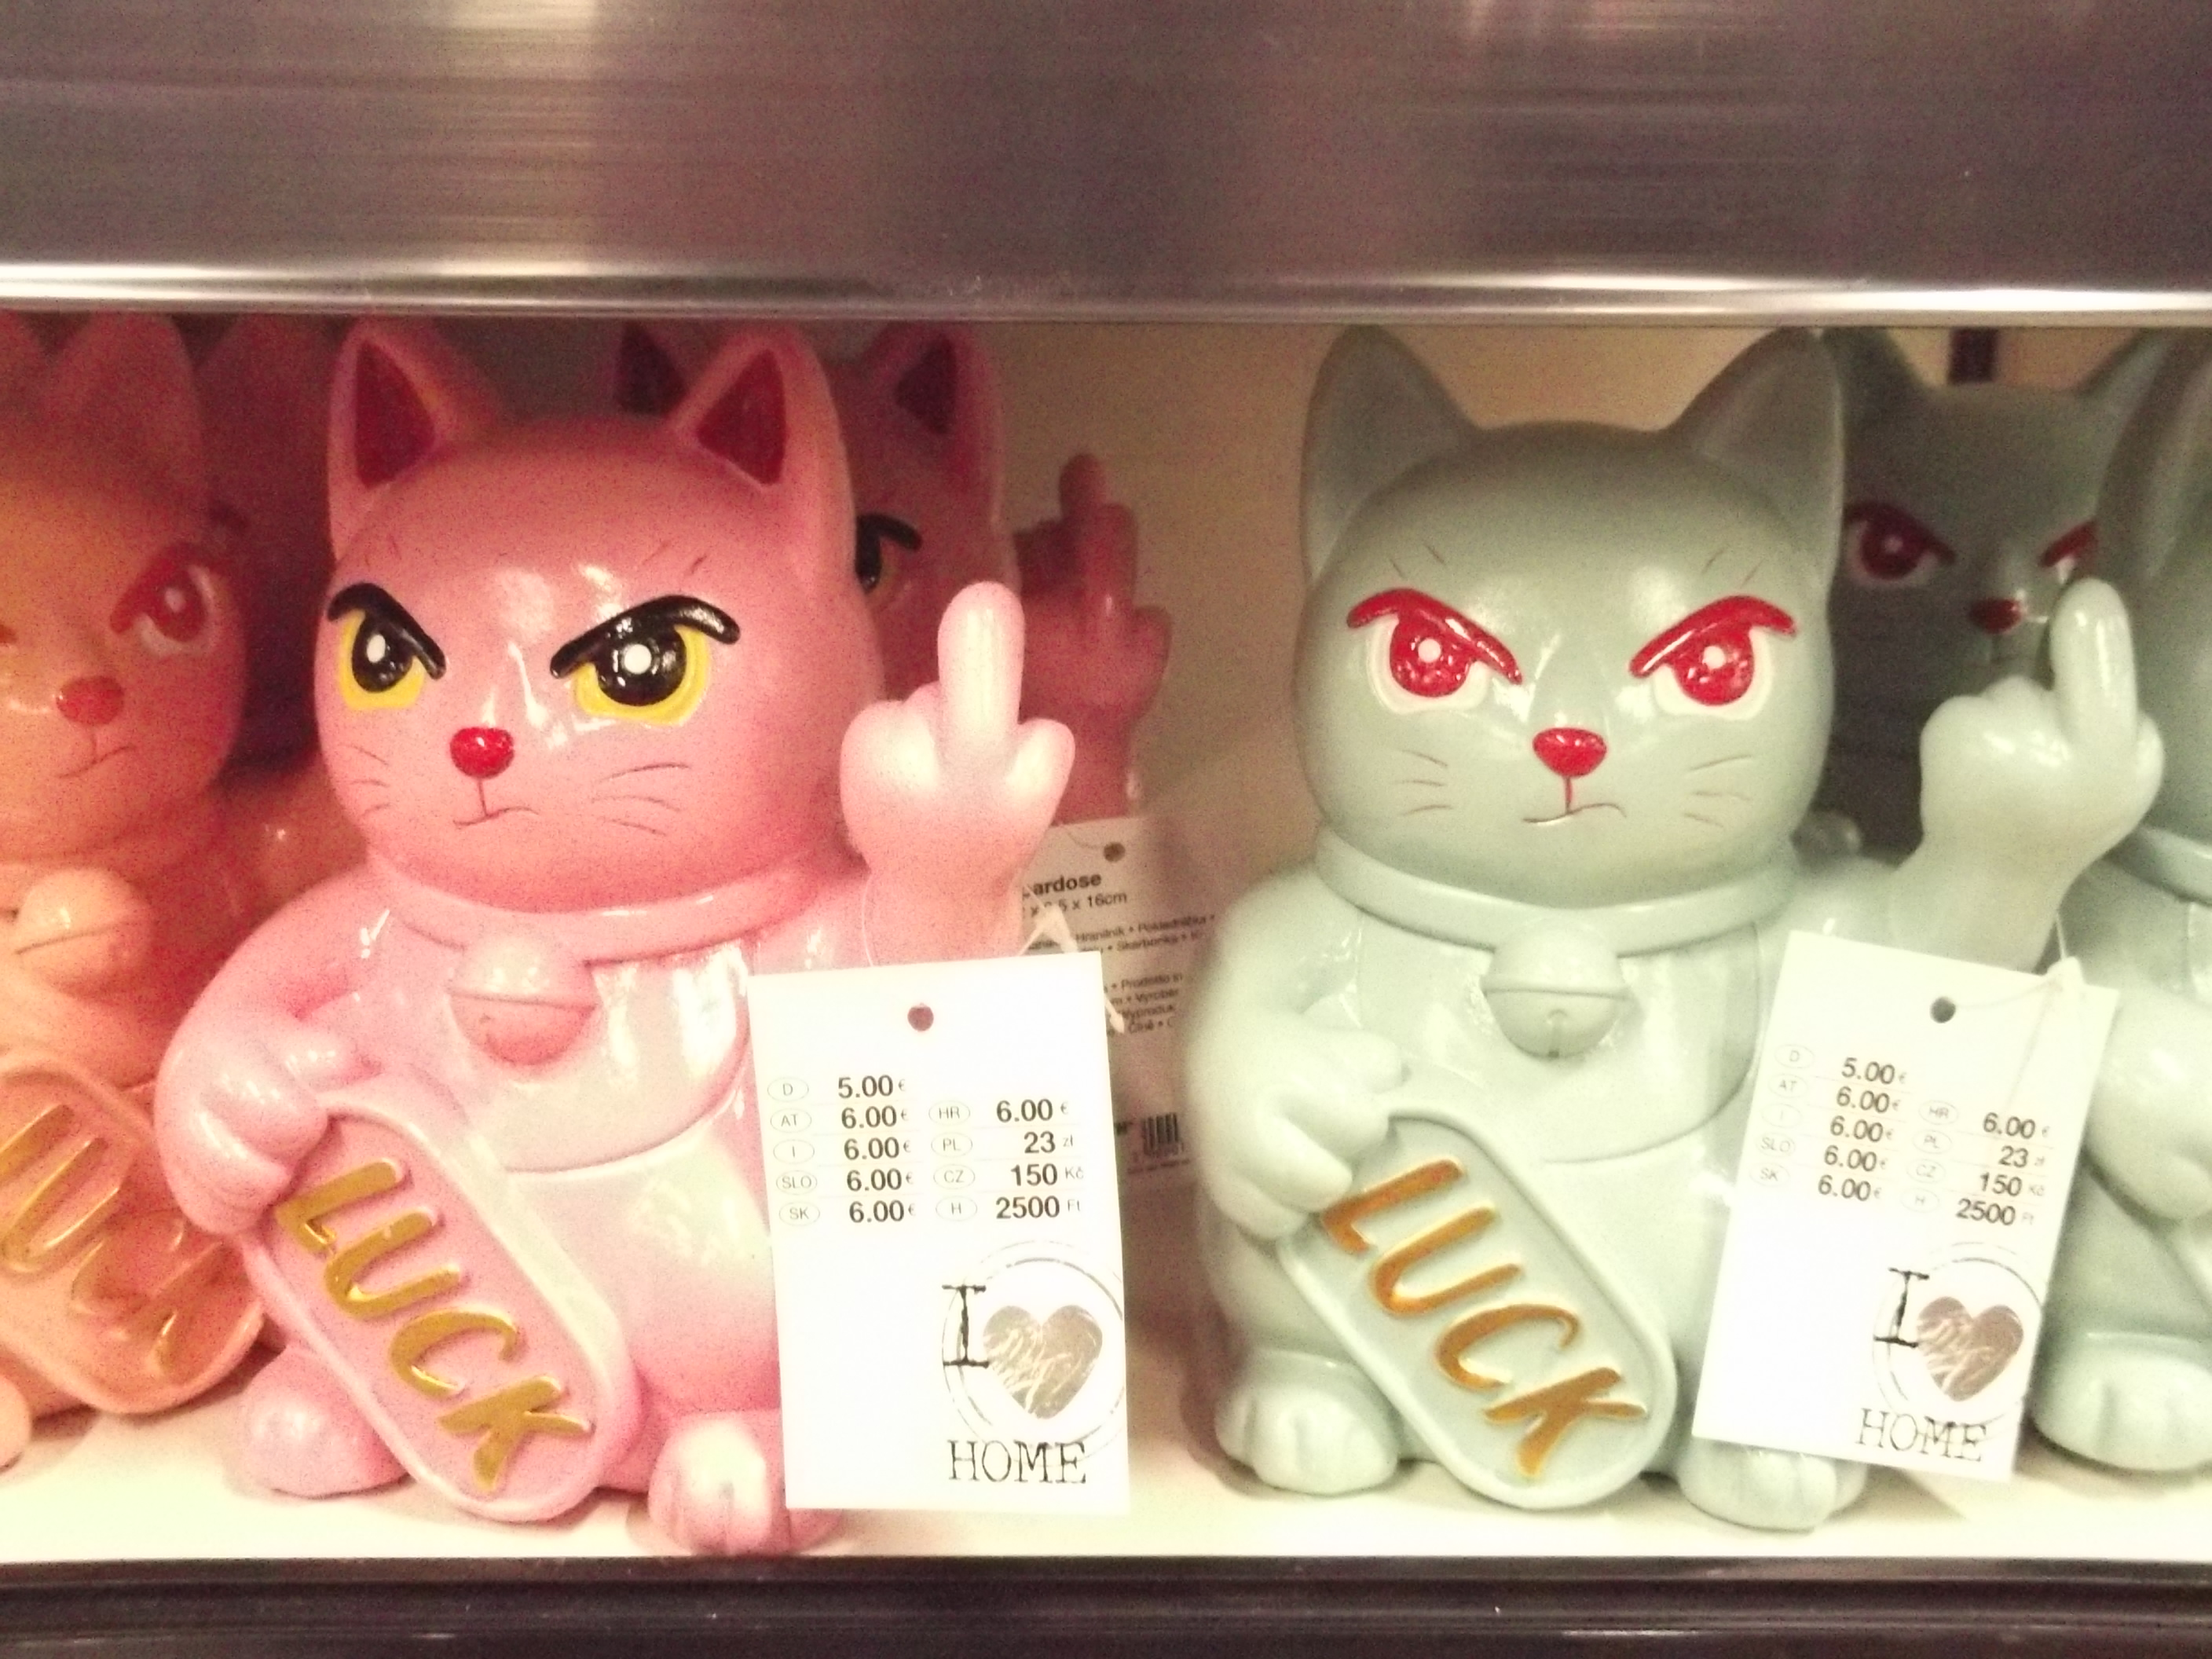
\includegraphics[width=\linewidth, keepaspectratio]{Photos1/photos/kot1.jpg}
    \caption{Zdjęcie prześwietlone}
\end{figure}

\begin{figure}[H]
    \centering
    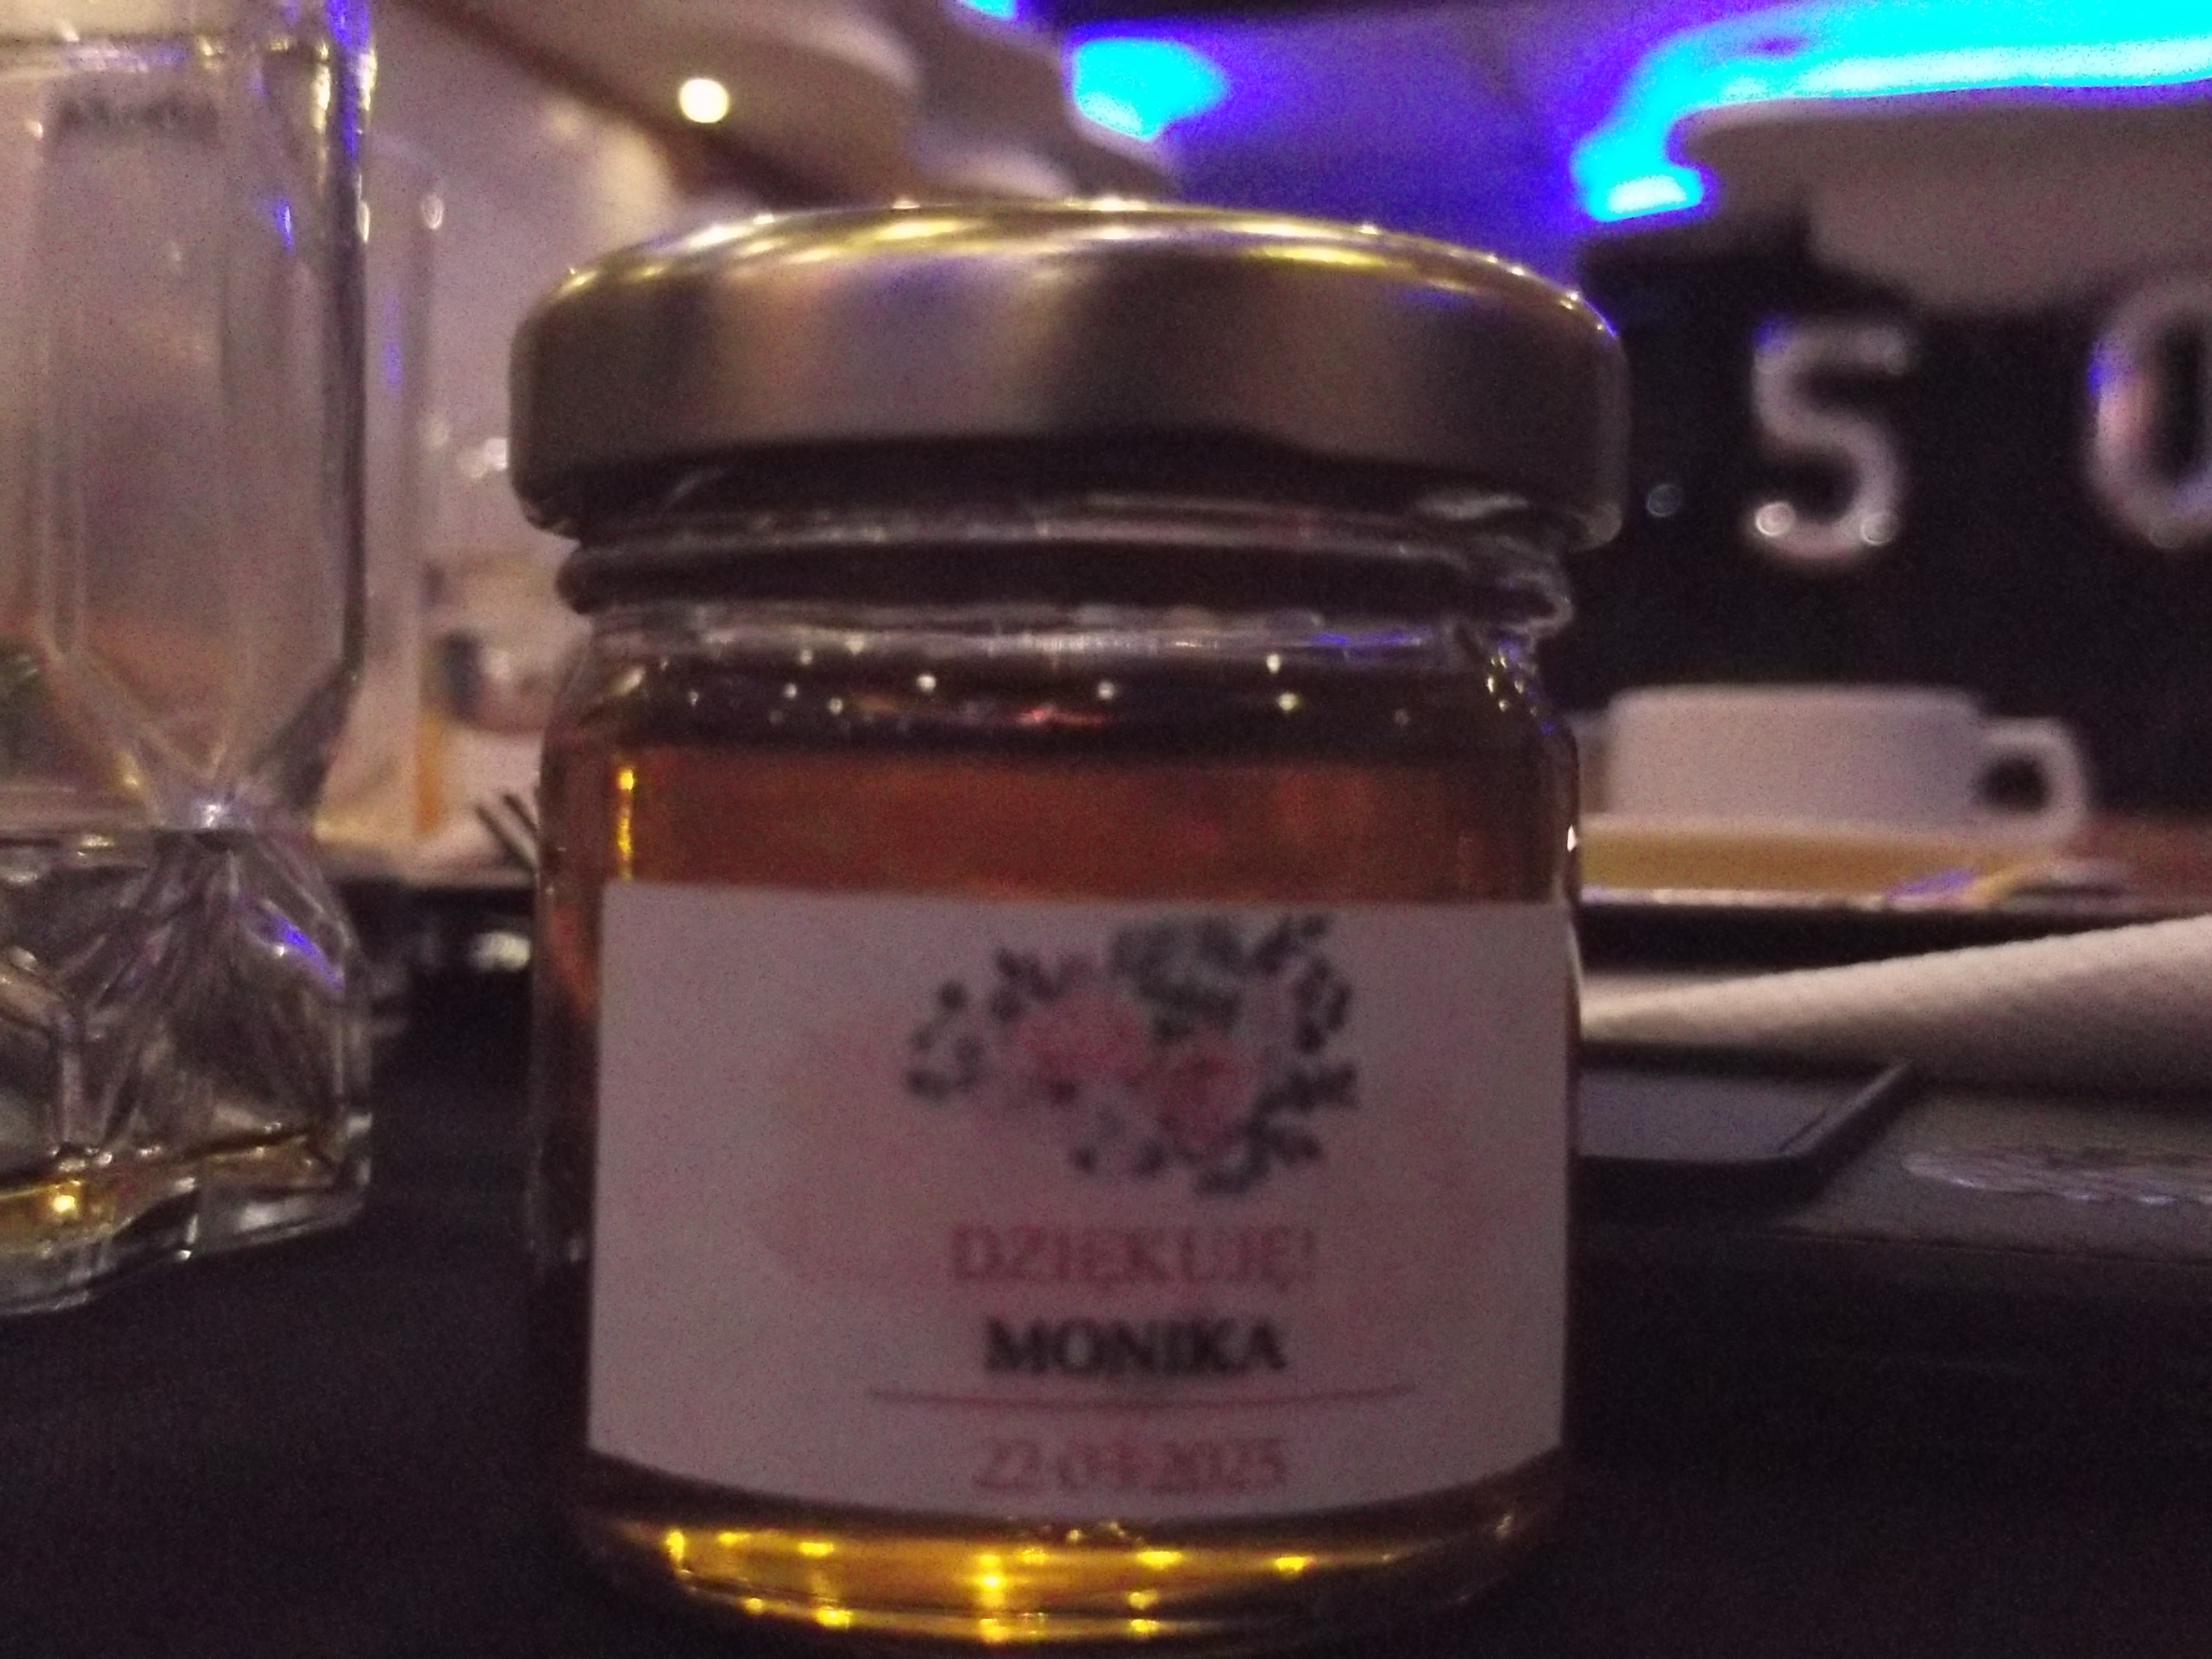
\includegraphics[width=\linewidth, keepaspectratio]{Photos1/photos/miod3.jpg}
    \caption{Zdjęcie niedoświetlone}
\end{figure}
\begin{figure}[H]
    \centering
    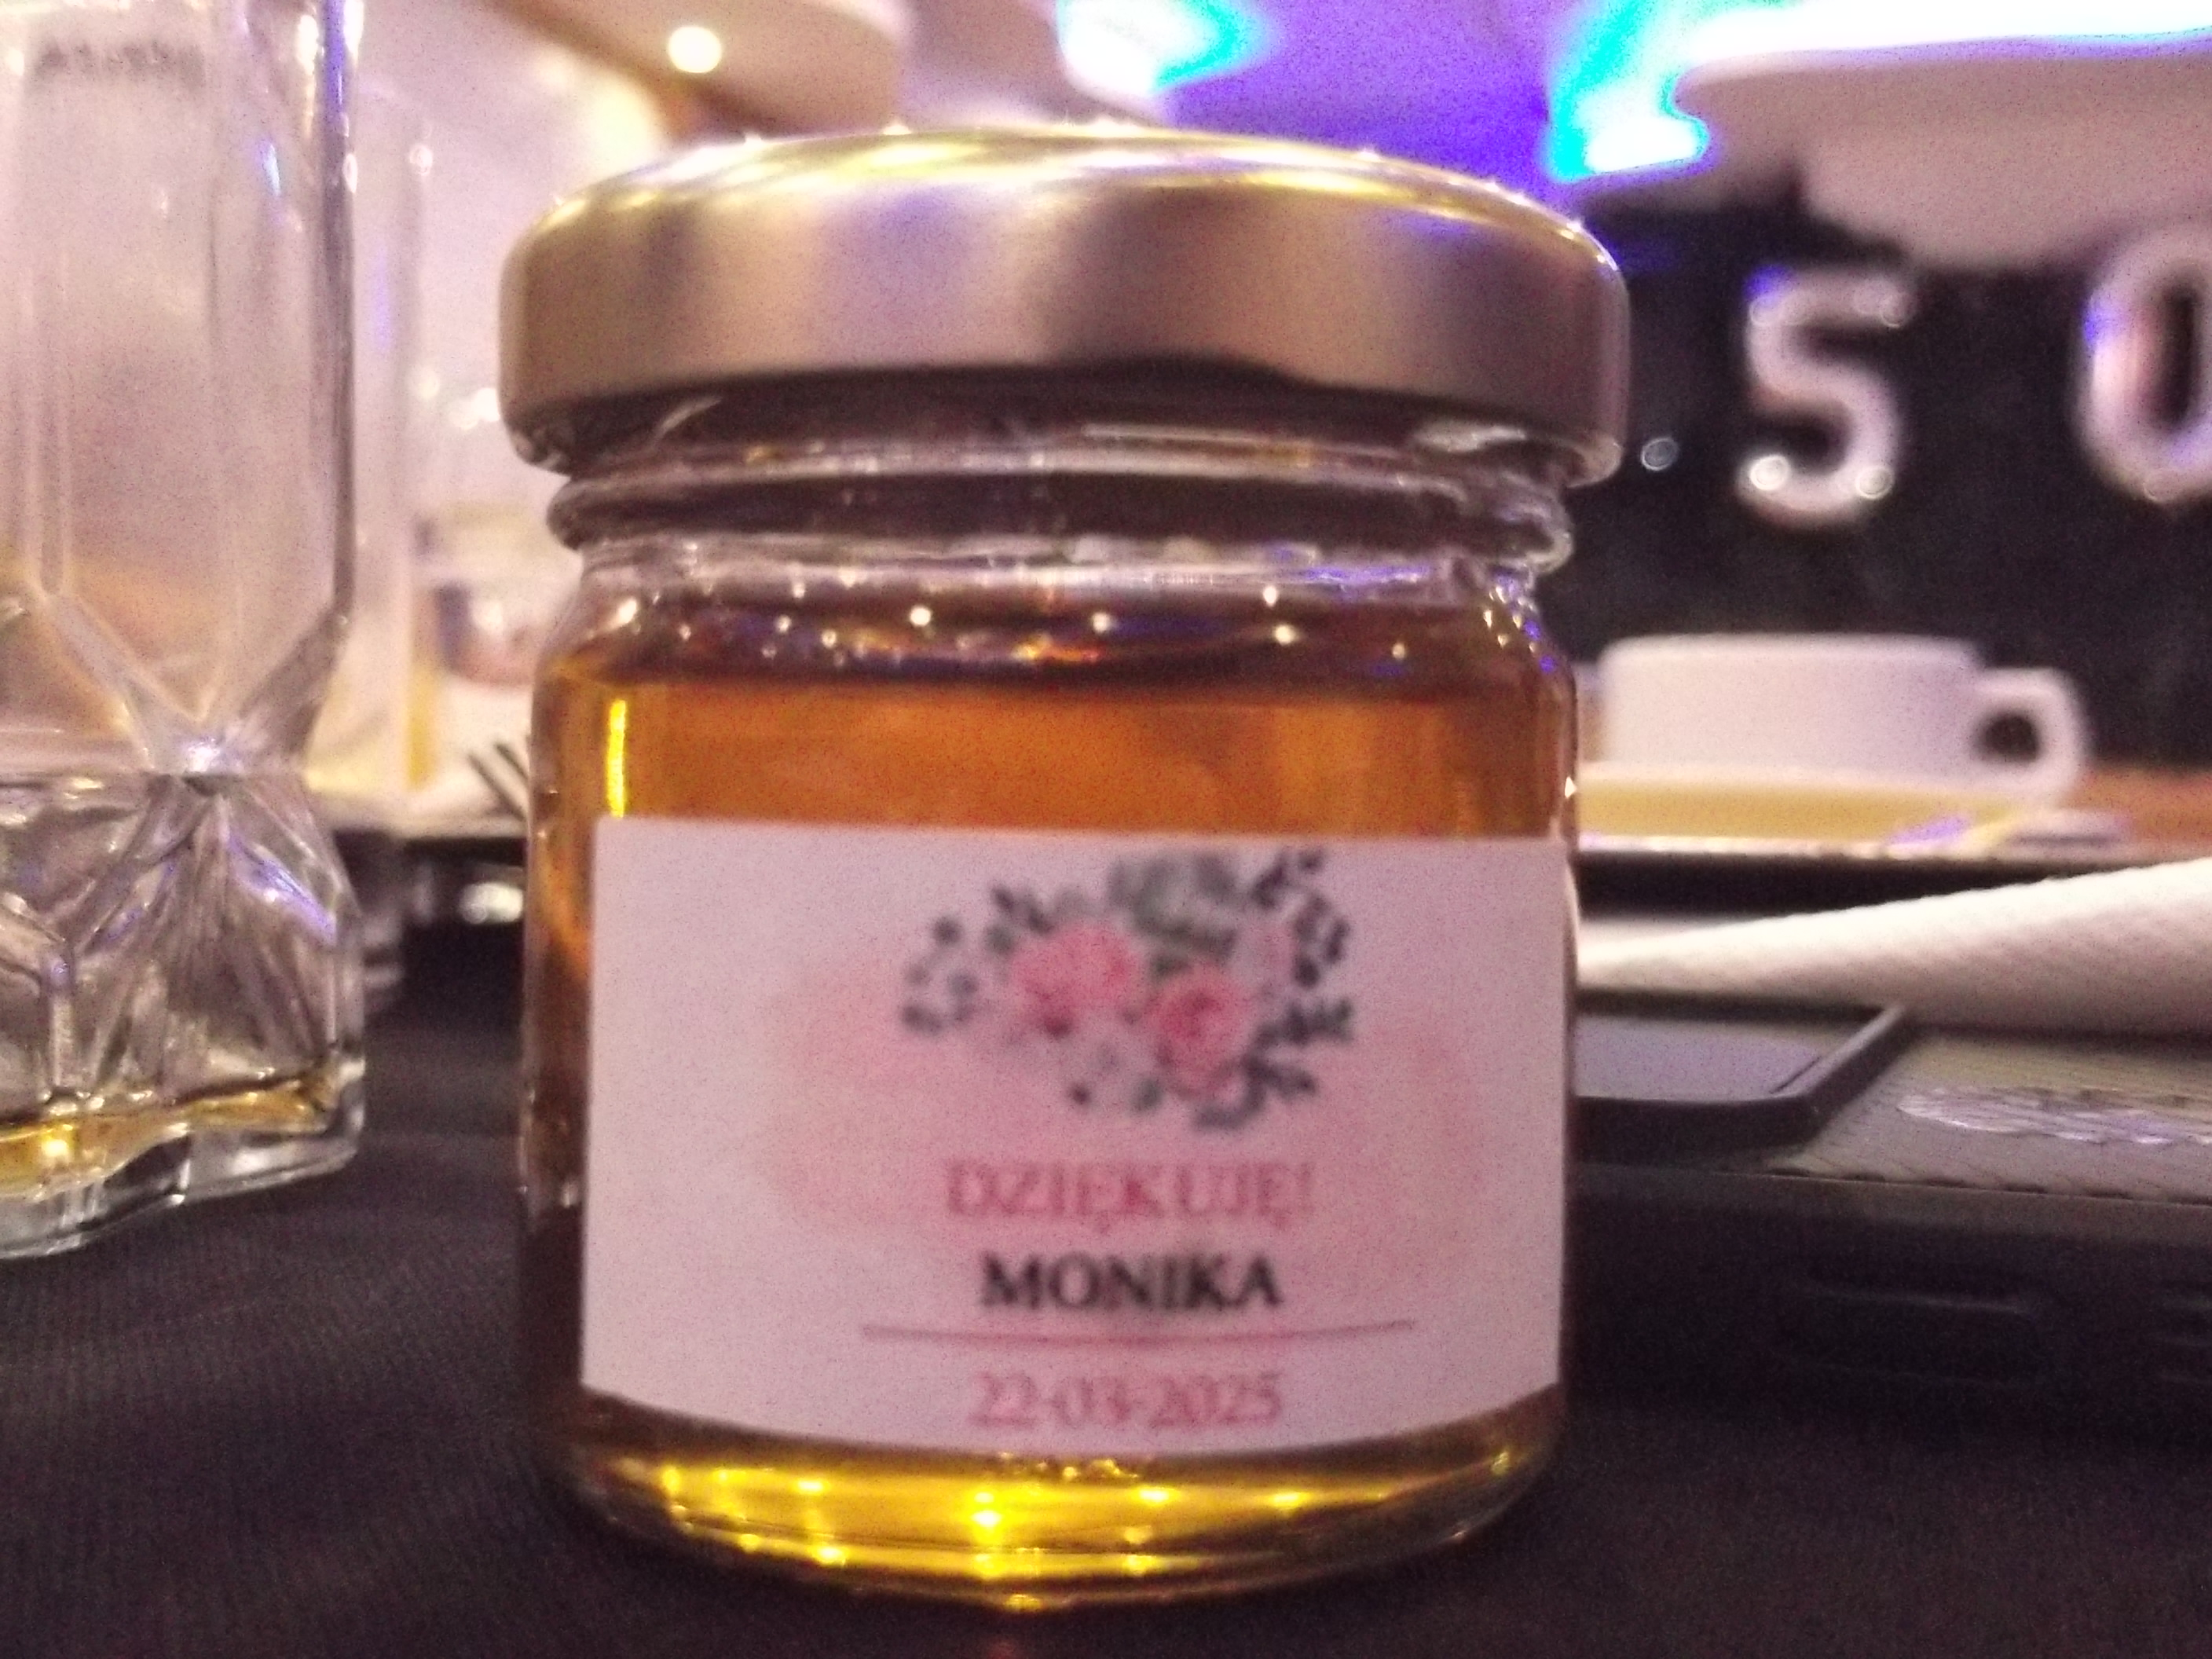
\includegraphics[width=\linewidth, keepaspectratio]{Photos1/photos/miod1.jpg}
    \caption{Zdjęcie doświetlone}
\end{figure}
\begin{figure}[H]
    \centering
    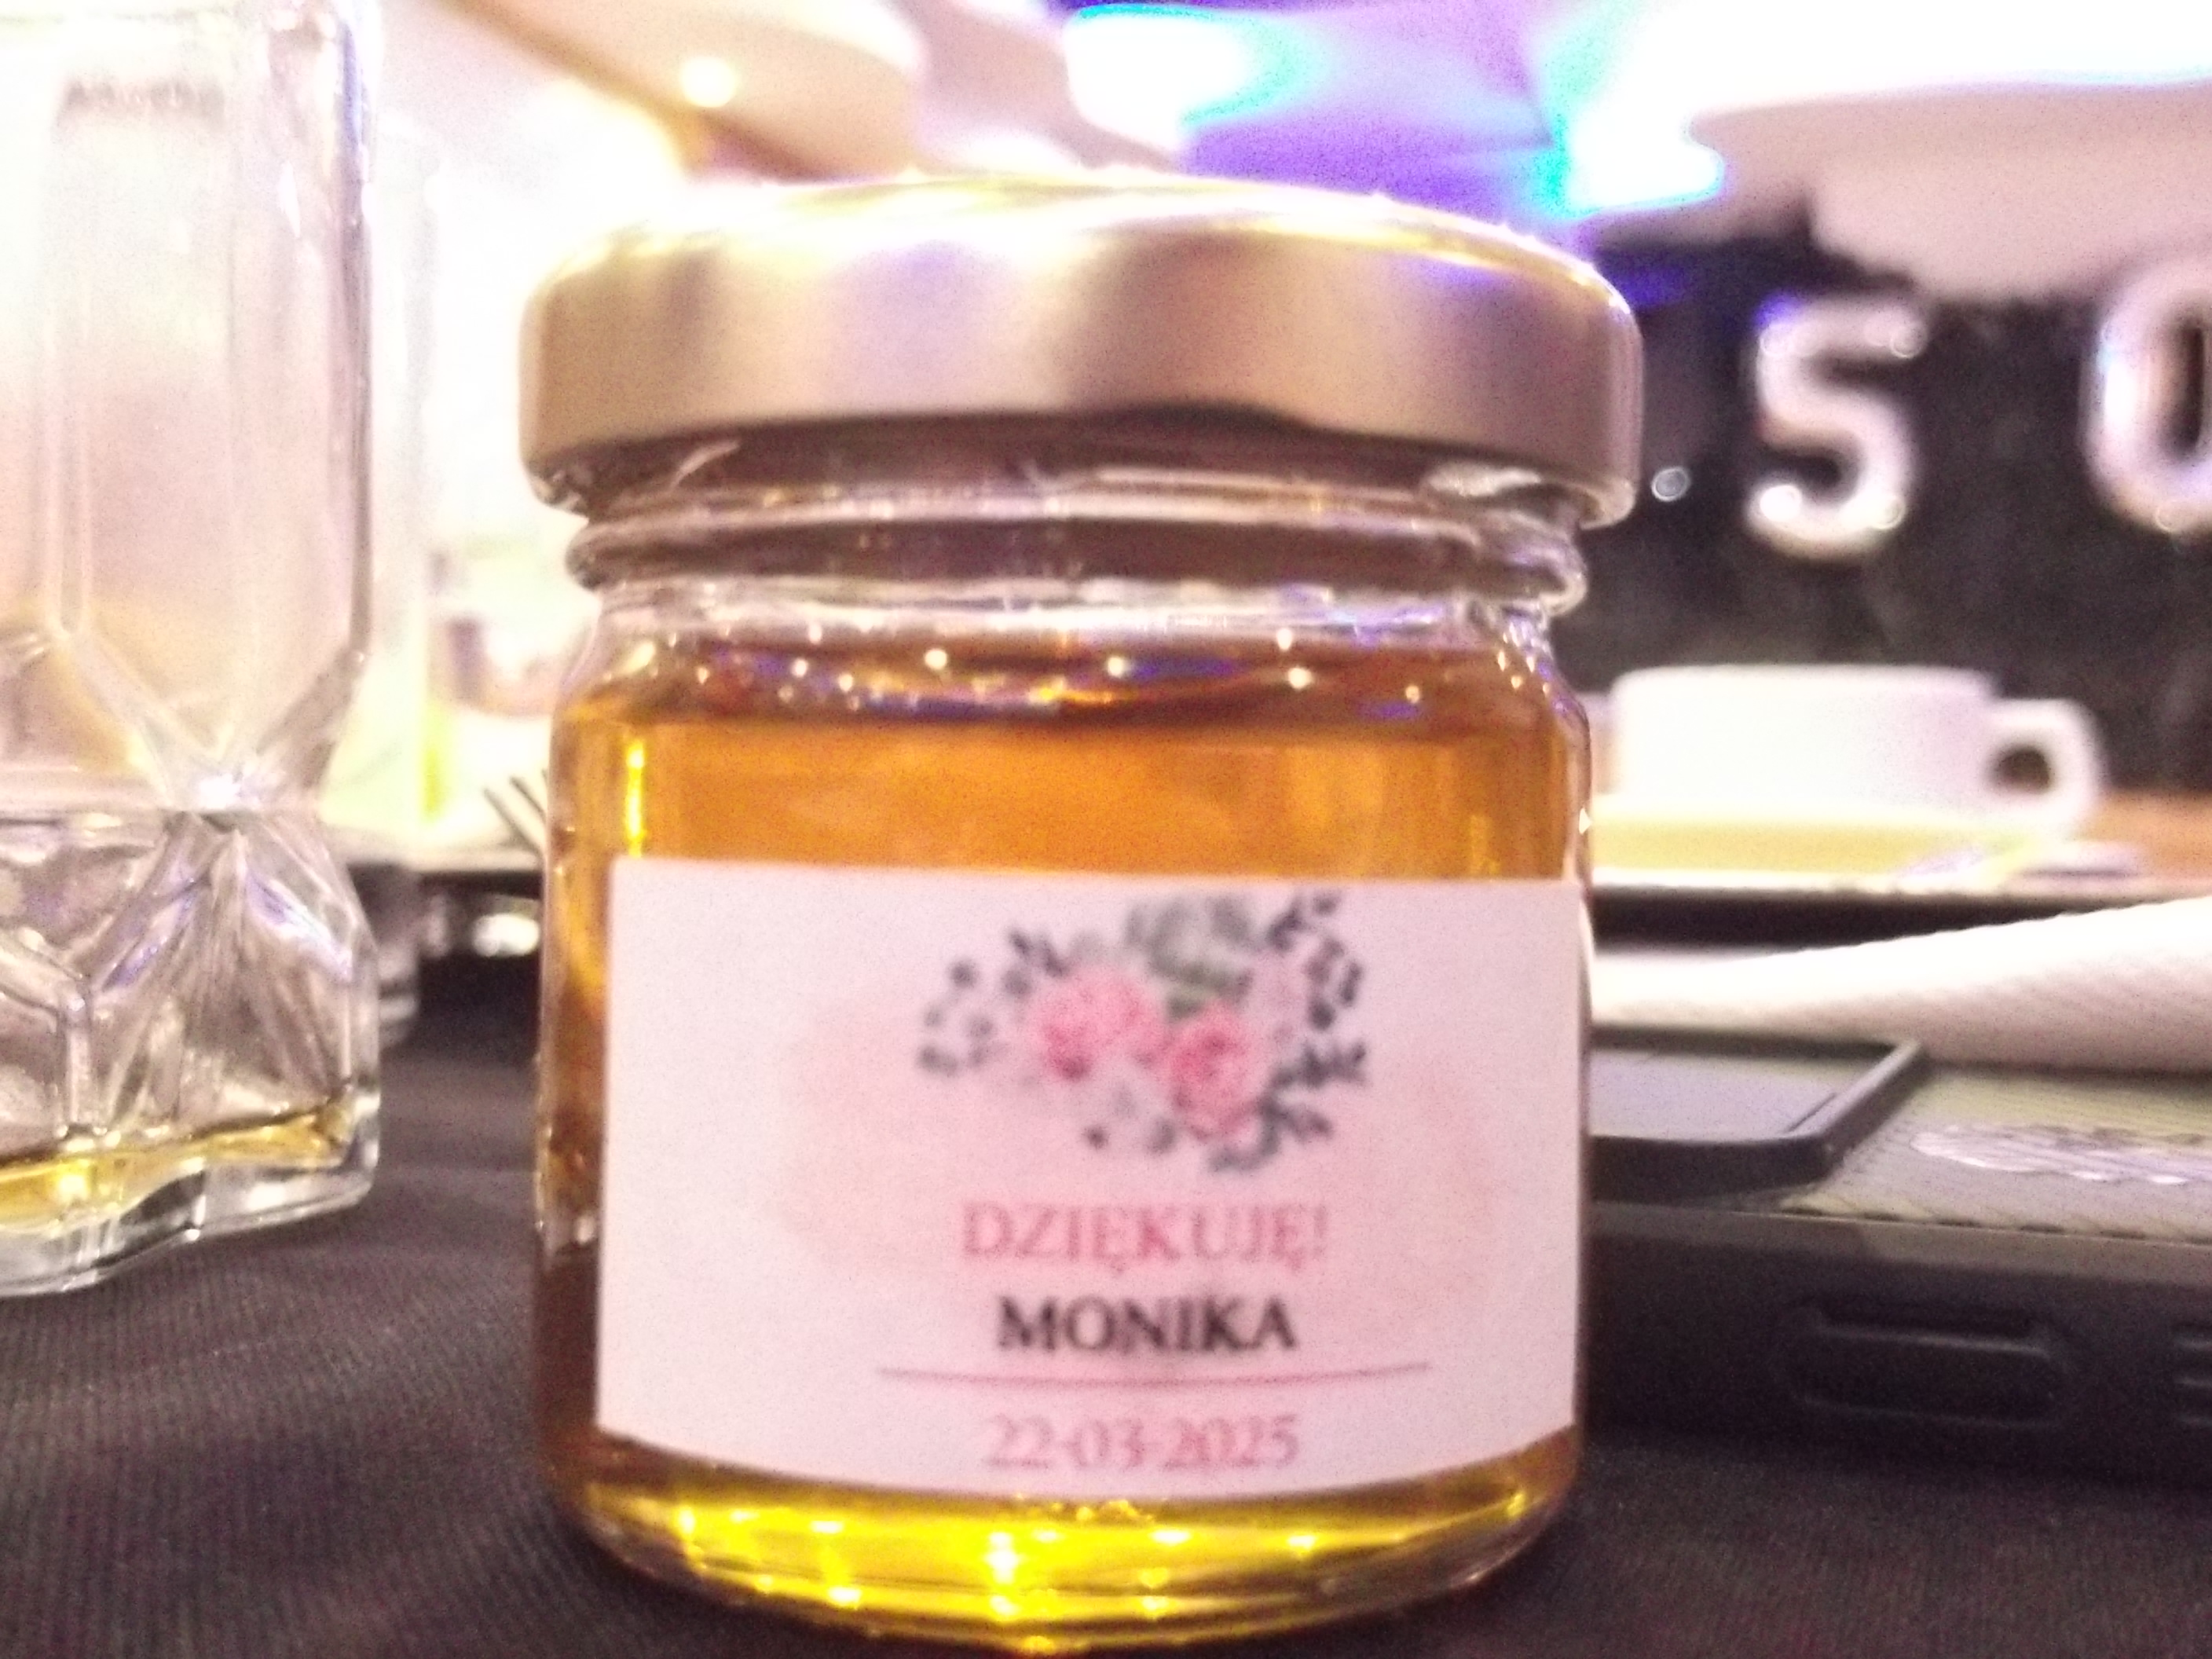
\includegraphics[width=\linewidth, keepaspectratio]{Photos1/photos/miod2.jpg}
    \caption{Zdjęcie prześwietlone}
\end{figure}


Spora (i ciągle rosnąca) baza zdjęć analogowych i cyfrowych dogłębnie ilustrujących
sedno problemu z którym się zmagamy znajduje się tutaj:
\url{https://drive.google.com/drive/folders/1SFu_A46nBXhL19diXnxV-iyEyH0fnhFA}








\section{Wstępna analiza}
Jakkolwiek często `na oko' względnie łatwo porównując dwa zdjęcia wskazać
to, któremu brakuje szczegółów lub zostało niedoświetlone, to warto się
zastanowić co tak właściwie znaczy to, że zdjęcie jest niedoświetlone. \newline

W celu analizy i próby zdefiniowania zdjęcia o skrajnej jasności
utworzyliśmy kilka Matlabowych skryptów, które analizują wybrane
parametry zdjęć. \newline

\textit{(Uwaga techniczna) W samym raporcie posługujemy się przykładem
    kilku ujęć jednego zdjęcia aby zademonstrować nasze działania, a także
    aby zachować czytelność. Całość dostępna jest tutaj: \url{https://drive.google.com/drive/folders/1SFu_A46nBXhL19diXnxV-iyEyH0fnhFA}.}


\newpage
\subsection{Intensywność}
W przypadku analizy zdjęcia intensywność odnosi się do jasności piksela i
opisuje ogólną ilość światła w obrazie. Jest to miara luminancji, czyli składowej
jasności obrazu, niezależna od koloru. Utworzyliśmy histogramy pokazujące rozłożenie
jasności pikseli na obrazach. Na podstawie tych wykresów można wysunąć wnioski na
temat tego czy zdjęcie jest dobrze oświetlone, niedoświetlone czy prześwietlone.
Zauważyliśmy, że zebrane przez nas zdjęcia analogowe są znacznie ciemniejsze od
tych cyfrowych. Histogramy zdjęć robionych w tych samych warunkach, ale z inną
ekspozycją znacząco różnią się między sobą, jednak ta różnica jest najbardziej
widoczna w przypadku zdjęć cyfrowych.


\subsubsection{Kod}
\begin{verbatim}
    files = dir("photos\*.jpg");
    
    for i = 1:length(files)
    
    clear count g G im k light max n s x y;
    im = imread(strcat("photos\", files(i).name));
    g = rgb2gray(im);
    G = g(:);
    s = length(G);
    figure(1);
    set(gcf, 'Units', 'Normalized', 'OuterPosition', [0 0 1 1]); %wielkość okna
    
    
    subplot(1,3,[1,2]); 
    histogram(G,'FaceColor', '#ffffff');
    
    [count, n] = histcounts( G, 255 );
    max = max(count);
    max = max*1.2;
    
    xlim([0 255]);
    ylim([0,max]);
    
    grid on;
    title('Histogram jasności pikseli','FontSize', 30);
    xlabel('Wartość jasności','FontSize',20);
    ylabel('Ilość pikseli','FontSize',20);
    
    x = [0 0 0 0];
    y = [0 0 max max];
    light = 0.66;
    for k =1:1:5
        hold on;
        x = x + [0 51 51 0];
        patch(x,y,'k','FaceAlpha',light);
        x = x + [51 0 0 51];
        light = light *0.66;
    end
    
    subplot(1,3,3);
    imshow(im);
    
    exportgraphics(gcf, strcat("intensity\", 
                        \\files(i).name(1:length(files(i).name)-4),"_intensity.jpg"))
    close;
    end
    \end{verbatim}


\subsubsection{Wyniki}



\begin{figure}[H]
    \centering
    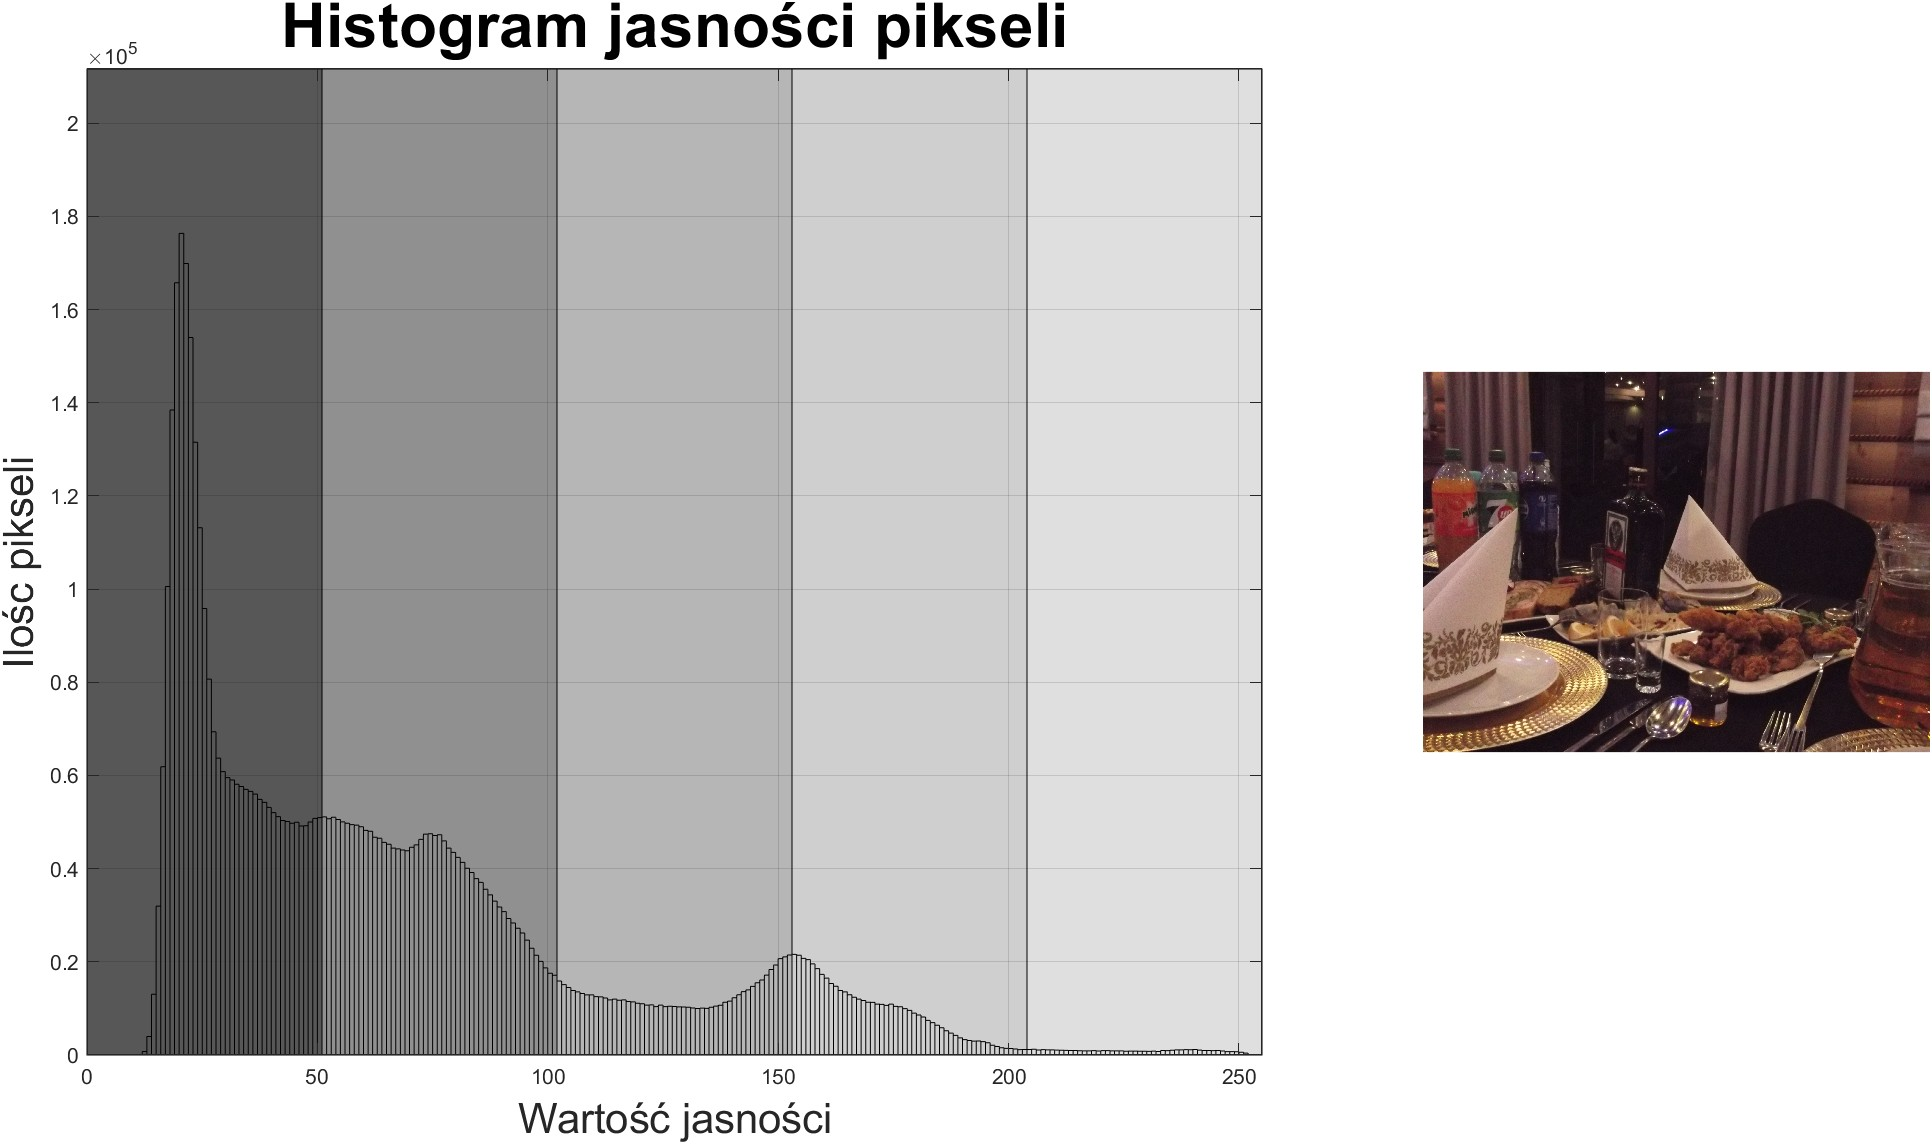
\includegraphics[width=\textwidth]{Photos1/intensity/jagier1_intensity.jpg}
\end{figure}
\begin{figure}[H]
    \centering
    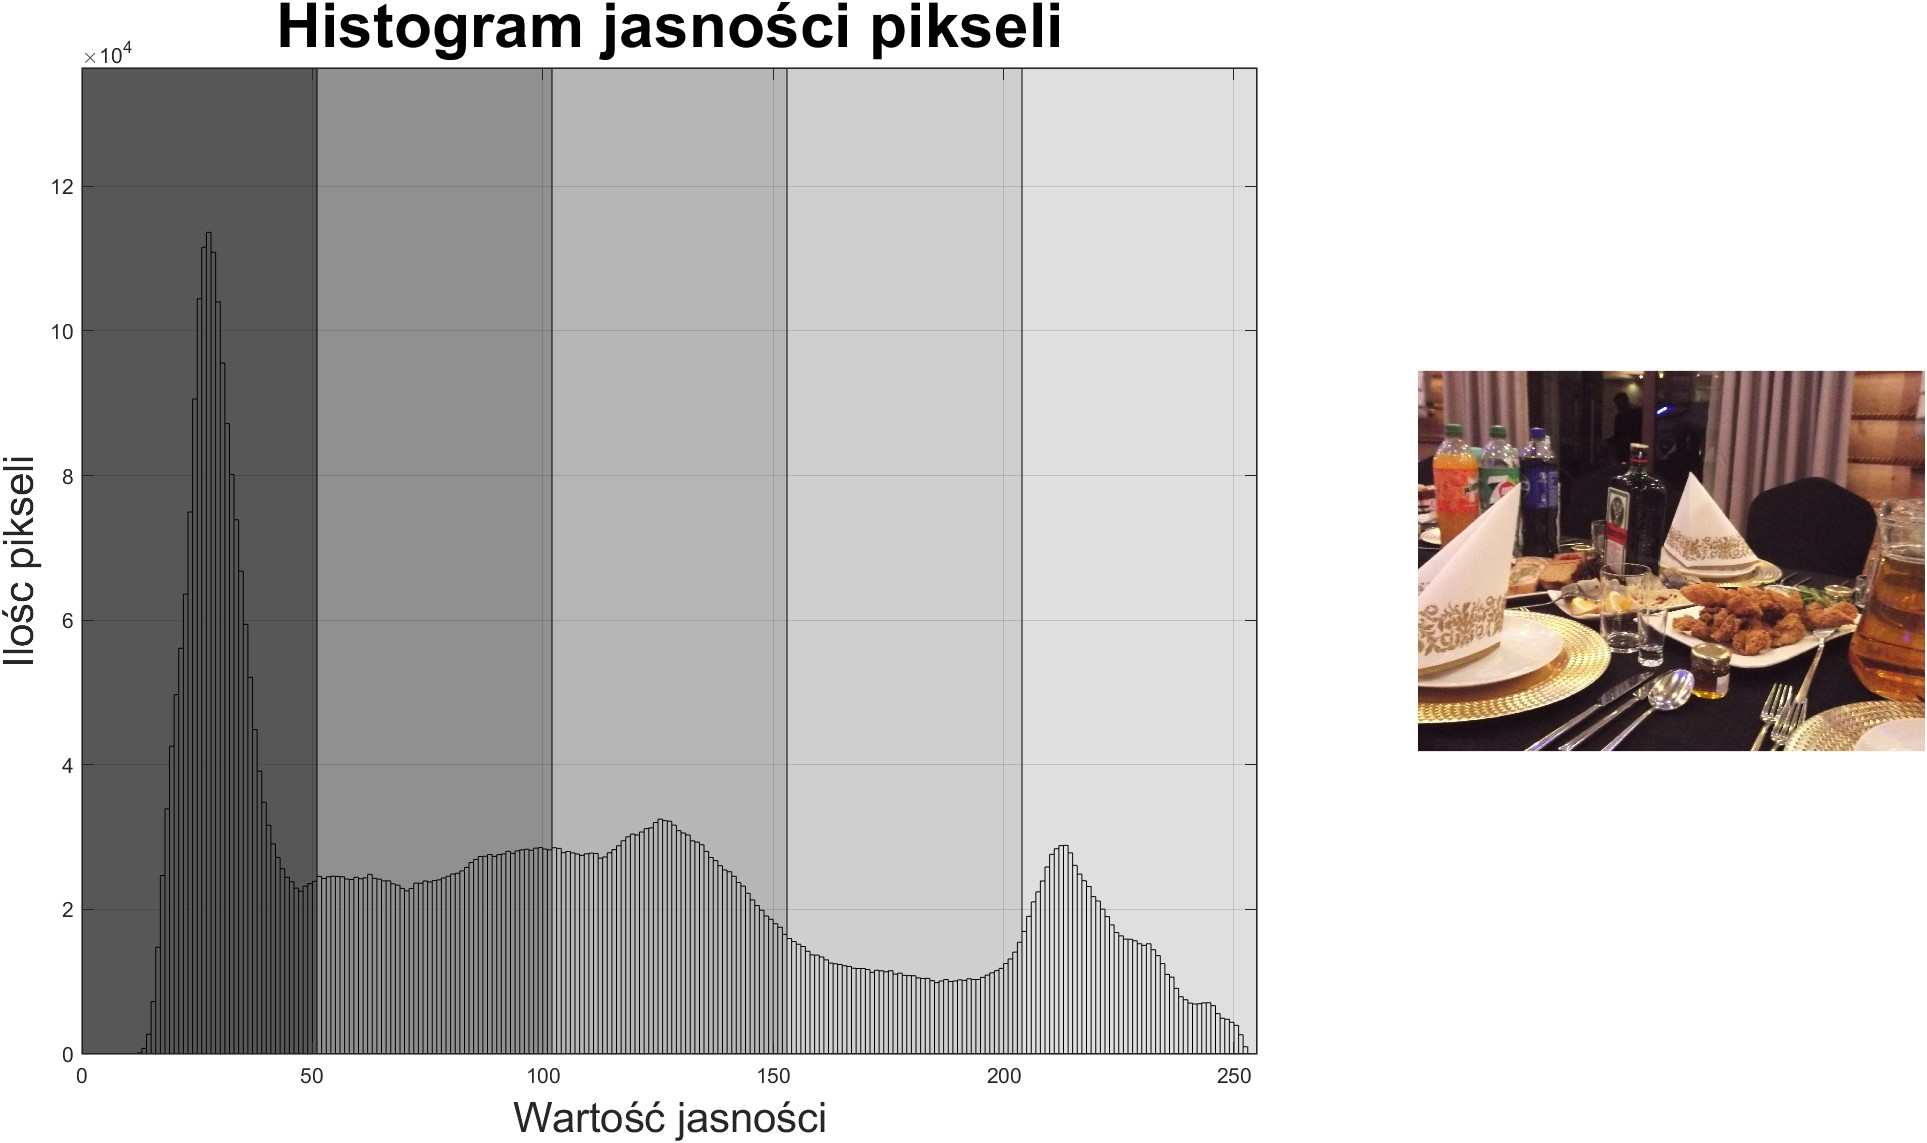
\includegraphics[width=\textwidth]{Photos1/intensity/jagier2_intensity.jpg}
\end{figure}
\begin{figure}[H]
    \centering
    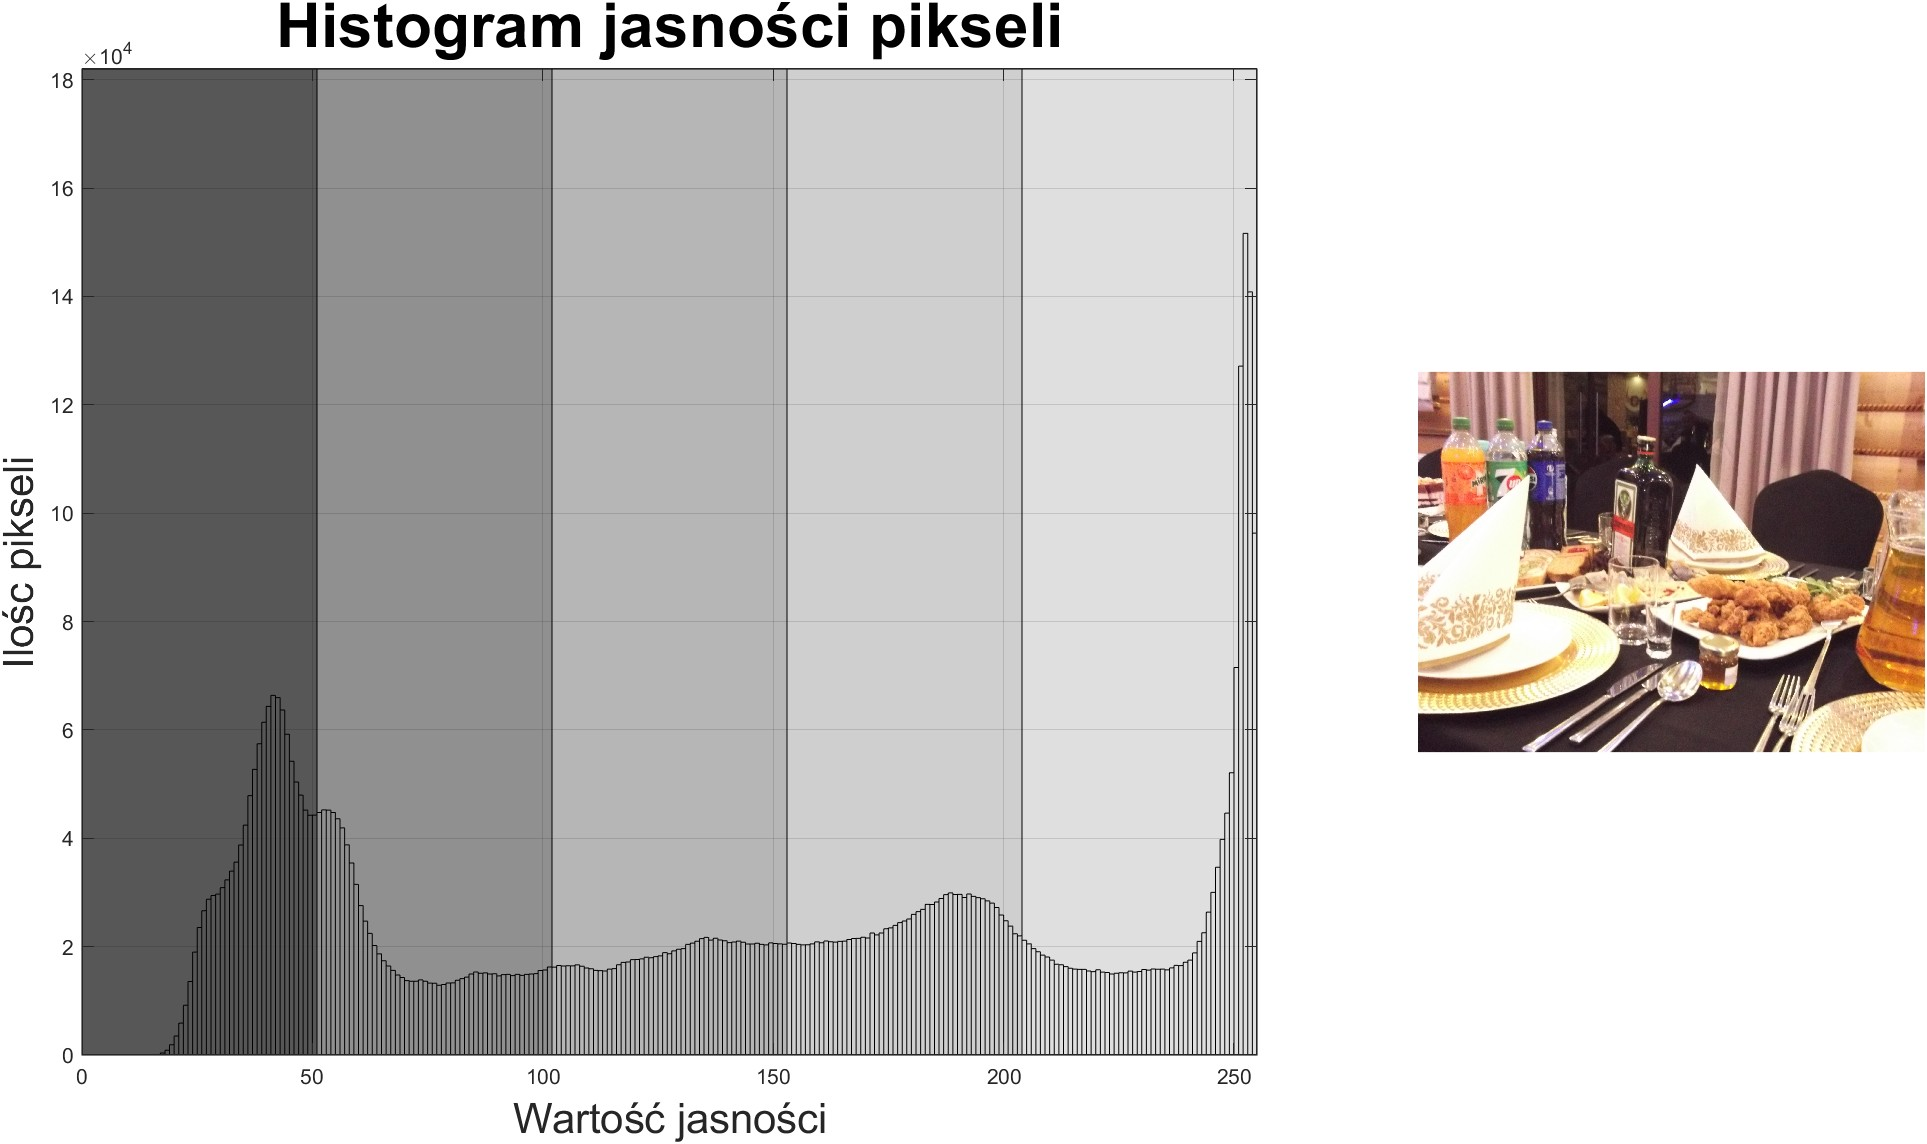
\includegraphics[width=\textwidth]{Photos1/intensity/jagier3_intensity.jpg}
\end{figure}




\newpage
\subsection{Barwa, odcień}
Hue -- z angielskiego coś pomiędzy barwą a odcieniem w fotografii odnosi się
do podstawowego koloru światła, czyli pozycji danego koloru w spektrum barw
widzialnych. Wyrażany jest w stopniach od $0$ do $360^o$ na kole
barw. Natomiast zmiana hue tylko przesuwa kolor, ale nie zmienia jego jasności
ani nasycenia. Nie badaliśmy wartości hue dla zebranych przez nas zdjęć analogowych,
ponieważ są czarno-białe. Analiza hue dla zdjęć cyfrowych pokazała nieznaczne różnice przy różnej ekspozycji.
\subsubsection{Kod}


\begin{verbatim}
    
    files = dir("photos\*.jpg");
    
    for i = 1:length(files)
    
    clear count g G im max n;
    im = imread(strcat("photos\", files(i).name));
    g = rgb2hsv(im);
    g = g(:,:,1);
    g = g*255;
    G = g(:);
    figure(1);
    set(gcf, 'Units', 'Normalized', 'OuterPosition', [0 0 1 1]); %wielkość okna
    subplot(1,3,[1,2]); 
    histogram(G,'FaceColor', '#ffffff');
    
    [count, n] = histcounts( G, 255 );
    max = max(count);
    max = max*1.2;
    
    xlim([0 255]);
    ylim([0,max]);
    
    grid on;
    title('Histogram odcienia pikseli','FontSize', 30);
    xlabel('Wartość odcienia','FontSize',20);
    ylabel('Ilośc pikseli','FontSize',20);
    
    subplot(1,3,3);
    imshow(im);
    
    exportgraphics(gcf, strcat("hue\", 
                        \\files(i).name(1:length(files(i).name)-4),"_hue.jpg"))
    close;
    
    end
    
  
    
    
    
    
    
    \end{verbatim}
\newpage


\subsubsection{Wyniki}

\begin{figure}[H]
    \centering
    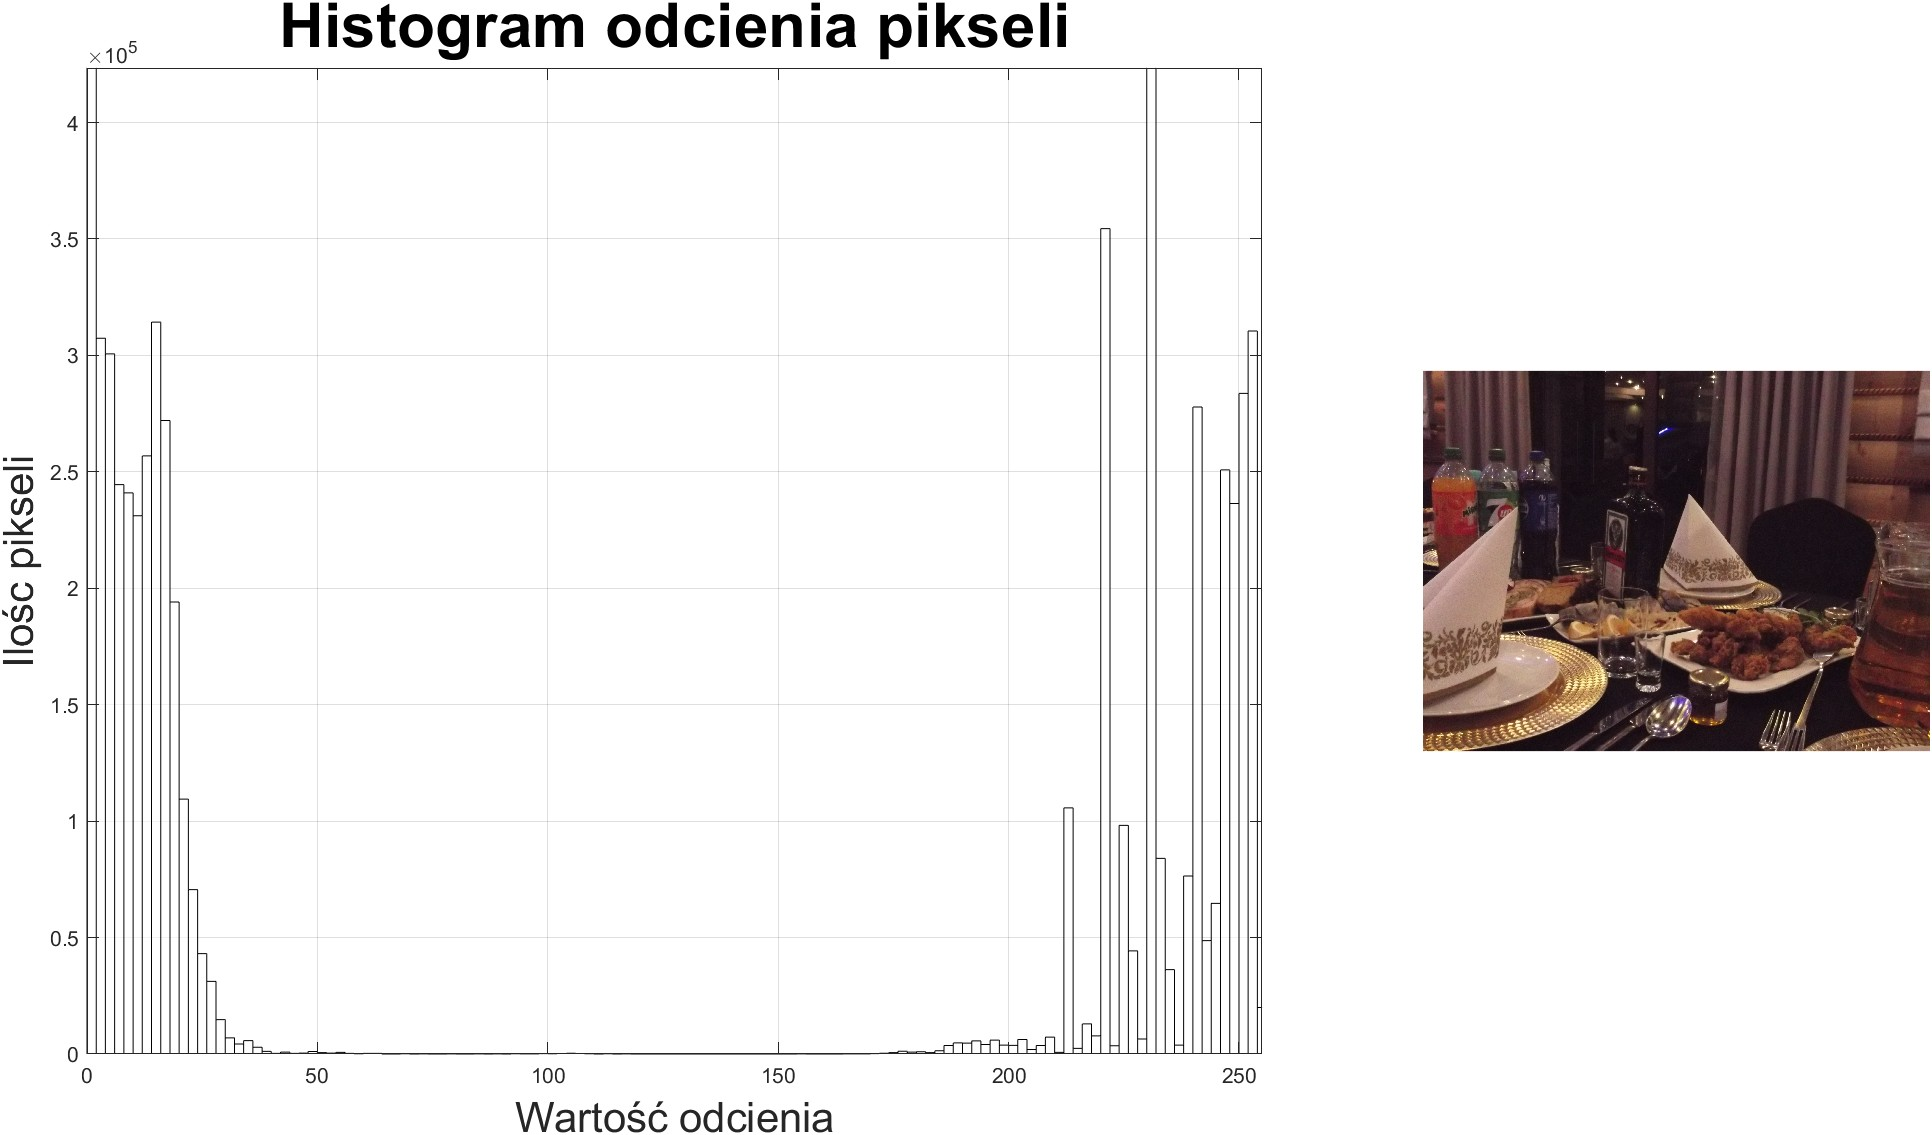
\includegraphics[width=\textwidth]{Photos1/hue/jagier1_hue.jpg}

\end{figure}
\begin{figure}[H]
    \centering
    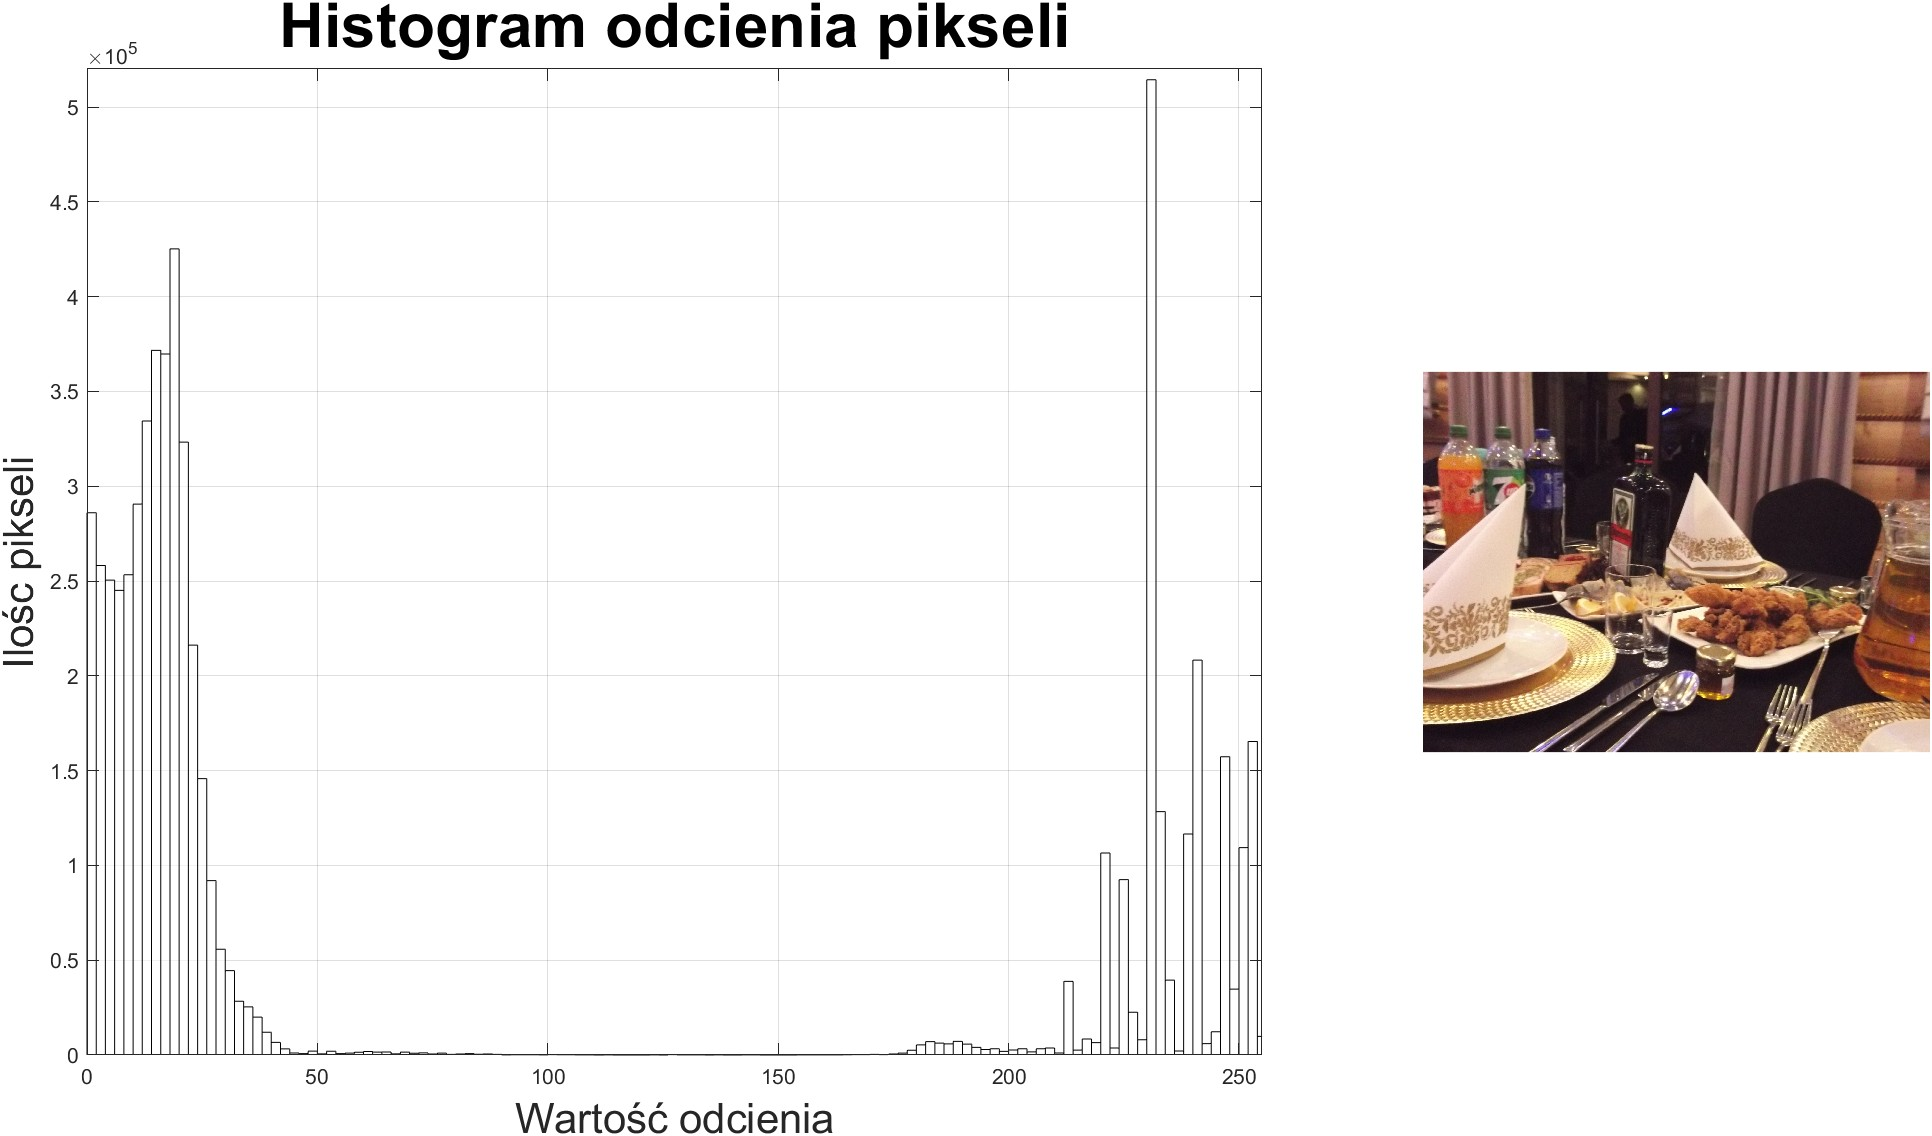
\includegraphics[width=\textwidth]{Photos1/hue/jagier2_hue.jpg}

\end{figure}
\begin{figure}[H]
    \centering
    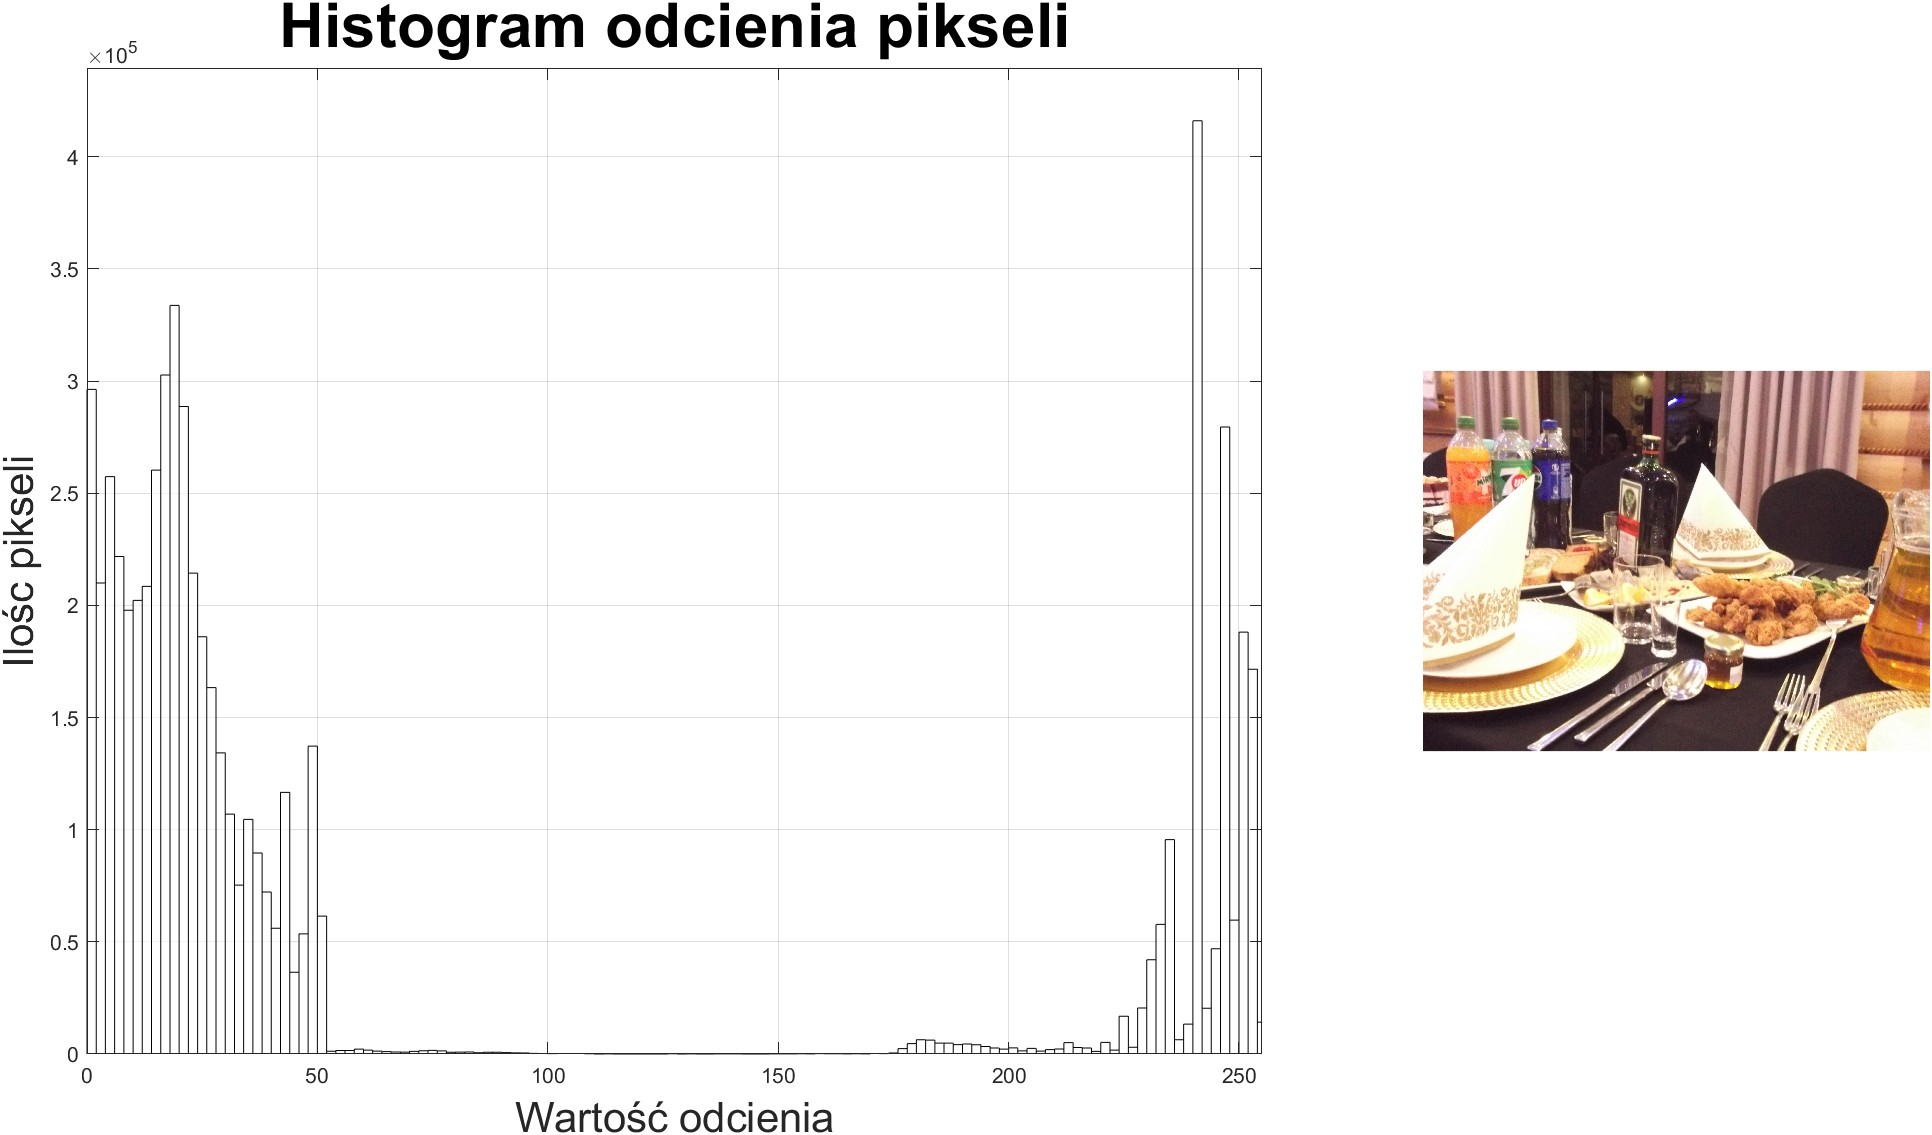
\includegraphics[width=\textwidth]{Photos1/hue/jagier3_hue.jpg}

\end{figure}



\newpage
\subsection{Saturacja}
Saturacja w fotografii to stopień intensywności kolorów na zdjęciu. Określa,
jak bardzo barwy są nasycone -- od wyblakłych i niemal czarno-białych (niska
saturacja) do bardzo żywych i intensywnych (wysoka saturacja). Tak samo jak z
hue nie badaliśmy saturacji dla zdjęć czarno-białych. Można zauważyć znaczne
różnice w saturacji zdjęć cyfrowych w zależności od stopnia naświetlenia.

\subsubsection{Kod}
\begin{verbatim}
files = dir("photos\*.jpg");

for i = 1:length(files)

clear count g G im max n;
im = imread(strcat("photos\", files(i).name));
g = rgb2hsv(im);
g = g(:,:,2);
g = g*255;
G = g(:);
figure(1);
set(gcf, 'Units', 'Normalized', 'OuterPosition', [0 0 1 1]); %wielkość okna
subplot(1,3,[1,2]); 
histogram(G,'FaceColor', '#ffffff');

[count, n] = histcounts( G, 255 );
max = max(count);
max = max*1.2;

xlim([0 255]);
ylim([0,max]);

grid on;
title('Histogram nasycenia pikseli','FontSize', 30);
xlabel('Wartość nasycenia','FontSize',20);
ylabel('Ilośc pikseli','FontSize',20);

subplot(1,3,3);
imshow(im);

exportgraphics(gcf, strcat("saturation\", 
            \\files(i).name(1:length(files(i).name)-4),"_saturation.jpg"))
close;

end

\end{verbatim}

\newpage
\subsubsection{Wyniki}


\begin{figure}[H]
    \centering
    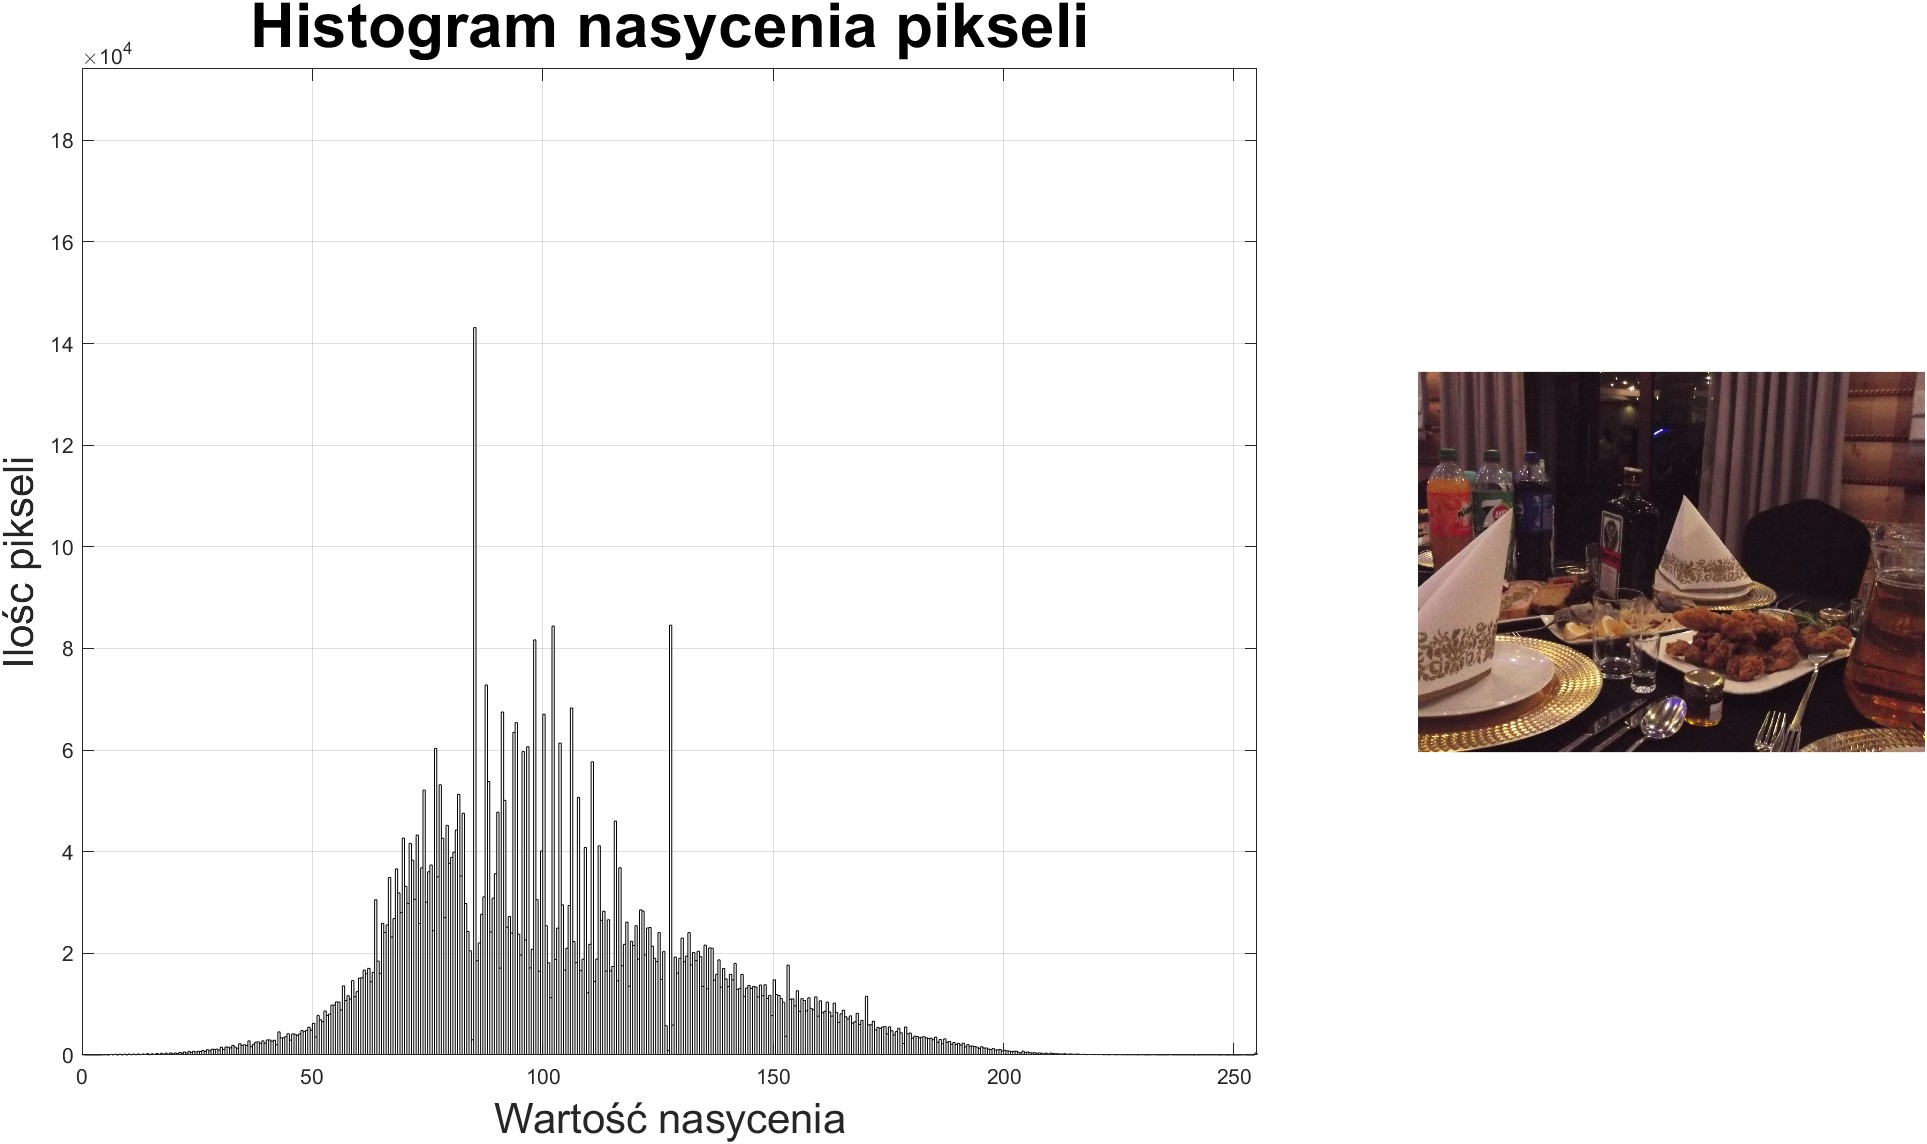
\includegraphics[width=\textwidth]{Photos1/saturation/jagier1_saturation.jpg}

\end{figure}
\begin{figure}[H]
    \centering
    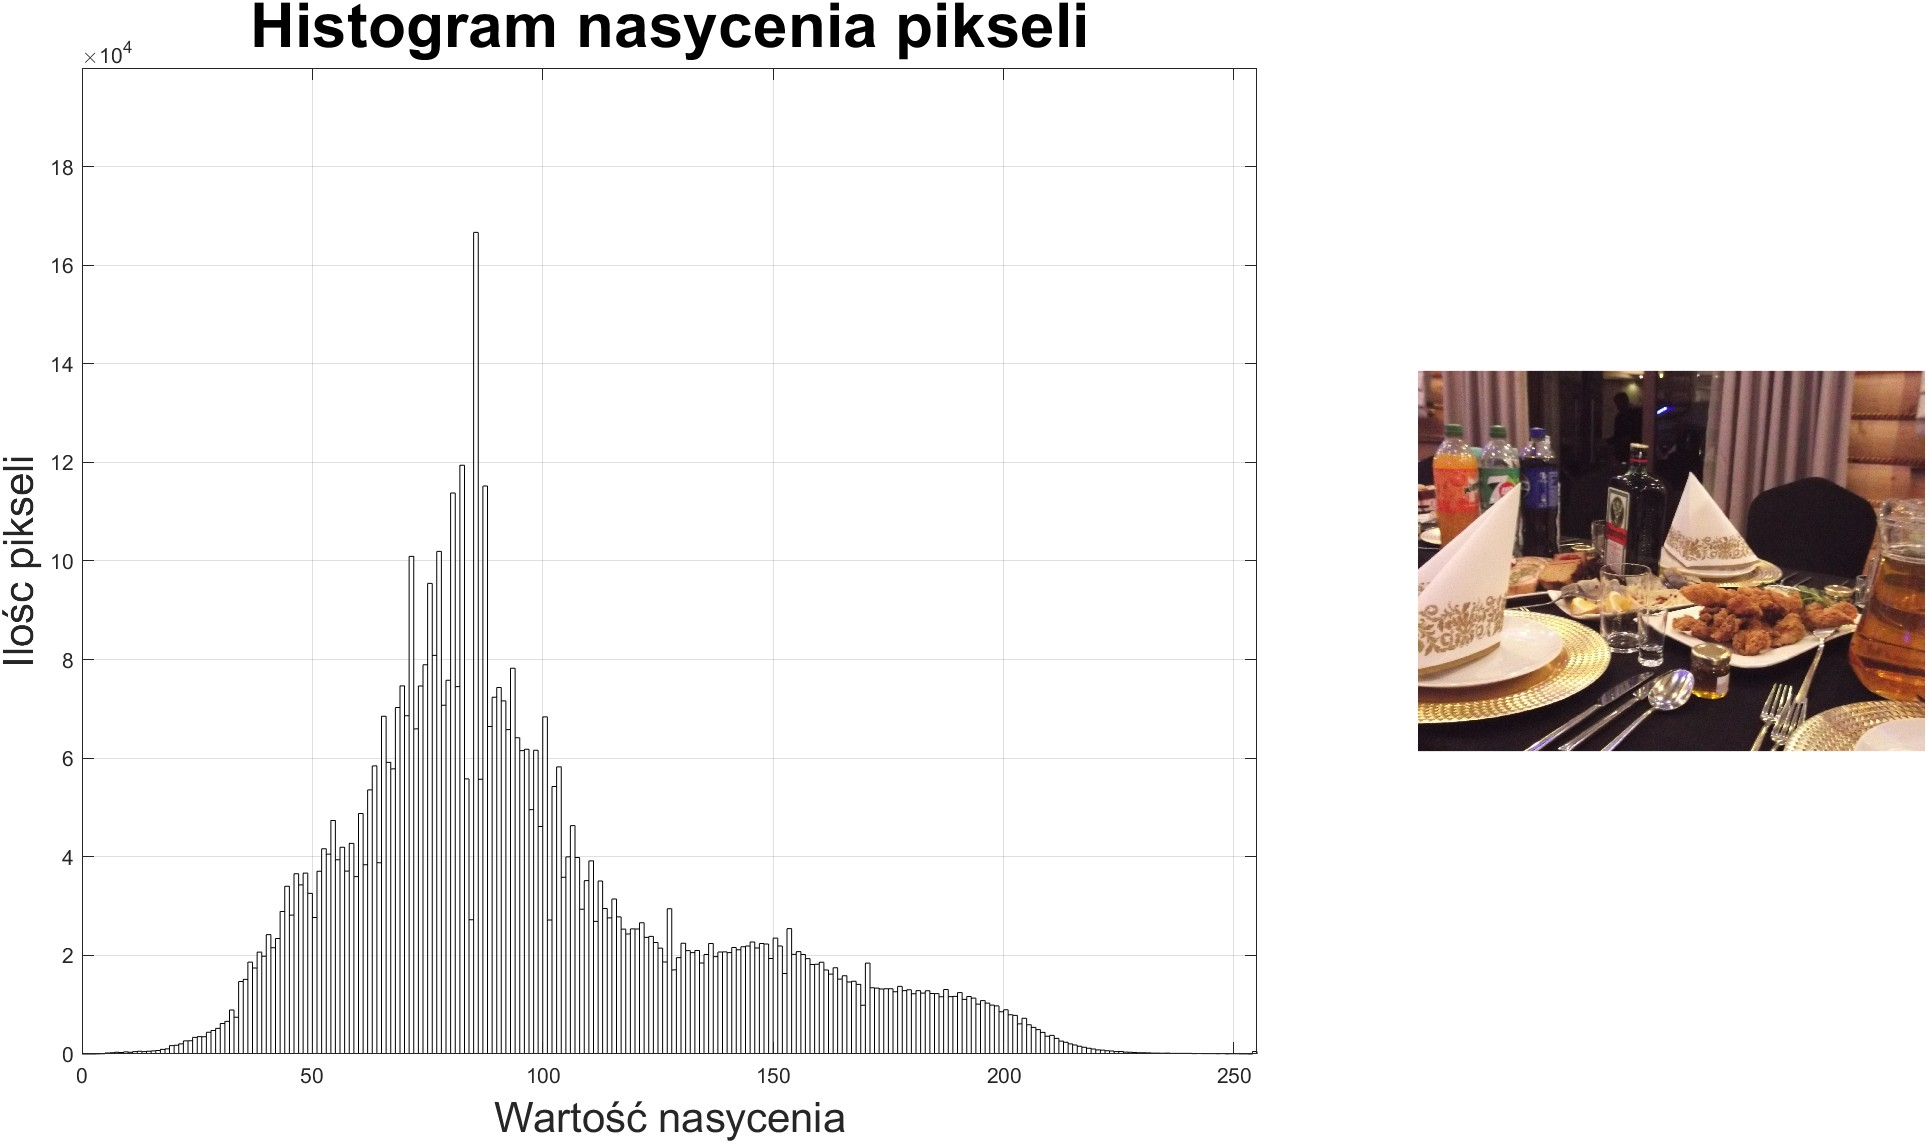
\includegraphics[width=\textwidth]{Photos1/saturation/jagier2_saturation.jpg}

\end{figure}
\begin{figure}[H]
    \centering
    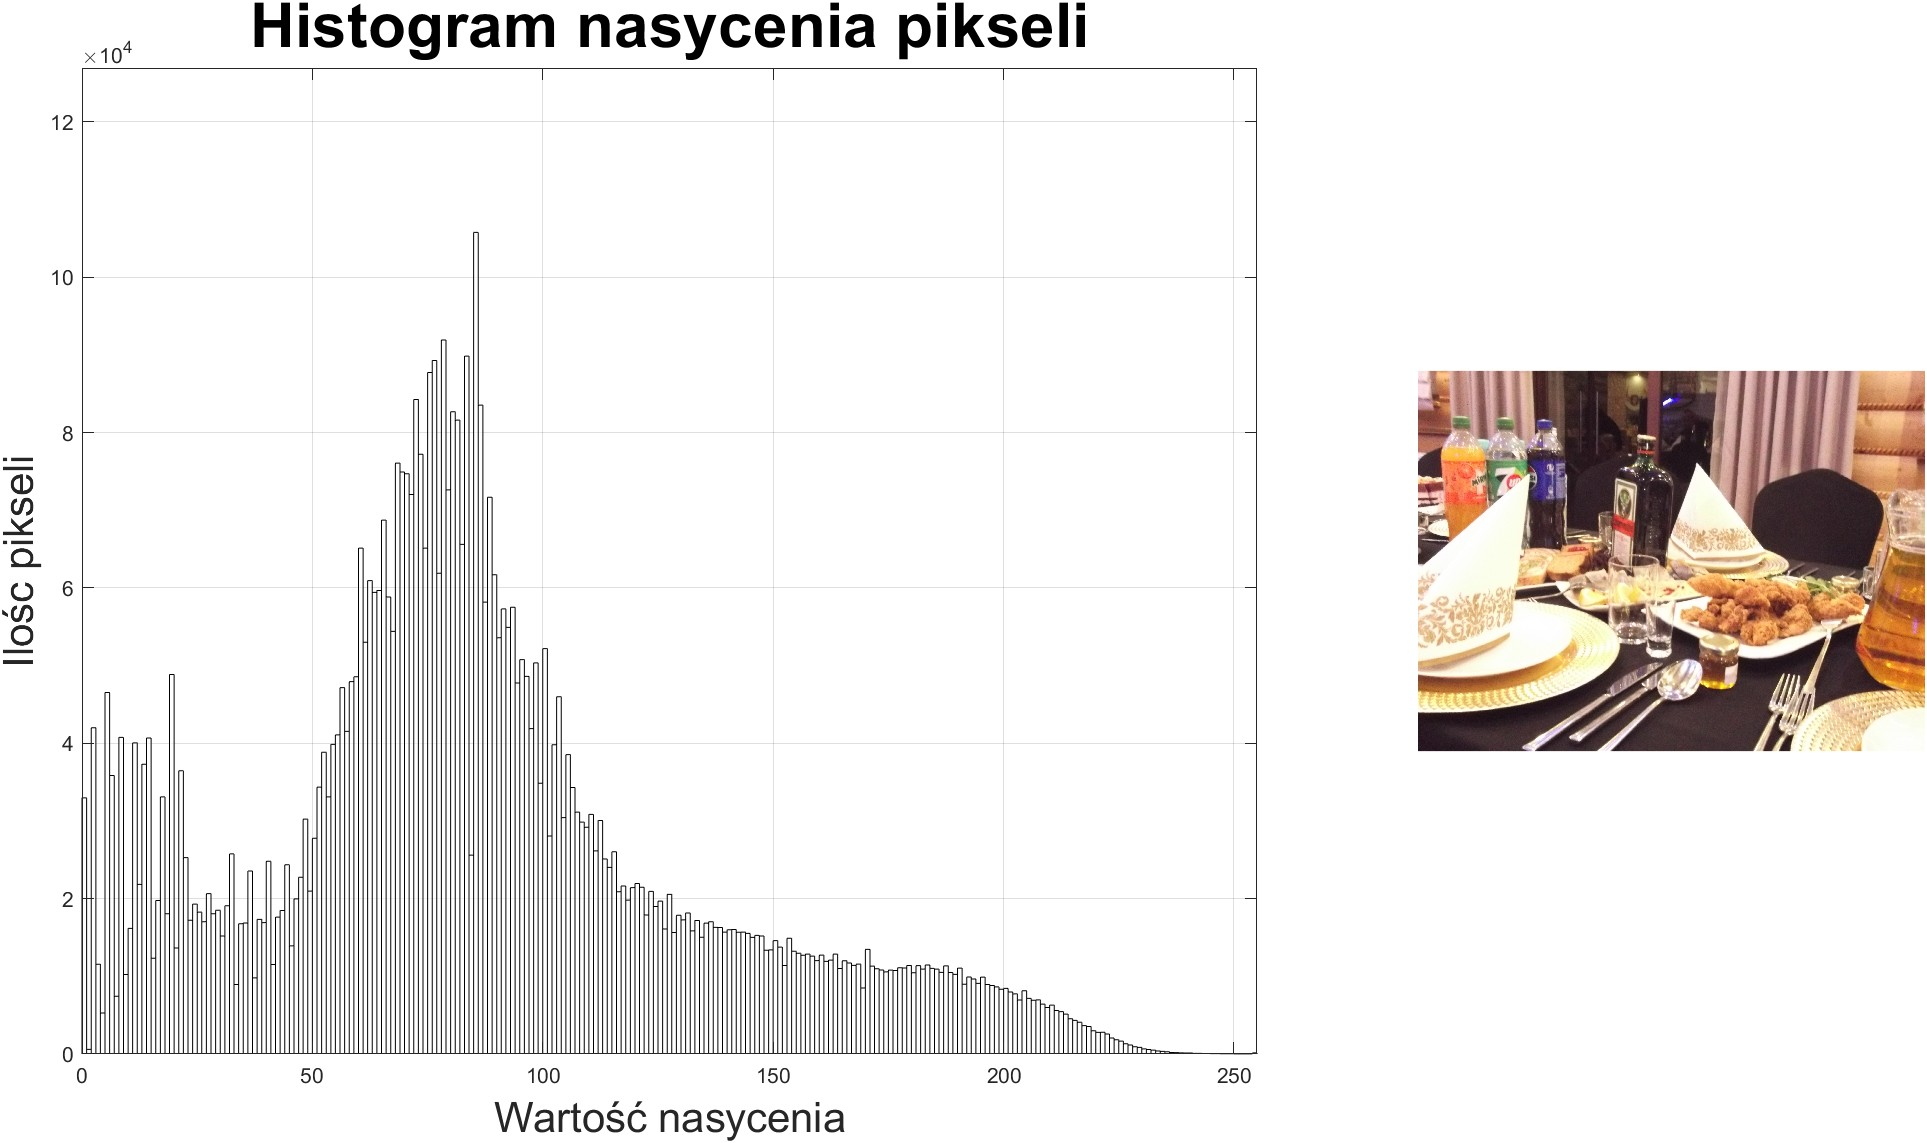
\includegraphics[width=\textwidth]{Photos1/saturation/jagier3_saturation.jpg}

\end{figure}

\newpage



\newpage
\subsection{Kontrast}
Kontrast w fotografii to różnica między jasnymi i ciemnymi obszarami zdjęcia.
Określa, jak bardzo elementy obrazu różnią się od siebie pod względem
jasności, koloru lub tonu. Wyższy kontrast sprawia, że zdjęcie wygląda
bardziej dynamicznie, a niski kontrast daje bardziej miękki, wyblakły
efekt.

\subsubsection{Kod}
\begin{verbatim}
    files = dir("photos\*.jpg");
cont = struct('plik', cell(1,length(files)), 'kontrast',
                \\cell(1,length(files)), 'jasnosc', cell(1,length(files)));

for i = 1:length(files)

clear g G l im j k m n R;
im = imread(strcat("photos\", files(i).name)); 
g = rgb2gray(im);
g = single(g);
g=g/255;
G = g(:);
I = mean(G);
[n, m] = size(g);
R =0.0;

for k=1:1:n
    for j = 1:1:m
        R = R + (g(k,j) - I)^2;
    end
end

R = R/(m*n);

R = sqrt(R);

%disp(["Kontrast zdjęcia" R]);
%disp(["Średnia jasność zdjęcia" I]);

cont(i).plik = files(i).name;
cont(i).kontrast = R;
cont(i).jasnosc = I;

end

writetable(struct2table(cont), 'contrast.csv')

\end{verbatim}
\subsubsection{Wyniki}
Co w przypadku naszego zdjęcia dało wyniki następujące:

\begin{table}[h]
    \centering
    \begin{tabular}{|c|c|c|}
        \hline
        Zdjęcie                      & Kontrast  & Jasność    \\ \hline
        Zdjęcie stołu niedoświetlone & 0.1856783 & 0.2637069  \\ \hline
        Zdjęcie stołu idealne        & 0.2608515 & 0.39802570 \\ \hline
        Zdjęcie stołu prześwietlone  & 0.3019148 & 0.54119000 \\ \hline
    \end{tabular}
    \caption{Wyniki dla używanego w raporcie przykładowego zdjęcia stołu}
\end{table}

\newpage
\subsection{Wnioski i plany na przyszłość}
Analiza danych zebranych w powyższych częściach okazała się trudnym zadaniem,
dlatego wrócimy do niej w kolejnym raporcie. Zamieszczamy jednak poniższą tablę,
której poprawności statystycznej dla ogółu danych nie jesteśmy pewni. Na podstawie
danych jesteśmy wciąż w stanie postawić hipotezę, że: im większe doświetlenie tym
wyższy kontrast i jasność. nirzsze


\begin{table}[h]
    \centering
    \begin{tabular}{|c|c|c|c|c|c|}
        \hline
        EV       & -1    & $+\delta$ & 0     & $+\delta$ & +1    \\ \hline
        Kontrast & 0.119 & +37 \%    & 0.163 & +26 \%    & 0.206 \\ \hline
        Jasność  & 0.231 & +27 \%    & 0.294 & +20 \%    & 0.352 \\ \hline
    \end{tabular}
    \caption{Średnie jasności i kontrastu od korekty naświetlenia}

\end{table}




\section{Wykorzystywane narzędzia}
W tej części naszego projektu korzystaliśmy z następujących narzędzi:
\begin{itemize}
    \item Programu Matlab -- do analizy zdjęć;
    \item Programu LibreOffice Calc -- do analizy wyników ankiety;
    \item $\LaTeXe{}$ -- do przygotowania raportu;
    \item Google Drive -- do udostępniania plików;
    \item 7zip -- do kompresji zdjęć;
    \item Aparatów:
          \begin{itemize}
              \item Canon EOS 300 z obiektywem Tamron 28-105mm 1:4-5.6 i kliszą Fomapan 400
              \item Fujifilm FinePix L55 Digital Camera -- Black (12MP, 3x Optical Zoom)
          \end{itemize}
\end{itemize}


\section{Podział obowiązków}
Po wyborze celu projektu wszyscy zajęliśmy się zdobywaniem wiedzy na
temat problemów fotografii analogowej, a także możliwych poprawy jakości zdjęć.\newline


Posiadając wstępną wiedzę na temat materii projektu organicznie wstępnie
podzieliliśmy się zajęciami zgodnie z naszymi zainteresowaniami: \newline
\begin{itemize}
    \item pozyskiwanie materiałów testowych -- Aleksandra Wójcik, Bartosz Wójcik;
    \item opracowanie skryptów do analizy zdjęć i zbieranie informacji do algorytmu -- Katarzyna Szwed, Karol Sęk, Michał Juszkiewicz;
    \item opracowywanie raportu -- Patrycja Szałajko, Natalia Szymańska, Filip Sajko.
\end{itemize}

\newpage































































































\part{}
\thispagestyle{empty}

\begin{figure}[h]
    \centering
    
\includegraphics[width=1\textwidth]{wspolne_dla_wszystkich/logo_uczelni.png}
\end{figure}


\begin{center}
    {\LARGE \textbf{Poprawa jakości skanów zdjęć wykonanych techniką analogową
        }} \\[0.3cm]
    {\large \textbf{Raport II}} \\[0.2cm]
    \textit{projekt realizowany pod opieką prof. dr hab. inż. Artura Przelaskowskiego}

\end{center}

\begin{figure}[h]
    \centering
    
\includegraphics[width=1\textwidth]{wspolne_dla_wszystkich/logo_projektu.png}
\end{figure}

\vfill
\begin{abstract}
    Raport 2 projektu poprawy jakości cyfrowych skanów zdjęć wykonanych techniką analogową przez grupę nr 9 (wtorkową z godziny 18)
    w składzie:  Bartosz Wójcik, Katarzyna Szwed, Natalia Szymańska,
    Patrycja Szałajko, Aleksandra Wójcik, Karol Sęk, Michał Juszkiewicz, Filip Sajko.

    W tym raporcie zredefiniujemy cel naszego projektu i opiszemy problem z którym się mierzymy.
    Przedstawimy ponadto wstępną wersję naszego programu i zademonstrujemy jego skuteczność.
\end{abstract}


\newpage

% ADD KOREKTA
\section{Korekta do raportu 1}
\begin{itemize}
    \item Do skanowania zdjęć w pierwszym etapie projektu użyty był skaner minilab Noritsu HS-1800.
    \item Zdjęcia były robione przy różnych ustawieniach Exposure Value, za zdjęcia niedoświetlone uznaliśmy te robione przy EV-1, a za prześwietlone przy EV+1.
    \item Również doprecyzowaliśmy tytuł projektu.
\end{itemize}


\section{Cel projektu}
W związku ze słusznymi uwagami i wskazówkami, podjęliśmy decyzję o ukonkretyzowaniu celu naszego projektu.
Skupimy się przede wszystkim na poprawianiu defektów cyfrowych skanów zdjęć analogowych.
Na ten moment pracowaliśmy nad usuwaniem artefaktów powstałych w procesie wywoływania zdjęć i naprawianiem kontrastu zdjęć.
Naszym celem jest zarówno naprawienie jakości starych zdjęć rodzinnych,
jak i tych robionych przez współczesnych amatorów fotografii analogowej.

\section{Zdjęcia, zdjęcia!}
Profilowym zdjęciem dla nas jest portret -- tak indywidualny jak i grupowy.
Jest to typ zdjęć najbardziej popularny w rodzinnych albumach -- mnogość w nich zdjęć z ważnych
dla danej familli wydarzeń: chrztów, wesel czy pogrzebów... Służą one utrwaleniu wspomnień oraz pamięci
po krewnych i bliskich, którzy już odeszli... A więc noszących dużą wartość emocjonalną dla ich posiadacza.

Nasza koleżanka Ola odnalazła stary album rodzinny i zeskanowała znajdujące się w nim zdjęcia.
Docelowo zajmiemy się naprawianiem skanów właśnie tych zdjęć.
Często pojawiającymi się problemami wśród tych zdjęć są niedoświetlenie oraz zagięcia.

\begin{figure}[H]
    \centering
    \includegraphics[width=\linewidth, keepaspectratio]{Photos2/STARE/Scan2025-04-14_101906.png}
    \caption{Przykładowe zdjęcie z albumu, który można znaleźć \href{https://drive.google.com/drive/folders/1FME2DGxQ3jP6B-MKmGzHXzVHgdVP4-Fq}{tutaj!} }
\end{figure}

\newpage
\section{Problemy}
Wykonywanie, a następnie `ucyfrowienie' zdjęcia w technice analogowej wiąże się z różnymi trudnościami,
które mogą znacząco obniżyć jakość zdjęcia -- a z tym satysfakcje jego posiadacza. Głównymi problemami,
którym będziemy przeciwdziałać, będą niedoświetlenie zdjęcia i zanieczyszczenia powietrza osadzające
się na oryginalnym zdjęciu i skanerze podczas procesu zmiany informacji z analogowej na cyfrową.

\subsection{Niedoświetlenie} % tak wiem bartek bedziesz krzyczał. ale poezja to poezja, e viva latre
Niedoświetlenie jest problemem trudnym -- zwłaszcza dla fanów-amatorów techniki analogowej.
Zasadnicza większość klasycznych aparatów nie posiada zaawansowanej mechaniki automatycznie wybierającej
odpowiednie ustawienia aparatu, a brak możliwości podglądu tego, jak dane zdjęcie wyszło, często doprowadza
do sytuacji, gdzie po wielu dniach okazuje się, że na zdjęciu chwili, którą fotograf chciał uchwycić i utrwalić,
niewiele widać, bo przez złe ustawienia większość szczegółów jest niewidoczna. Jest to problem, który szeroko
wraz z przykładami i analizą numeryczną opisywaliśmy w raporcie pierwszym.

Dla przykładu przypomnijmy:
\newpage
\begin{figure}[H]
    \centering
    \includegraphics[angle=90, width=\linewidth, keepaspectratio]{Photos2/doswietlone_i_nie/analog6.jpg}
    \caption{Zdjęcie niedoświetlone.}
\end{figure}
\begin{figure}[H]
    \centering
    \includegraphics[angle=90, width=\linewidth, keepaspectratio]{Photos2/doswietlone_i_nie/analog7.jpg}
    \caption{...i to w punkt.}
\end{figure}


% REWORD THIS 

\newpage
\subsection{Artefakty}
Artefakty na zdjęciach analogowych powstają ze względu na osadzanie się kurzu i innych zanieczyszczeń na wywołanej kliszy,
a także przez jej zarysowanie.

Przez to na negatywie powstają ciemne plamki, które w momencie powstawania odbitki z kolei zamieniają się w jasne plamy.

Takie zjawisko można zaobserwować na poniższych zdjęciach:

\begin{figure}[H]
    \centering
    \includegraphics[width=\linewidth, keepaspectratio]{Photos2/przed/GRAYgpt3.png}
    \caption{W skrajnych wypadkach może wyglądać to nawet tak.}
\end{figure}

\begin{figure}[H]
    \centering
    \includegraphics[width=\linewidth, keepaspectratio]{Photos2/przed/new1.jpeg}
    \caption{Choć bardziej częstym jest ten przypadek.}
\end{figure}

\begin{figure}[H]
    \centering
    \includegraphics[width=\linewidth, keepaspectratio]{Photos2/przed/new2.jpeg}
    \caption{A także taki.}
\end{figure}

\newpage
\section{Program i jego działanie}
Zbrojni w wiedzę co chcemy osiągnąć i zapas zebranych skanów zdjęć do testów wzięliśmy się do pracy
nad programem. Stworzyliśmy zaawansowany program, który inteligentnie przeszukuje cały obszar zdjęcia, zaznacza artefakty,
a w następnej fazie działania usuwa je. Warto dodać, że algorytm przekształca zdjęcie z formatu RGB do formatu HSV (Hue, Saturation, Value) i działa tylko na Value,
która definiuje jasność piksela w skali 0-255.

Przechodząc do szczegółów, działanie programu można opisać za pomocą kilku kolejnych faz działania, na przykładzie poniższego zdjęcia:

\begin{figure}[H]
    \centering
    \includegraphics[width=\linewidth, keepaspectratio]{Photos2/przed/gpt1.png}
    \caption{Przykładowe zdjęcie -- to za jego pomocą opiszemy działanie programu.}
\end{figure}


\subsection{Tworzenie maski}
\subsubsection{Rozmycie gaussowskie}
Pierwszym krokiem generowania maski jest stworzenie rozmycia gaussowskiego zdjęcia.

Wygładzanie gaussowskie jest efektem rozmywania obrazu za pomocą funkcji Gaussa,
która jest szeroko wykorzystywana w grafice komputerowej w celu uzyskania gładkiego
wygładzenia obrazu i wyciszenia szumu informacyjnego.

Za pomocą funkcji danej wzorem dla każdego piksela:
\begin{equation}
    G(x, y) = \frac{1}{2 \pi \sigma^2}e^{- \frac{x^2+y^2}{2\sigma^2}}
\end{equation}
gdzie $x$, $y$ to współrzędne danego piksel'a, a $\sigma$ oznacza odchylenie standardowe.\footnote{Źródło: \url{https://en.wikipedia.org/wiki/Gaussian_blur}}

\begin{figure}[H]
    \centering
    \includegraphics[width=\linewidth, keepaspectratio]{Photos2/gauss_blurr/gauss_blurr_gpt1.png}
    \caption{Zdjęcie po wykonaniu rozmycia gaussowskiego.}
\end{figure}

\subsubsection{Wykonanie różnicy}
Następnie odejmujemy od oryginału zdjęcia otrzymane w poprzednim etapie rozmycie.
Pozwala to na wykrycie najbardziej kontrastowych elementów zdjęcia.

\begin{figure}[H]
    \centering
    \includegraphics[width=\linewidth, keepaspectratio]{Photos2/difference/difference_gpt1.png}
    \caption{Zdjęcie po wykonaniu różnicy.}
\end{figure}

\subsubsection{Usunięcie ciemnych pikseli}
Zostawiamy tylko jasne piksele (według standardowych ustawień jest
to jasność powyżej 60) i nadajemy im maksymalną wartość 255.
Pozostałym pikselom ustawiamy jasność na 0.

\newpage
\subsubsection{Korekcja gamma}

Korekcja gamma jest techniką stosowaną w grafice komputerowej, której celem jest dostosowanie
jasności obrazu do ludzkiego nielinowego postrzegania światła. Korekcja gamma kompensuje ten
nieliniowy sposób widzenia, pozwalając na efektywniejsze wykorzystanie dostępnych poziomów jasności.

Korekcja gamma dokonuje transformacja jasności w następujący sposób:
\begin{equation}
    L'(x,y) = L(x,y)^{\gamma}
\end{equation}
gdzie:
\begin{itemize}
    \item $\gamma$ to współczynnik gamma,
    \item $L(x,y)$ to wartości jasności pikseli.
\end{itemize}

Wiedząc to, w tym etapie bierzemy ponownie oryginalne zdjęcie, wykonujemy
na nim korekcję gamma, a następnie na tym zdjęciu wykonujemy etapy 1-3.

Działanie to pozwala uwzględnić jak najwięcej artefaktów
-- znajdujących się także na jasnym tle.

\begin{figure}[H]
    \centering
    \includegraphics[width=\linewidth, keepaspectratio]{Photos2/gamma_corection/gamma_corection_gpt1.png}
    \caption{Po wykonaniu korekcji gamma i etapów 1-3.}
\end{figure}

\newpage
\subsection{Gotowa maska}
Po tym wszystkim otrzymujemy dwie podmaski (jedna robiona na oryginalnym
zdjęciu, a druga na jaśniejszym -- rozświetloną modulacją gamma).
Końcową maskę otrzymujemy biorąc wszystkie znalezione piksele z obu podmasek.

\begin{figure}[H]
    \centering
    \includegraphics[width=\linewidth, keepaspectratio]{Photos2/masks/final_mask_gpt1.png}
    \caption{Maska wykonana z oganianego zdjęcia}
\end{figure}
\begin{figure}[H]
    \centering
    \includegraphics[width=\linewidth, keepaspectratio]{Photos2/masks/second(gc)_mask_gpt1.png}
    \caption{Maska wykonana z zdjęcia rozświetlonego korekcją gamma}
\end{figure}


\newpage
\subsection{Działanie właściwe}
Mając wygenerowaną maskę właściwą, przechodzimy po wyznaczonych
przez nią pikselach na oryginalnym zdjęciu. Dla każdego piksela w
zaznaczonego w masce wyliczamy nową wartość jasności -- średnią z
jasności wszystkich (nie zaliczają się do tego pikseli wyznaczone
wcześniej przez maskę.) pikseli na odległości nie więcej 15 od aktualnie analizowanego.

Wynik finalny:
\begin{figure}[H]
    \centering
    \includegraphics[width=\linewidth, keepaspectratio]{Photos2/przed/gpt1.png}
    \includegraphics[width=\linewidth, keepaspectratio]{Photos2/po/gpt1.png}
    \caption{Przykładowe zdjęcie -- porównanie efektu przed i po.}

\end{figure}

\newpage
\section{Uwagi co do działania programu}
Przez to, że algorytm działa lokalnie (tylko w punktach wyznaczonych
przez maskę) nie wpływa on na ogólny wygląd zdjęcia.
Z tego też powodu możemy wykonywać program kilkukrotnie na zdjęciu
-- uzyskując lepsze efekty.

Końcowy algorytm składa się z pięciu iteracji opisanego wyżej algorytmu,
znacząco zwiększając szansę na usunięcie zanieczyszczeń.

Ponadto można uzyskać dodatkowe informacje o działaniu programu
i jakości zdjęcia -- za przykład funkcja: .countNoise()
zlicza ilość wyznaczonych przez maskę pikseli -- które są uznane za zanieczyszczenia.


\section{Program do zmiany kontrastu zdjęcia}
Napisaliśmy też osobny program zmieniający kontrast obrazu.
Użyliśmy języka Matlab ze względu na to, że umożliwia on łatwiejsze porównanie wyników ze względu na parametr gamma.
Algorytm korzysta z korekcji gamma opisanej wcześniej w punkcie 4.1.4.

\subsection{Kod}
\begin{verbatim}
g = imread("test_2.png");
figure(1);
tiledlayout(3,3)
nexttile
imshow(g);
title("zdjęcie niezmienione")
gamma = 0.25;
for k=1:9
    if gamma ~= 1
        gout = double(g)/255;
        gout = gout.^gamma;
        gout = gout*255;
        gout = uint8(gout);
        nexttile
        imshow(gout);
        title(['gamma = ' num2str(gamma)]);
    end
    gamma = gamma + 0.25;
end
\end{verbatim}

\newpage
\subsection{Działanie programu ze względu na parametr gamma}
%tutaj zdjęcie co wysłałam na discordzie
\begin{figure}[H]
    \centering
    \includegraphics[width=\textwidth, keepaspectratio]{Photos2/porownanie.png}
    \caption{Działanie programu dla różnych parametrów $\gamma$}
\end{figure}


\section{Dalsze kroki}
Na chwilę obecną nasze rozwiązanie jest programem terminalowym,
działającym na systemie nie starszym niż Windows 10 -- choć istnieje
plan przeniesienia go także na inne popularne systemy operacyjne.

Tak samo pracujemy obecnie nad stworzeniem bardziej przystępnego interfejsu okienkowego, a przy tym
planujemy integrację poszczególnych elementów programu. Zamierzamy również między innymi dodać funkcjonalność usuwającą widoczne zagięcia.

Program dostępny jest na licencji \textit{open source} i jego kod źródłowy można znaleźć na GitHubie
pod adresem:
\begin{center}
    \url{https://github.com/ssk12o/PTI-Foto-Projekt}.
\end{center}




\newpage
\section{Wykorzystywane narzędzia}
W tej części naszego projektu korzystaliśmy z następujących narzędzi:
\begin{itemize}
    \item Programu i języka Matlab -- do analizy zdjęć i kontrastu;
    \item Języka C++ -- do napisania programu usuwającego artefakty;
    \item Programu VS Code -- do tworzenia, edycji i dokumentacji kodu programu i raportów;
    \item Programu LibreOffice Calc -- do analizy części danych numerycznych;
    \item $\LaTeXe{}$ -- do przygotowania raportu;
    \item Strony Github i programu Git -- do udostępniania, dystrybucji i pracy nad kodem;
    \item 7zip -- do kompresji zdjęć;
    \item Google Drive -- do udostępniania plików;
    \item Skanera minilab Noritsu HS-1800 -- do wykonywania wysokiej jakości cyfrowych skanów zdjęć wykonanych techniką analogową;
    \item Aparatów:
          \begin{itemize}
              \item Canon EOS 300 z obiektywem Tamron 28-105mm 1:4-5.6 i kliszą Fomapan 400
              \item Fujifilm FinePix L55 Digital Camera -- Black (12MP, 3x Optical Zoom)
          \end{itemize}
\end{itemize}


\section{Podział obowiązków}
Na tym etapie projektu podzieliśmy się pracą, obowiązkami i zadaniami w następujący sposób:
\begin{itemize}
    \item Bartosz Wójcik -- wykonywanie, skanowanie i analiza zdjęć; research.
    \item Katarzyna Szwed -- korekta raportu; tworzenie, analizowanie i pisanie algorytmu.
    \item Natalia Szymańska -- pisanie raportu.
    \item Patrycja Szałajko -- zarządzanie pracą zespołu, kontakt.
    \item Aleksandra Wójcik -- skanowanie zdjęć rodzinnych w celu polepszenia ich jakości w końcowych etapach projektu.
    \item Karol Sęk -- tworzenie, analizowanie i pisanie algorytmu.
    \item Michał Juszkiewicz -- tworzenie, analizowanie i pisanie algorytmu.
    \item Filip Sajko -- pisanie raportu, implementacja w \LaTeX{}.
\end{itemize}


%                       Wersja alternatywna podziału obowiązków
% \section{Podział obowiązków}
% Na tym etapie projektu podzieliśmy się pracą, obowiązkami i zadaniami w następujący sposób:
% 
% \begin{table}[h!]
%     \centering
%     \renewcommand{\arraystretch}{1.3}
%     \begin{tabular}{|p{3cm}|p{7.5cm}|} \hline
%         \textbf{Imię i nazwisko} & \textbf{Zakres obowiązków}                                                               \\ \hline \hline
%         Bartosz Wójcik           & Wykonywanie, skanowanie i analiza zdjęć; opieka merytoryczna.                            \\ \hline
%         Katarzyna Szwed          & Tworzenie, analizowanie i pisanie algorytmu; korekta raportu.                            \\ \hline
%         Natalia Szymańska        & Pisanie raportu.                                                                         \\ \hline
%         Patrycja Szałajko        & Zarządzanie pracą zespołu, kontakt z mediami.                                            \\ \hline
%         Aleksandra Wójcik        & Skanowanie zdjęć rodzinnych w celu polepszenia ich jakości w końcowych etapach projektu. \\ \hline
%         Karol Sęk                & Tworzenie, analizowanie i pisanie algorytmu.                                             \\ \hline
%         Michał Juszkiewicz       & Tworzenie, analizowanie i pisanie algorytmu.                                             \\ \hline
%         Filip Sajko              & Pisanie raportu, implementacja w \LaTeX{}.                                               \\ \hline
%     \end{tabular}
%     \caption{Podział obowiązków w zespole projektowym.}
% \end{table}




\end{document}